%%%%%%%%%%%%%%%%%%%%%%%%%%%%%%%%%%%%%%%%%%%%%%%%%%%%%%%%%%%%%%%%%%%%%%%%%%%%%%%%%%%%%%%%%%%%%%%%
%%(C) 2008 Thorben Bochenek, Licia Huber, Pascal Spörri, Sandro Feuz, Jeremy Miserez, Remi Meier
%%(C) 2009 Pascal Spörri, Licia Huber, Josua Schmid
%% Dieses Werk ist unter der Creative Commons Attribution-Share Alike 3.0 Unported Lizenz (http://creativecommons.org/licenses/by-sa/3.0/) lizenziert
\documentclass[a4paper]{article}
% \usepackage{svnkw}
% \svnid{$        $}
\usepackage{amsmath, amsthm, amssymb, amsfonts}
\usepackage{german}
\usepackage[utf8]{inputenc}
\usepackage{multicol}
\usepackage{amsmath}
%\usepackage{dsfont}
\usepackage[rflt]{floatflt}
\usepackage{graphics}
\usepackage{epsfig}
% ZuFa Template laden
\usepackage{tbabstract}
\usepackage{cancel}
\title{Analysis\\HS08 ETHZ\\Zusammenfassung}
\author{Thorben Bochenek, Licia Huber, Pascal Spörri, \\Roman Flury, Florian Köhl, Jeremie Miserez,\\Remi Meier, Josua Schmid
% \\Rev: \svnrev
}

%\newcommand\R{\mathbb{R}} 
%\newcommand\C{\mathbb{C}}
%\newcommand\N{\mathbb{N}}

\begin{document}
% \maketitle
% \newpage
\section{Koordinatentransformationen}
        \vspace{-5mm}
    \begin{multicols}{2}
	\textbf{$\mathbb{R}^2$: Polarkoordinaten ($r, \varphi$)}
		\vspace{-2mm}
		\begin{eqnarray*}
				x = r \cdot \cos \varphi &\quad& r = \sqrt{x^2 + y^2}\\
				y = r \cdot \sin \varphi &\quad& \varphi = \text{arg}(x,y) 
		\end{eqnarray*}
		\vspace{-2mm}
		
		\hspace{8mm}
		\includegraphics[width=3.5cm]{Koordinaten_Polar.jpg}
    \end{multicols}

    \vspace{-8mm}
	\begin{multicols}{2}
	\textbf{$\mathbb{R}^3$: Zylinderkoordinaten ($\rho, \varphi, z$)}
		\vspace{-1mm}
		\begin{eqnarray*}
				\begin{aligned}
				x &= \rho \cdot \cos \varphi\\
				y &= \rho \cdot \sin \varphi\\ 
				z &= z
				\end{aligned}
					&\quad&
				\begin{aligned}
					\rho &= \sqrt{x^2 + y^2}\\
					\varphi &= arg(x,y) \qquad (0 \le \varphi < 2 \pi)\\
					\\
				\end{aligned}
		\end{eqnarray*}
		\vspace{-2mm}

	\textbf{$\mathbb{R}^3$: Kugelkoordinaten ($r, \varphi, \theta$) }
		\vspace{-1mm}
		\begin{eqnarray*}
					\begin{aligned}
					x &= r \cdot \cos\theta \cdot \cos\varphi\\ 
					y &= r \cdot \cos\theta \cdot \sin\varphi\\
					z &= r \cdot \sin\theta
				\end{aligned}
					&\ &
				\begin{aligned} 
					r &= \sqrt[]{x^2 + y^2 + z^2}\\
					\varphi &= arg(x,y)              \qquad\qquad (0 \le \varphi < 2 \pi)\\
					\theta &= arg\left(\sqrt{x^2 + y^2}, z\right)  \qquad \left(-\frac{\pi}{2} \le \theta \le \frac{\pi}{2}\right)
				\end{aligned}
		\end{eqnarray*}

		\hspace{5mm}
		\includegraphics[width=6cm]{Koordinaten_Kugel_Zylinder.jpg}
		
    \end{multicols}
	\begin{multicols}{2}
%     	\textbf{$\R^3$: Zylinderkoordinaten ($r, \varphi, z$)}
%     		\begin{eqnarray*}
% 				\begin{aligned}
% 					x &= r \cos\varphi\\ 
% 					y &= r \sin\varphi\\
% 					z &=  z
% 				\end{aligned}
% 					&\ &
% 				\begin{aligned} 
% 					r & = \sqrt{x^2 + y^2} \\
% 					\varphi & = arg(x,y)              \qquad\qquad (0 \le \varphi < 2 \pi)\\
% 				\end{aligned}    		
% 			\end{eqnarray*}
		\textbf{$\R^3$: Elliptische Koordinaten $\frac{x^2}{a^2} +\frac{y^2}{b^2} +\frac{z^2}{c^2} = 1$}
			\begin{eqnarray*}
				\begin{aligned}
					x &= a r \cos \theta \cos\varphi \\ 
					y &= b r\cos \theta \sin\varphi\\
					z &= c r \sin \theta
				\end{aligned}
					&\ &
				\begin{aligned} 
					\varphi &\in (0 \le \varphi < 2 \pi)\\
					\theta &\in \left[-\frac{\pi}{2},\frac{\pi}{2}\right]\\
					r &\in [0,1]
				\end{aligned}
			\end{eqnarray*}
		\textbf{$\R^3$: Toruskoordinaten ($\varphi, \vartheta$)}
			\begin{eqnarray*}
				\begin{aligned}
					x &= (R+r\cos \theta )\cos \varphi \\ 
					y &= (R+r\sin \theta) \sin \varphi \\
					z &= r \sin \theta
				\end{aligned}
					&\ &
				\begin{aligned} 
					\varphi &\in (0 \le \varphi < 2 \pi)\\
					\theta &\in \left[-\frac{\pi}{2},\frac{\pi}{2}\right]\\
					r &\in [0,k] \quad k < R
				\end{aligned}
			\end{eqnarray*}
    \end{multicols}

	\textbf{Argument} (auch Polarwinkel zwischen $Z(x,y)$ und $\vec{e}_x$)
		\vspace{-8mm}
		\begin{multicols}{2}
				\vspace{-10mm}
				\begin{align*}\tan \varphi := (\frac{y}{x}) \rightarrow \text{arg}(x,y) := \begin{cases}
						\text{arctan}(\frac{y}{x})         & x \geq 0\\
						-\text{arctan}(\frac{y}{x})   & x < 0\\
						\frac{\pi}{2}                      & x = 0, y < 0\\
						\frac{3}{2}\pi                     & x = 0, y > 0
					\end{cases}
				\end{align*}
				\newline
				\newline
% 				\vspace{15mm}
				\begin{tabular}{r l}
					Regeln:	&	$ \arg{z} = \varphi \mod{2\pi}$ \\
  								&	$\arg{(z_1 z_2)} = (\arg{z_1} + \arg{z_2}) \mod{2\pi}$ \\
  								&	$\arg{\frac{z_1}{z_2}} = (\arg{z_1} - \arg{z_2}) \mod{2\pi} $			
				\end{tabular}
		\end{multicols}
        \vspace{-4mm}
   
    \begin{fmerke}[Integralsubstitutionen bei Koordinatenwechsel $=|det(df)|$]
		\renewcommand{\arraystretch}{1.2}
		
        \begin{tabular}{l l l|l l l}
            Polarkoordinaten    &   $dxdy$      &   $\longrightarrow r \cdot drd\varphi$ &
            Zylinderkoordinaten &   $dxdydz$    &   $\longrightarrow \rho \cdot drd\varphi dz$\\
            Kugelkoordinaten    &   $dxdydz$    &   $\longrightarrow r^2 \cdot cos(\theta) \cdot dr d \varphi d \theta$  &
           Toruskoordinaten &	$drd\varphi d\theta$	&	$\longrightarrow r\cdot(R+r \cos \theta )\sin \varphi dr d\varphi d\theta$
        \end{tabular}
    \end{fmerke}
        \vspace{-6.2mm}
        
\section{Komplexe Zahlen $\mathbb{C}$}
	\begin{multicols}{2}
		\begin{fdef}[komplexe Zahl]
			Ein $z \in \mathbb{C}$, wobei $i^2 = -1$. 
			\vspace{-3mm}
			\begin{align*}
			 	z = x + iy = Re(z) + i \cdot Im(z)
			\end{align*}
			\vspace{-7mm}
		\end{fdef}
% 		\vspace{-5mm}
		\begin{desc_compact}
			\item[reelle Zahlenebene] $z$ lässt sich bijektiv auf einer
					$\mathbb{R}^2$-Ebene darstellen
			\item[konjugiert] wenn $z = x + iy$, dann ist $\overline{z} := x - iy$
		\end{desc_compact}
	\end{multicols}

	\begin{fregeln}[Rechenregeln]
		\vspace{-5mm}
		\begin{multicols}{2}
		\renewcommand{\arraystretch}{1.2}
				\begin{tabular}{r l}
					Normalform          &   $z = x + iy$ \\
					Polarkoordinaten    &   $x = r \cdot \cos\varphi$\\
										&	$y = r \cdot \sin\varphi$\\
										&	$r = |z| = \sqrt{x^2+y^2}$\\
										&	$\varphi =  \begin{cases}
		  										+ \arccos  \frac{x}{|z|}  & \text{ falls } y \geq 0\\
		  										- \arccos  \frac{x}{|z|}  & \text{ falls } y < 0
		  									\end{cases}$\\
					Euler'sche Form     &   $z = r \cdot (\cos\varphi + i \sin\varphi) = r \cdot e^{i\varphi}$\\
										&   $i = e^{i \frac{\pi}{2}}$ \hspace{4mm} $-i = e^{-i \frac{\pi}{2}}$\\
										&   $1 = -e^{i \pi}$\\
 										&	$e^{i \varphi} = 1 \Leftrightarrow \varphi = 2k\pi, \quad k \in \Z$\\
					Realteil            &   $\text{Re}(z) = \frac{z + \overline{z}}{2}$\\
					Imaginärteil        &   $\text{Im}(z) = \frac{z - \overline{z}}{2i}$
				\end{tabular}\\
				\begin{tabular}{r l}
					Addition            &   $z_1 \pm z_2 = (x_1 \pm x_2) + i(y_1 \pm y_2)$\\
					Multiplikation      &   $z_1 \cdot z_2 = (x_1x_2 - y_1y_2) + i(x_1y_2 + x_2y_1)$\\
												&   $z_1 \cdot z_2 = (r_1r_2) \cdot e^{i(\varphi_1 + \varphi_2)}$\\
					Division	&   $\frac{z_1}{z_2} = \frac{z_1 \cdot \overline{z_2}}{z_2 \cdot \overline{z_2}}$\\
					Potenz		&   $z^n = [r \cdot e^{i\varphi}]^n = r^n \cdot e^{in\varphi}$\\
					Betrag		&   $|z| = \sqrt{z \overline{z}} = \sqrt{x^2+y^2} = r$ \\
					Wurzel		& $\sqrt[n]{z} = \sqrt[n]{r}\cdot e^{i\left(\frac{i\varphi + k\cdot 2 \pi}{n}\right)}$\\
								& $(k=0,1,\dots,n-1)$, Hauptwert für $k=0$\\
					Konjugationen	&	$\overline{\overline{z}}  = z$\\
										&	$\overline{z_1 + z_2} = \overline{z_1}+ \overline{z_2}$\\
										&	$\overline{z_1 \cdot z_2} = \overline{z_1}\cdot \overline{z_2}$\\
										&	$\overline{\frac{1}{z}} = \frac{1}{z}$
% 					Argument	&	$ \arg{z} = \varphi \mod{2\pi}$ \\
%   								&	$\arg{(z_1 z_2)} = (\arg{z_1} + \arg{z_2}) \mod{2\pi}$ \\
%   								&	$\arg{\frac{z_1}{z_2}} = (\arg{z_1} - \arg{z_2}) \mod{2\pi} $			
				\end{tabular}
		\end{multicols}
		\vspace{-2.5mm}
	\end{fregeln}

% \section{Logik}
% 	\begin{multicols}{2}
% 		\begin{fmerke}[Sprachkonstrukte]
% 			%\begin{multicols}{2}
% 			\renewcommand{\arraystretch}{1.2}
% 			\begin{tabular}{r l}
% 				und         & $A \wedge B$\\
% 				oder        & $A \vee B$\\
% 				nicht       & $\neg A$ auch $\overline{A}$ \\
% 			%\end{tabular}
% 			%\begin{tabular}{r l}
% 				Implikation & $A \rightarrow B \equiv \neg A \vee B$\\
% 				\"{A}quivalenz  & $A \leftrightarrow B \equiv (A \wedge B) \vee (\neg A \wedge \neg B)$\\
% 				XOR         & $A \oplus B \equiv \neg (A \leftrightarrow B) \equiv (A \lor B) \land (\neg A \lor \neg B)$
% 			\end{tabular}
% 			%\end{multicols}
% 		\end{fmerke}
% 		\begin{fdef}[Wahrheitstabelle]
% 			\begin{tabular}{c|c||c|c|c|c|c|c}
% 				%\hline
% 				$a$     & $b$ & $\neg a$    & $a\land b$& $a\lor b$ & $a\rightarrow b$  &$a \leftrightarrow b$  & $a \oplus b$\\ \hline \hline
% 				0       & 0 & 1         &  0            &  0            & 1                     & 1                     & 0\\ \hline
% 				0       & 1 & 1         &  0            &  1            & 1                     & 0                     & 1\\ \hline
% 				1       & 0 & 0         &  0            &  1            & 0                     & 0                     & 1\\ \hline
% 				1       & 1 & 0         &  1            &  1            & 1                     & 1                     & 0%\\ \hline
% 			\end{tabular}
% 		\end{fdef}
% 	\end{multicols}
	
\section{Mengenlehre}
	\begin{fdef}[Definition von Mengen]
	durch Aufzählung $A=\{1,\pi,3,..\}$ oder durch Eigenschaften $A=\{x| \text{ist eine gerade Zahl}\}$
	\end{fdef}

\begin{multicols}{2}
	\begin{fdef}[Leere Menge]
	$\emptyset$ oder $\{ \}$ \hspace{4mm} Die Menge, die kein Element enthält
	\end{fdef}

	\begin{fsatz}[ZFC: Extensionalität (Gleichheit von Mengen)]
		$A = B \longleftrightarrow \forall x : (x \in A \leftrightarrow x \in B)$
	\end{fsatz}
\end{multicols}

	\begin{fregeln}[Mengenbildung]
		\vspace{-3mm}
		\begin{multicols}{2}
		\begin{description}
			\item[Teilmenge] $A \subseteq B \leftrightarrow (x\in A \rightarrow x\in B)$
			\vspace{-2.5mm}
			\item[Schnitt] $x \in A \cap B \; \leftrightarrow \; (x \in A \; \wedge \; x \in B)$
			\vspace{-2.5mm}
			\item[Vereinigung] $x \in A \cup B \; \leftrightarrow \; (x \in A \; \vee \; x \in B)$
			\item[Differenz] $x \in A \setminus B \; \leftrightarrow \; (x \in A \; \wedge \; x \not \in B)$
			\vspace{-2.5mm}
			\item[Symm. Differenz] $x \in A \bigtriangleup B \leftrightarrow ((x\in A) \oplus (x\in B))$
			\vspace{-2.5mm}
			\item[Komplement] $x \in \overline{A} \; \leftrightarrow \; x \not \in A, \quad \overline{A} = U \text{(Grundmenge) } \setminus A$
		\end{description}
		\end{multicols}
		\vspace{-3mm}
	\end{fregeln}

	\begin{fdef}[Potenzmenge (= Menge aller Teilmengen einer gegebenen Menge)]
		$\mathcal{P} (A) = 2^A: x \in \mathcal{P} \; \leftrightarrow \; x \subseteq A$
	\end{fdef}
		\vspace{-2mm}
		Beispiel: $\mathcal{P} (\{1,2,3\}) = \left\{ \{\}, \{1\}, \{2\}, \{3\}, \{1, 2\}, \{1, 3\}, \{2, 3\}, \{1, 2, 3\} \right\}$

	\begin{fmerke}[Rechenregeln für Mengen]
		\begin{multicols}{2}
		\renewcommand{\arraystretch}{1.2}
		\begin{tabular}{l|l}
		Idempotenz &
		$A \cap A = A,\: A \cup A = A$\\
		\hline Kommutativität &
		$A \cap B = B \cap A,\: A \cup B = B\cup A$\\
		\hline Assoziativität &
		$A \cap (B \cap C) = (A \cap B) \cap C$\\
		& $A \cup (B \cup C) = (A \cup B) \cup C$\\
		\hline Absorption &
		$A\cap (A \cup B)=A,\: A \cup (A\cap B)=A$
		\end{tabular}
		\begin{tabular}{l|l}
		Komplement &
		$A \cap A'=\emptyset,\: A \cup A'=I$\\
		\hline Konsistenz &
		$A \cap B = A \Leftrightarrow A \subseteq B \Leftrightarrow A \cup B = B$\\
		\hline Distributivität &
		$A \cap (B\cup C) = (A\cap B) \cup (A \cap C)$\\
		& $A \cup (B\cap C) = (A\cup B) \cap (A \cup C)$
		\end{tabular}
		\end{multicols}
		\vspace{-2mm}
	\end{fmerke}

%une eifach chli allgemeiner ufgschriebe
%\begin{multicols}{2}
%   \begin{fmerke}[Logische Junktorregeln $\leftrightarrow$ Mengenregeln]
%      \paragraph{De'Morgan} $\neg (A \wedge B) \equiv \neg A \vee \neg B \leftrightarrow \overline{A \cap B} = \overline{A} \cup \overline{B}$
%  \end{fmerke}
%        \vspace{-2.2mm}
% s gliche biespiel eifach une momal
%        Beispiel: $(A \wedge B) \vee C \equiv (A \vee C) \wedge (B \vee C) \leftrightarrow (A \cup C) \cap (B \cup C)$
%\end{multicols}

\begin{multicols}{2}
	\begin{fsatz}[de Morgan]
		$\bigcup_{i=1}^k A_i = \bigcap_{i=1}^k A_i^c \quad \quad \bigcap{i=1}^k A_i = \bigcup_{i=1}^k A_i^c$
	\end{fsatz}
	Beispiel: $(A \wedge B) \vee C \equiv (A \vee C) \wedge (B \vee C) \leftrightarrow (A \cup C) \cap (B \cup C)$
\end{multicols}


%bruchts nöd unbedingt chammer au useneh has eifach vollsändigkeitshalber ineda...

\begin{multicols}{2}
	\begin{fmerke}[Beweis $x \in (A \cup B)^c \leftrightarrow x \notin (A \cup B)$]
			$x \in (A \cup B)^c$  $\leftrightarrow$  $x \notin (A \cup B)$\\
								$\leftrightarrow$  $\neg (x \in A \lor x \in
			B)$\\
								$\leftrightarrow$  $x \notin A \land x \notin
			B$\\
								$\leftrightarrow$  $x \in A^c \cap
								B^c$\\
			für $\cap$ $\cup$ analog einfach und und oder vertauschen
	\end{fmerke}

	\begin{fdef}[Äquivalenzrelation]
		\begin{tabular}{c l}
			Reflexivität  & $\forall x \in X: x \sim x$\\
			Symmetrie     & $\forall x, y \in X: x \sim y \Rightarrow y \sim
			x$\\
			Transitivität &$\forall x, y, z \in X: x \sim y \land y\sim z \Rightarrow x \sim z$
		\end{tabular}
	\end{fdef}

	\begin{fmerke}[Ordnungsrelation]
			Reflexivität   $\forall x \in X: x \le x$\\
			Transitivität  $\forall x,y,z \in X: x\le y \land y \le z \Rightarrow x \le
			z$\\
			Identitivität  $\forall x,y \in X: x\le y \land y \le x \Rightarrow x =
			y$\\
			$(X, \le)$ heisst \textit{total} oder \textit{linear
			geordnet}, falls gilt:\\ $\forall x,y\in X: x\le y$ oder $y \le x$
	\end{fmerke}


	\begin{fsatz}[Zornsches Lemma]
		Zu jeder total geordneten Teilmenge $L$ von $M$ gibt es ein $m \in
		M$ mit $l \le m, \forall l \in L$, eine \textit{obere
		Schranke} für L\\
		Dann gibt es zu jedem $x \in X$ ein maximales Element $m \in
		M$ mit $x \le m$
	\end{fsatz}

\end{multicols}

\begin{multicols}{2}
	\begin{fsatz}
	\vspace{-2.5mm}
		Zwei Mengen $X$ und $Y$ heissen \textit{gleichmässig}, falls
		es eine bijektive Abbildung $f: X \rightarrow Y$ gibt
	\end{fsatz}

	\begin{fsatz}
	\vspace{-2.5mm}
		Eine Menge X heisst \textit{abzählbar}, falls sie
		gleichmächtig zu $\N$ ist, das heisst es existiert eine
		bijektive Abbildung $f: X \rightarrow Y$ \textbf{Bsp.} \textit{$Q$ ist
		abzählbar, $\R$ nicht abzählbar}
	\end{fsatz}

	\begin{fsatz}
	\vspace{-2.5mm}
		Für jede Menge $X$ ist $P(X)$ mächtiger als $X$, das heisst
		es gibt keine surjektive Abbildung $f: X \rightarrow P(X)$
	\end{fsatz}
\end{multicols}
\newpage
\section{Funktionen}

	\begin{fdef}
	\vspace{-2.5mm}
		Eine Funktion oder Abbildung $f: X \rightarrow Y$ ordnet
		jedem Punkt $x \in X$ genau ein Bild $y = f(x) \in Y$ zu.
	\end{fdef}

	$X$ ist der \textbf{Definitionsbereich} $\text{dom}(f)$, $Y$ der
	\textbf{Zielbereich} $\text{range}(f)$ und die Menge der tatsächlich
	angenommenen Werte aus $B$ heisst \textbf{Bild- oder Wertebereich}
	$\text{im}(f)$.

	\begin{multicols}{2}
	\begin{fdef}[injektiv  $\forall x_1, x_2 \in X : (f(x_1)= f(x_2) \Rightarrow x_1=x_2$]
		Jedes Element Zielbereich \textbf{höchstens} einmal bzw. besitzt höchstens ein Urbild\\[-3.5mm]
	\end{fdef}
	\begin{fdef}[surjektiv $\forall y \in Y \ \exists x \in X : f(x)=y$]
		Jedes Element Zielbereich \textbf{mindestens} einmal
		bzw.falls jedes $y \in Y$ mindestens ein Urbild $x \in X$
		mit $f(x) = y$
	\end{fdef}
	\end{multicols}

	\begin{fdef}[bijektiv]
		Jedes Element Zielbereich \textbf{genau} einmal, injektiv
		und surjektiv. Eine bijektive Abbildung besitzt auch eine
		inverse Abbildung
	\end{fdef}
	\begin{fmerke}[Bijektivität einer Funktion zeigen]
		Sei $f: I\rightarrow \R$ und $f(x) = \frac{g(x)}{h(x)}$
		\begin{itemize}
		 \item Zeige die \emph{Surjektivität} 
		 	\begin{description}
		 	 \item[Mit ZWS] $\forall y \in [f(a), f(b)] \exists x \in [a,b]: f(x)=y$
		 	 \item[Via Stetigkeit] Zeige, dass die Funktion auf dem Intervall $I$ stetig ist (für $g(x)$ und $h(x)$ separat beweisen) (dann gilt der ZWS) und das gesamte Intervall abdeckt $\lim_{x \rightarrow \sup(I)} f(x) = \pm \infty$ und $\lim_{x\rightarrow \inf(I)} f(x) \mp \infty$. Dann ist die Funktion Surjektiv.
		 	\end{description}
		 \item Zeige die \emph{Injektivität}
		 	\begin{description}
		 	 \item[Mittels Monotonie] Zeige, dass die Funktion $f(x)$ monoton fallend/wachsend ist (starke Bedingung) 
		 	 \item[Ableitung betrachten] Falls $f'(x) > 0 \forall x \in I$, dann ist die Funktion monoton wachsend (alternativ, fallend)
		 	\end{description}

		\end{itemize}

	\end{fmerke}


\begin{multicols}{2}
	\begin{fdef}[Urbildfunktion]
		Ist eine Funktion, welche den Bild- oder Wertebereich dem
		Definitionsbereich zuweist $f^{-1}: P(Y) \rightarrow P(X)$\\
		\textbf{Achtung:} $f$ muss \textbf{nicht bijektiv} sein!
	\end{fdef}

	\begin{fsatz}[]\vspace{-1mm}
		$f$ ist bijektiv genau dann, wenn $f^{-1}({y})$ für jedes $y \in
		Y$ genau ein Element enthält.\\
		Falls $f$ bijektiv ist, so heisst die Urbildfunktion auch
		Umkehrfunktion oder Inverse.
	\end{fsatz}
\end{multicols}

	\begin{fdef}[stetig]
		Eine Funktion ist stetig, wenn sie keine Sprungstellen im
		Graphen aufweist. Sie ist in einem Punkt $P$ stetig, wenn der $lim_{x^+\rightarrow P} = lim_{x^-\rightarrow
		P}$ mit anderen Worten, der rechtseitige Grenzwert ist
		gleich dem linksseitigen Grenzwert!
	\end{fdef}

		\begin{multicols}{2}		
		
		\begin{fdef}[$C^0$-Funktionen]
			$f \in C^0$, falls $f$ stetig.
		\end{fdef}		
		
		\begin{fdef}[$C^1$-Funktionen]
			$f \in C^1$, falls $f'$ stetig ist.
		\end{fdef}
		
	\end{multicols}

	\begin{multicols}{2}
		\begin{fdef}[$C^2$-Funktionen]
			Sei $f \in C^2(\Omega)$. Dann gilt:
			
		\begin{align*}
			\frac{\delta}{x^i}\left( \frac{\delta f}{\delta x^j} \right) &= \frac{\delta^2 f}{\delta x^i \delta x^j} = \frac{\delta }{\delta x^j} \left( \frac{\delta f}{\delta x^i} \right) \qquad 1 \leq i,j \leq n \\
	% 		\\
	% 		&C^2 (\Omega) \subset C^1(\Omega) \subset C^0(\Omega)
		\end{align*}
		\end{fdef} 
		\begin{fmerke}[Beispiel $C^2$-Funktion]
			\begin{align*}
				f(x,y)= \begin{cases}
							xy \frac{x^2-y^2}{x^2+y^2} &, (x,y) \neq (0,0) \\
							0						 &, (x,y) = (0,0)
						\end{cases} \\
				f_{xy} = f_{yx}
			\end{align*}
			Somit ist die Funktion $f(x,y)$ eine $C^2$ Funktion.
		\end{fmerke}
	\end{multicols}
	\begin{fdef}[$C^m$-Funktionen]
		$f \in C^m(\Omega)$, falls $f$ m-mal partiell Differenzierbar ist und alle partiellen Ableitungen bis zur Ordnung m stetig sind.
	\end{fdef}
			
			
	\subsection{Stetige Funktionen}
		\begin{fdef}[Lipschitzstetig]
			Eine Funktion $f: \Omega \subset \R^d \rightarrow \R^n$ heisst Lipschitzstetig, wenn
			$$ \| f(x) - f(y) \| \leq L \| x-y \| \quad \forall x,y \in \Omega \qquad L \text{: Lipschitzkonstante}$$
			Eine Lipschitzstetige Funktion ist an jeder Stelle $x_0 \in \overline{\Omega}$ stetig ergänzbar
		\end{fdef}
		\begin{fdef}[Stetigkeit einer Funktion]
			Eine Funktion $f:\Omega \subset \R^d \rightarrow \R^n$ heisst stetig auf $\Omega$ falls $f$ in jedem Punkt $x_0 \in \Omega$ ist.
		\end{fdef}

		\begin{fdef}[Folgenkriterium]
			$f:D \rightarrow \R$ ist stetig in $x_0 \in D$, wenn für jede Folge $(x_k)_{k\in \N}$ mit den Elementen $x_k \in D$ die gegen $x_0$ konvergiert auch $f(x_k)$  gegen $x_0$ konvergiert. Also
			\begin{align*}
				x_k \rightarrow x_0 \qquad \Longleftrightarrow \qquad f(x_k) \rightarrow f(x_0)
			\end{align*}
		\end{fdef}
	
		\begin{fdef}[$\varepsilon$-$\delta$-Kriterium]
			$f:D \rightarrow \R$ ist stetig in $x_0 \in D$, wenn zu jedem $\varepsilon > 0$ ein $\delta >0$ existiert, so dass für alle $x \in D$ gilt:
			\begin{align*}
				|x-x_0| < \delta \qquad \Longrightarrow \qquad |f(x)- f(x_0)| < \varepsilon
			\end{align*}
	
		\end{fdef}
		\begin{fsatz}[Komposition von stetigen Funktionen]
			Seien $f: \R^d \rightarrow \R^n$ und $g:\R^n \rightarrow R^l$ stetig so ist auch $f \circ g:\R^d \rightarrow \R^l$, also deren Komposition, stetig.
		\end{fsatz}


\section{Die reellen Zahlen}
%isch ev besser im ahang
	\begin{fmerke}[Aeblsche/ kommutative Gruppe]
	\begin{multicols}{2}
		\begin{tabular}{l l}
			Assoziativität & $\forall x,y,z \in \R: x +(y+z) =
			(x+y)+z$\\
			Neutrales Element & $\exists 0 \in \R, \forall x \in \R: x+0=x$\\
			Inverses Element & $\forall x \in \R \exists y\in \R: x+y=0$\\
			Kommutativität & $\forall x,y \in \R: x+y=y+x$
		\end{tabular}
		d.h. $\R$ bildet eine \textit{abelsche} Gruppe bezüglich der
		Addition\\
		Die Multiplikation ist mit der Addition verträglich im Sinne
		des \textit{Distributivgesetzes}:\\
		$\forall x,y,z \in \R: x \cdot(y+x)= x\cdot y + x\cdot z$
	\end{multicols}
	\vspace{-4.5mm}
	\end{fmerke}

	\begin{fmerke}[ordnungsvollständig]
	\begin{tabular}{c c}
		$\forall x,y,z \in \R:$ & $x \leq y \Rightarrow x+y \leq y+z$\\
		$\forall x,y,z \in \R:$ & x $\leq y, 0 \leq z \Rightarrow x \cdot z \leq y\cdot
		z$
	\end{tabular}
	\\
		Zu je zwei nicht leeren Mengen $A,B \subset \R$ mit $a \leq b, \forall a \in A, b\in
		B$ gibt es eine Zahl $c \in \R$ mit:
	\\
	\begin{tabular}{c c}
		$\forall a \in A, b\in B:$ & $a\leq c \leq b$
	\end{tabular}
	\\
		Somit ist $\R$ \textit{ordnungsvollständig}, $Q$ jedoch
		nicht!!
	\end{fmerke}

\subsection{Supremum und Infimum}
	\begin{fsatz}[beschränkt, kompakt]
	\vspace{-5mm}
	\begin{multicols}{2}
		$A \subset \R$ heisst \textit{nach oben beschränkt},
		falls gilt:\\
		\quad $\exists b \in \R, \forall a \in A: a\leq b$\\
		Jedes derartige b heisst \textit{\textbf{obere Schranke}}\\
		$A \subset \R$ heisst \textit{nach unten beschränkt},
		falls gilt:\\
		\quad $\exists b \in \R \forall a \in A: A \geq b$\\
		Jedes derartige b heisst \textit{\textbf{untere Schranke}}
		für A
	\end{multicols}
	\vspace{-3mm}
	\end{fsatz}
	Eine stetige Funktion ist kompakt, wenn $f$ ein globales Maximum
	und Minimum annimmt.\\
	$M$ kompakt (z.B. $[a,b]$) $\quad \Rightarrow \quad$  $\sup = \max = b \;\; \wedge \;\; \inf = \min =
	a$ \quad $sup(A + B)= sup(A)+sup(B)$

	\begin{multicols}{2}
	\begin{fdef}[Supremum]
		Die kleinste \textit{obere Schranke} von einer Menge $A$ wird als
		\textit{Supremum} von A bezeichnet. Diese Schranke muss in
		einem Intervall \textbf{nicht} angenommen werden.
	\end{fdef}

	\begin{fdef}[Infimum]
		Die grösste \textit{untere Schranke} von einer menge $A$
		Wird als \textit{Infimum} von $A$ bezeichnet. Diese Schranke
		muss in einem Intervall \textbf{nicht} angenommen werden.
	\end{fdef}
	\end{multicols}
	\vspace{-5mm}
	Jedes Intervall respektiv Menge besitzt wenn sie nach oben beschränkt ist ein
	Supremum, wenn sie nach unten beschränkt ist ein Infimum!

	\vspace{-3mm}
\begin{multicols}{2}
	\begin{fdef}[Maximum]
		Ist ein spezieller Fall des Supremum, ist die kleinste
		obere Schranke einer Menge, welche tatsächlich
		angenommen wird.
	\end{fdef}

	\begin{fdef}[Minimum]
		Ist ein spezieller Fall des Infimum, ist die grösste untere
		Schranke einer Menge, welche tatsächlich angenommen wird.
	\end{fdef}
	\end{multicols}

	\begin{multicols}{2}
	\begin{fdef}[monoton wachsend]
		$A > B$ dann gilt $f(A) \geq f(B)$\\
		wenn $f(A) > f(B)$ ist die Funktion \textbf{streng} monoton
		wachsend
	\end{fdef}

	\begin{fdef}[monoton fallend]
		$A > B$ dann gilt $f(A) \leq f(B)$\\
		wenn $f(A) < f(B)$ ist die Funktion \textbf{streng} monoton
		fallend
	\end{fdef}
	\end{multicols}

	
	\subsection{Polynome und komplexe Zahlen}
		\vspace{-4mm}

		\begin{fsatz}[Fundamentalsatz der Algebra (gekürzt)]
				Ein komplexes Polynom vom Grad $n$ hat genau $n$ (evt. doppelte und / oder komplexe) Nullstellen
		\end{fsatz}
		\vspace{-4mm}
		\begin{fmerke}[Komplexe Nullstellen]
				Komplexe Nullstellen treten immer doppelt auf, d.h. ist $z$ eine Nullstelle ist auch die konjugiert komplexe Zahl $\overline{z}$ eine Nullstelle.
		\end{fmerke}
		

\section{Folgen und Reihen}
\subsection{Folgen}
	\begin{fdef}[Konvergenz]
		$(a_n)_{n \in N}$ konvergiert gegen a, falls gilt: $\forall \epsilon > 0 \exists n_0=n_0(\epsilon)\in N,\forall n\geq n_0: \vert a_n - a\vert <
		\epsilon$\\
		In diesem Fall heisst a der \textit{Grenzwert} von $(a_n)_{n\in N}$
	\end{fdef}
\begin{multicols}{2}
	Nicht jede Folge $(a_n)_{n\in N}$ konvergiert. Zum Beispiel:\\
	$a_n= (-1)^n, n\in N$ \quad $a_n= n, n\in N$ \quad
	Fibonaccizahlen

%Ich weiss nöd grad e tolli Definition, mr isch grad nüt bessers igfalle ;-)
	\begin{fdef}[Divergenz]
		Falls eine Folge nicht konvergiert, divergiert die Folge
	\end{fdef}
\end{multicols}

	\begin{fsatz}[monotone Konvergenz]
		Sei $(a_n) \subset \R$ nach oben beschränkt und monoton
		wachsend, d.h. eine Zahl $b \in \R$ gilt:\\
		$a_1 \leq a_2 \ldots a_n \leq a_{n+1} \leq \ldots b \quad \forall n \in
		N$ Dann ist $a_n$ konvergent, und $lim_{n \to \infty} a_n = sup_{n \in N} a_n$
	\end{fsatz}

	\begin{fregeln}[Rechenregeln für Grenzwerte]
% 	\vspace{-1mm }
		Seien $(a_n)_{n \in \N}, (b_n)_{n\in \N} \subset \R$ konvergent mit
		$lim_{n \to \infty} a_n=n, lim_{n\to\infty}b_n=n$.\\
		Dann konvergiert die Folge $(a_n+b_n)_{n\in \N}$, $(a_n \cdot b_n)_{n\in \N}$
		und $(\frac{1}{b_n})_{n \in \N}$ ($b_n \neq 0$)
% 		\vspace{-2.5mm}
			\begin{itemize}
				\item $lim_{n \to \infty} (a_n + b_n) = a+b=lim_{n\to\infty} a_n + lim_{n\to\infty}b_n$
				\vspace{-2mm}
				\item $lim_{n \to\infty} (a_n\cdot b_n) = a\cdot b= lim_{n\to\infty} a_n \cdot lim_{n\to\infty} b_n$
				\vspace{-2mm}
				\item $lim_{n\to\infty} (a_n/b_n) = a/b$, falls
				zusätzlich $b_n\ne 0 \ne b$
				\vspace{-2mm}
				\item Falls $a_n \leq b_n$ für $n\in N$, so auch $a \leq b$
				\vspace{-2mm}
			\end{itemize}
		
	\end{fregeln}

\begin{multicols}{2}
	\begin{fdef}[beschränkt]
		$(a_n)_{n \in N}$ ist beschränkt, falls gilt:\\
		$\exists C \in \R \forall n \in N: \quad \vert\vert a_n \vert\vert \leq \C$
	\end{fdef}

	\begin{fsatz}
	\vspace{-3mm}
		Falls $(a_n)_{n\in N}$ konvergent ist, dann ist $(a_n)_{n \in
		N}$ beschränkt \textbf{Achtung:} Beschränktheit ist
		notwendig, aber nicht hinreichend für Konvergenz
	\end{fsatz}
\vspace{-5mm}
	\begin{fsatz}
	\vspace{-3mm}
		Sei $(a_n)_{n \in \N}$ nach oben beschränkt und monoton
		wachsend, dann ist $(a_n)_{n \in N}$ konvergent
	\end{fsatz}
\end{multicols}
\begin{multicols}{2}
	\begin{fdef}[Grenzwert/ Häufungspunkt]
		Sei $(a_n)_{n\in N}$ eine Folge. Die Zahl $a \in \R$ heisst
		\textit{Häufungspunkt} von $(a_n)_{n\in N}$, falls gilt:\\
		$\forall \epsilon > 0, \forall n_0 \in \N \exists n \geq n_0 : \vert a_n - a \vert < \epsilon$
	\end{fdef}
	\begin{fmerke}[Beispiel Häufungspunkt]
		Die Folge $a_n = (-1)^{n+1}$ besitzt die Häufungspunkte $+1$ und $-1$.
	\end{fmerke}

	\begin{fsatz}[Bolzano Weierstrass]
		Jede beschränkte Folge $(a_n)_{n \in \N}$ besitzt eine konvergente Teilfolge, also auch mindestens einen Häufungspunkt.
	\end{fsatz}
 \end{multicols}

 \begin{multicols}{2}
	\begin{fdef}[Limes superior]
		Der $lim  sup$ bezeichnet den grössten Grenzwert. Wenn
		die Menge nicht beschränkt ist, also ins $+\infty$ geht, ist
		der $lim  sup = +\infty$
	\end{fdef}

	\begin{fdef}[Limes inferior]
		Der $lim  inf$ bezeichnet den kleinsten Grenzwert. Wenn die
		Menge nicht beschränkt ist, also ins $-\infty$ geht, ist der
		$lim  sup = -\infty$
	\end{fdef}
\end{multicols}
	
	\begin{fdef}[Cauchy-Folgen]
			$(a_n)_{n\in \N}$ heisst Cauchy-Folge, falls gilt:\\
			$$\forall \epsilon > 0 \exists n_0 = n_0(\epsilon) \in \mathbb{N} \quad \forall n, l \geq n_0: \vert a_n - a_{l} \vert < \epsilon$$
			\begin{tabular}{l l}
				Für alle $(a_n)_{n \in \mathbb{N}} \subset \mathbb{R}$ gilt: & $(a_n)_{n \in \mathbb{N}}$ ist konvergent\\
				&  $(a_n)_{n \in \mathbb{N}}$ ist eine Cauchy-Folge	 
			\end{tabular}
	\end{fdef}
	\vspace{-5mm}
	\begin{fsatz}
	\vspace{-3mm}
		Konvergente Folgen sind Cauchy-Folgen, sie sind somit in $\R$
		konvergent und beschränkt
	\end{fsatz}
	\vspace{-7mm}
	\begin{multicols}{2}
		\begin{fmerke}[harmonische Reihe]
			\textbf{Bsp.} $a_n= 1 + \frac{1}{2} + \ldots + \frac{1}{n} = \sum_{k=1}^n =
			\frac{1}{k} \quad n \in \N$\\
			konvergiert nicht und ist somit auch keine Cauchy-Folge, da:
			\vspace{-5mm}
			 \begin{align*}
			 	a_{2n} - a_n = \frac{1}{n+1} + \ldots + \frac{1}{2n} \geq \frac{n}{2n} = \frac{1}{2} \quad \forall n \in \N
			 \end{align*}
		\end{fmerke}
	
		\begin{fmerke}[alternierende harmonische Reihe]
			\textbf{Bsp.} $a_n= 1 - \frac{1}{2} + \frac{1}{3} \ldots (-1)^{n+1} \frac{1}{n} = \sum_{k=1}^{n}= \frac{(-1)^{k+1}}{k}, \quad n \in
			\N$ ist eine Cauchy Folge, da
			\vspace{-3mm}
			\begin{align*}
				|a_n- a_l| \leq \frac{1}{l} \leq \frac{1}{n_0} < \epsilon
			\end{align*}
			\vspace{-3mm}
		\end{fmerke}
	\end{multicols}
	
	
	\begin{fsatz}[Satz von L'Hôpital]
		\vspace{-3mm}
		\begin{align*}
			\lim \frac{f(x)}{g(x)} = \lim \frac{f'(x)}{g'(x)}	\qquad \mbox{nur falls} \quad (\lim f(x) = \lim g(x) = 0 \vee \infty)
		\end{align*}
		\vspace{-3mm}
	\end{fsatz}
	
	\begin{fmerke}[BSP Konvergenz einer Reihe]
		Gegeben sei eine Folge $(a_k)_{k \in \N}$ die gegen den Wert $a$ konvergiert. Zeige nun, dass das arithm. Mittel der Summe von $s_n = \frac{1}{n} \sum_{k=1}^n a_k$ auch gegen $a$ konvergiert . Idee Zeige, dass $|a-s_n|$ konvergiert.
		\begin{align*}
			\forall \epsilon > 0 \exists N_0 \in \N: |a-s_n| < \epsilon \quad \forall n \geq N_0\\
			\text{da $a_n \rightarrow a$ existiert ein $n_0 \in \N$ so dass gilt: } |a_n -a| < \frac{\epsilon}{2} \qquad \forall n \geq n_0\\
			|a - a_n| = \left|\frac{1}{n}\sum_{k=1}^n a_k -a \right| \leq \frac{1}{n} \sum_{k=1}^n |a - a_k|
					= \frac{1}{n} \sum_{k=1}^{n_0} |a - a_k| + \frac{1}{n} \sum_{k=n_0+1}^n \underbrace{|a - a_k|}_{< \frac{\epsilon}{2}}
		\end{align*}
		Der zweite Term is nun $\leq \frac{n - n_0}{n} \cdot \frac{\epsilon}{2} \leq \frac{\epsilon}{2}$\\
		Der erste Term wird nun folgendermassen abgeschätzt
		\begin{align*}
			&\frac{1}{n} \sum_{k=1}^{n_0} |a-a_k|  \leq \frac{n_0}{n} \cdot \max \{|a_k-a|: \quad 1 \leq k \leq n_0 \} \leq \frac{\epsilon}{2} \\ 
			&\text{falls } n \geq \max \left\{ n_0, \frac{n_0 \cdot  \max \{|a_k-a|: \quad 1 \leq k \leq n_0 \}}{\frac{\epsilon}{2}} \right\} := N_0 \quad \text{(das $N_0$ der Cauchyfolge)}
		\end{align*}
		Also gilt:
		\begin{align*}
			|a-s_n| \leq \frac{\epsilon}{2} + \frac{\epsilon}{2} = \epsilon \qquad \forall \epsilon > 0 \text{ (mit entspr. $N_0$)}
		\end{align*}


	\end{fmerke}

	



\subsection{Reihen}
	\subsubsection{Grenzwerte}
	\begin{fdef}[Grenzwert]
		Eine Funktion $f$ hat an der Stelle $x_0$ den Grenzwert $a$ falls gilt
		$$ \lim_{x \rightarrow x_0} f(x) = a$$
	\end{fdef}
	\begin{fmerke}[Tricks zur Bestimmung der Grenzwerte]
		\begin{multicols}{2}
			\begin{tabular}{ll@{\hspace{-2mm}}}
				$u(x)v(x) = \frac{u(x)}{\frac{1}{v(x)}}$&, falls $\lim u(x)v(x) = 0\cdot \infty$ \\
				$u(x)v(x) = \frac{v(x)}{\frac{1}{u(x)}}$&, falls $\lim u(x)v(x) = \infty \cdot 0$ \\
				$u(x)^{v(x)} = e^{v(x)\cdotp\ln u(x)}$&, falls $\lim u(x)^{v(x)} = 0^0,\infty^\infty, 1^\infty$
			\end{tabular}
			\columnbreak \\
			\begin{tabular}{@{\hspace{4mm}}l}
				$u(x)+v(x) = \frac{[u(x)+v(x)][u(x)-v(x)]}{u(x)-v(x)}$ \\
				$u(x)-v(x) = \frac{\frac{1}{v(x)}-\frac{1}{u(x)}}{\frac{1}{u(x)v(x)}}$, falls $\lim u(x)-v(x) = \infty-\infty$ \\
				$u(x)$ erweitern mit $\frac{u(x)}{u(x)}$\\
				$\lim_{x \rightarrow \infty} \sqrt{u(x)} + v(x)$ erweitern mit $\frac{\sqrt{u(x)} - v(x)}{\sqrt{u(x)} - v(x)}$\\
				$\frac{u(x)}{\sqrt{v(x)}}$ erweitern mit $\frac{\frac 1x}{\frac 1x}$
				\end{tabular}
		\end{multicols}
	\end{fmerke}
		
	\subsection{Konvergenz}			
	
	\begin{fdef}[Partialsumme]
		Sei $(a_n)_{n\in \N}$ eine Folge in $\R$ oder $\C$. $(S_n)_{n \in
		\N}$ ist die Folge der \textbf{Partialsummen}\\
		$(S_n)_{n\in \N} = a_1 + a_2 +\ldots + a_n = \sum_{k=1}^n a_k \quad n \in \N$
	\end{fdef}

\begin{multicols}{2}
%% bisch du sicher das das stimmt?
	\begin{fdef}[eine Folge ist konvergent]
		falls $lim_{n \to \infty} A_n = lim_{n\to \infty} \sum_{k=1}^n a_k=: \sum_{k=1}^{\infty} a_k$
	\end{fdef}

	\begin{fdef}[absolute konvergenz]
		Die Reihe $\sum_{k=1}^{\infty} a_k$ konvergiert absolut, falls $\sum_{k=1}^{\infty} \vert a_k
		\vert$ konvergiert
	\end{fdef}
\end{multicols}
	\begin{fsatz}[Cauchy]
		Die Reihe $\sum_{k=1}^{\infty} a_k$ ist konvergent, wenn
		gilt\\
		$\vert \sum_{k=l}^n a_k \vert \rightarrow 0 (n\leq l, l\rightarrow \infty)$
	\end{fsatz}

	\begin{multicols}{2}
		\begin{fsatz}[Quotientenkriterium]
			Sei $a_k \ne 0, k\in \N$
			\vspace{-3mm}
			\begin{itemize}
				\item Falls $lim_{k\to \infty} sup
				\frac{a_{k+1}}{a_k}<1$ \quad so ist $\sum_{k=1}^{\infty}a_k$
				konvergent
				\vspace{-5mm}
				\item falls $lim_{k\to\infty} sup\frac{a_{k+1}}{a_k}>1$
				\quad so ist $\sum_{k=1}^{\infty}a_k$ divergent
				\vspace{-4mm}
			\end{itemize}
		\end{fsatz}
	
		\begin{fsatz}[Wurzelkriterium]
		\vspace{-1mm}
			\begin{itemize}
				\item falls $lim_{k\to\infty} sup \sqrt[k]{\vert a_k\vert} <
				1$, so konvergiert die Reihe
				\vspace{-2mm}
				\item falls $lim_{k\to\infty} sup \sqrt[k]{\vert a_k\vert}
				> 1$, so divergiert die Reihe
				\vspace{-2mm}
			\end{itemize}
			ist stärker als Quotientenkriterium
		\end{fsatz}
	\end{multicols}
	
	\begin{fsatz}[Majorantenkriterium]
			Gibt es eine Reihe $M = \sum \limits_{k=0}^{\infty}b_k$ und gilt \hspace{3mm} $|a_i| \le |b_i|$\\[3mm]
			Dann wird $R$ von $M$ majorisiert \hspace{3mm}$\Rightarrow$\hspace{3mm} Wenn $M$ konvergiert, dann konvergiert auch $R$
	\end{fsatz}
	Die Kriterien sind Kriterien für die \textbf{\textit{absolute
	konvergenz}}
	
	\textbf{wichtig:} die Bedingung, dass $a_k \rightarrow 0 (k
	\rightarrow \infty)$ ist \textit{notwendig} aber nicht hinnreichend,
	bsp. harmonische Reihe
% 	\begin{fmerke}[wichtige Reihen]
% 		\begin{tabular}{c l l l l}
% 			&$\sum_{k=1}^n k = \frac{n \cdot (n+1)}{2}$\\
% 			geometrische Reihe & $\sum_{k=1}^{\infty} q^k =
% 			\frac{1}{1-q}$ & konvergent\\
% 			harmonische Reihe & $\sum_{k=1}^{\infty} \frac{1}{k}$ & divergiert\\
% 			& $\sum_{k=1}^{\infty} \frac{1}{k^2}$ & konvergent\\
% 			exponential Reihe & $\exp{z}:= \sum_{k=1}^{\infty}
% 			\frac{z^k}{k!}$ & konvergiert für jedes $z\in \C$\\
% 			Potenzreihe & $p(z):= c_0 + c_{1}z + c_{2}z^2 + \ldots = \sum_{k=0}^{\infty}
% 			c_{k}z^k$ & konvergent für: \\$\vert z\vert < \rho:= \frac{1}{lim_{k\to\infty}sup\sqrt[k]{\vert c_k\vert}} \in \lbrack 0,\infty
% 			\rbrack$&
% 			& divergent für alle $\vert z\vert >\rho$
% 		\end{tabular}
% 	\end{fmerke}
	\begin{fsatz}[Leibnizsches Konvergenzkriterium für alternierende Reihen (hinreichend)]
		Eine alternierende Reihe $\sum_{n=1}^\infty (-1)^{n+1} \cdot a_n$ konvergiert, wenn sie die folgenden Bedingungen erfüllt:
		\begin{align*}
			a_1 > a_2 > a_3 > \ldots > a_n > a_{n+1} > \ldots \qquad \text{und} \qquad \lim_{n \rightarrow \infty} a_n = 0
		\end{align*}

	\end{fsatz}
	
	\begin{falgo}[Beweisideen um die Konvergenz von Reihen/Folgen zu beweisen]
		\begin{multicols}{2}
		\begin{itemize}
			\item Cauchy (siehe BSP oben)
			\item Quotientenkriterium anwenden
			\item Konvergenz und Beschränktheit durch Induktion beweisen 
		\end{itemize}
		\columnbreak
		\begin{itemize}
			\item Wurzelkriterium
			\item Das Majorantenkriterium anwenden
			\item Abschätzen anhand von Folgen/Reihen, deren  Konvergenz man kennt.
		\end{itemize}
		\end{multicols}
		\vspace{-3mm}
	\end{falgo}

% 	\begin{fmerke}[Beispiel: Konvergenz abschätzen]
% 		Beweise, dass die Reihe $\sum_{k=1}^{\infty} \frac{1}{k - \frac{3}{k^2}}$ divergiert.
% 		\begin{align*}
% 			& |k - \frac{3}{k^2}| < |k|\\
% 			& \Rightarrow \sum_{k=1}^{\infty} \frac{1}{k - \frac{3}{k^2}} > \underbrace{\sum_{k=1}^{\infty} \frac{1}{k}}_{\text{divergent}}
% 			& \Rightarrow \sum_{k=1}^{\infty} \frac{1}{k - \frac{3}{k^2}} \text{ divergiert.}
% 		\end{align*}
% % 		\theoremsymbol{\ensuremath{\hfill\square}} &
% 	\end{fmerke}
% 	




	
	\begin{fdef}[Abschätzen von Reihen mit uneigentlichen Integralen]
		Sei $f(x)$ stetig auf $[n_0, \infty)$ ($n_0 \in \N$) und monoton fallend ($f(x) \rightarrow 0 (x \rightarrow 0)$, $a_n = f(n)$). 
		\begin{itemize}
		 \item $\sum_{n_0}^\infty a_n$ divergiert falls
			\begin{align*}
				\int_{n_0}^\infty f(x) dx \qquad \text{divergiert (Obersumme)} \qquad \left( \sum a_n \geq \int f(x) dx \right)
			\end{align*}
		 \item $\sum_{n_0}^\infty a_n$ konvergiert falls
			\begin{align*}
				\int_{n_0}^\infty f(x) dx \qquad \text{konvergiert (Untersumme)} \qquad \left( \sum a_n - a_{n_0}\leq \int f(x) dx \right)
			\end{align*}
		\end{itemize}

	\end{fdef}
	%% falls du diesen Beweis komisch findest, darfst du ihn gerne in der MuLö der Serie 4g Analysis 1 nachschlagen ;)
	\begin{fmerke}[Konvergenz und Beschränktheit via Induktion beweisen]
		Die rekursive Folge $(a_n)_{n \in \N}$ ist definiert durch:
		\begin{align*}
			a_1 = 1, \qquad a_{n+1} := \sqrt{1 + a_n}, \quad n \geq 1
		\end{align*}
		Bestimme den Grenzwert. (Als Hinweis sei gegeben, dass man beweisen muss, dass diese Folge wächst und durch $c=2$ beschränkt ist).
		\begin{align*}
			\text{Beh 1}\quad&a_n \leq 2 \qquad \forall n \in \N\\
			\text{Beweis durch Induktion }\quad& a_1 = 1 \leq 2 &\checkmark\\
			\text{Schritt }\quad&n \rightarrow n+1 \\
			&\text{da }a_n \leq 2 \qquad \Rightarrow \qquad a_{n+1} = \sqrt{1+a_n} \leq \sqrt{1+2} \leq 2& \checkmark\\
			\\
			\text{Beh 2}\quad&(a_n)_{n\in \N} \text{ ist monoton wachsend, d.h. $a_{n+1} \geq a_n \quad \forall n \in \N$}\\
			\text{Beweis durch Induktion }\quad&a_1 = 1 \leq \sqrt{1+1} = a_2 &\checkmark\\
			\text{Schritt }\quad&n \rightarrow n+1 \\
			&\text{da } a_n \leq a_{n+1} \qquad \Rightarrow \qquad a_{n+1} = \sqrt{1 + a_n} \leq \sqrt{1 + a_{n+1}} = a_{n+2} & \checkmark\\
			&\text{dies gilt, da es ja schon für die vorhergehenden Elemente galt }
		\end{align*}
		Weil jede nach oben beschränkte, monoton wachsende Folge konvergent ist, konvergiert $a_n \rightarrow a \in \R$. Falls also $a$ der Grenzwert der Folge ist, muss $a$ festbleiben so lässt sich $a$ relativ einfach bestimmen:
		\begin{align*}
			a &= \sqrt{1+a} \qquad \Longrightarrow \qquad a^2 = a + 1 \text{ ($a$ wächst nicht, wenn ) }\\
			a &= \frac{1+\sqrt{5}}{2} 
		\end{align*}

	\end{fmerke}
		
	\newpage
	\subsubsection{Potenzreihen / Konvergenzradius}
		
			\begin{fdef}[Potenzreihe]
% 				$\sum a_k z^k$ ist eine Potenzreihe. $\sum a_k (z-a)^k$ eine Potenzreihe an der Stelle $a$. 
				% habe das mal umgeschrieben
				Eine Potenzreihe ist eine beliebige Folge $(a_n)_{n \in \N}$ um einen Entwicklungspunkt $x_0$ gegeben:
				\begin{align*}
				 	&\sum_{n=0}^\infty a_n ( x -x_0)^n &\text{Potenzreihe mit den Koeffizienten $a_n$ um den Entwicklungspunkt $x_0$}
				\end{align*}
				Die wichtigste Frage ist nun für welche $x$ diese Reihe konvergiert. Dazu genügt es den Spezialfall $x = 0$ zu beachten:
				\begin{align*}
					\sum_{n=0}^\infty a_n x^n
				\end{align*}
			\end{fdef}
			
% 			\begin{fdef}[Konvergenzradius]
% 				einer Potenzreihe nennt man $\rho$, für das die Reihe mit $|z| < \rho$ konvergiert und $|z| > \rho$ divergiert.\\
% 				$\rho = \lim \limits_{k \to \infty} \left| \frac{a_k}{a_{k+1}} \right|$\\
% 			\end{fdef}
			\begin{fdef}[Konvergenzradius einer Potenzreihe]
				Als Konvergenzradius einer Potenzreihe der Form $\sum a_k (z-a)^k$ ist die grösse Zahl $r$ definiert für welche die Potenzreihe $\forall x$ mit $|x-x_0| < r$ konvergiert
				\begin{align*}
					R &= \frac{1}{\lim_{n \rightarrow \infty} \left| \frac{a_{n+1}}{a_n} \right|} 
					= \lim_{n \rightarrow \infty} \left| \frac{a_{n}}{a_{n+1}} \right| &\text{ (Quotientenkriterium)}\\
					&= \frac{1}{\lim_{n \rightarrow \infty} \sqrt[n]{| a_n |}} &\text{ (Wurzelkriterium) }					
				\end{align*}
			\end{fdef}

			\begin{fmerke}[Konvergenzradius]
				\textbf{Mittels Potenzreihe}
				\begin{align*}
					S &= \sum_{k=1}^\infty q^k 	\qquad \text{$s$ ist eine Potenreihe, $a_k = 1$}\\
					R &= \lim_{n \rightarrow \infty} \left| \frac{a_n}{a_{n+1}} \right| = lim_{n \rightarrow \infty} \left| \frac{1}{1} \right| = 1\\
					&\text{diese Reihe konvergiert nun für $x < 1 = R$}
				\end{align*}
				\textbf{Konventionell} (beachte, dass hier einfach das hier einfach das Quotientenkriterium für Reihen angewandt wird und der Endwert so abgeschätzt wird, dass die Reihe konvergiert.
				\begin{align*}
					S &= \sum_{k=1}^\infty q^k\\
					R &= \lim_{n \rightarrow \infty} \left| \frac{q^{n}}{q^{n+1}} \right| = |q| < 1  &(\text{Falls also $q <1$ Konvergiert die Reihe})\\
				\end{align*}
				Beachte, dass hier der Konvergenzradius von $|q|$ berechnet wird. Falls also $a_n = (-1)^n b_n$ muss der negative Fall auch noch beachtet werden.
			\end{fmerke}
	\subsection{Konvergenz von Funktionenfolgen}
	\begin{multicols}{2}
		\begin{fdef}[Punktweise Konvergenz]
			Sei $(f_n)$  eine Funktionenfolge, wobei $f_n \supseteq I \rightarrow W \subset \R$. $(f_n)$ konvergiert Punktweise gegen die Grenzfunktion $f = \lim_{n \rightarrow \infty} f_n(x)$, wenn die (Zahlen)folge $f_n(x) \forall x \in I$ gegen $f$ konvergiert. 
		\end{fdef}
		\begin{fdef}[Gleichmässige Konvergenz]
			Sei $(f_n)$ konvergiert gleichmässig gegen $f$ wenn
			\begin{align*}
				\sup_{x \in I} | f(x) - f_n(x) | \rightarrow 0 \qquad (n \rightarrow \infty)
			\end{align*}
		\end{fdef}
	\end{multicols}
	\begin{multicols}{2}
		\begin{fmerke}[Beispiel Konvergenz einer Funktionenfolge]	
			\begin{align*}
				f_n: &[0,r] \rightarrow \R \quad f_n(x) = x^n \\
				f(x) &= \begin{cases}			
				        	0		& 0 \leq x \leq 1 \\
				        	1		& x = 1 \\
				         	\infty 	& x > 1
				        \end{cases}
			\end{align*}
			Dies Funktion ist Punktweise konvergent $\forall x \in [0,1]$. $\forall x \in (1,r]$ ist die Funktion divergent.
		\end{fmerke}
		

		\begin{fmerke}[Beispiel gleichmässige Konvergenz]
			\begin{align*}
				f_n&: \R \rightarrow \R \qquad f_n(x) = \frac{\sin(x)}{n}\\
				\Rightarrow f(x) &= 0\\
				\sup_{x \in \R} | f(x) - f_n(x)| &= \sup_{x \in \R} | 0 - \frac{\sin(x)}{n}| \\
				&= \sup_{x \in \R} |\frac{\sin(x)}{n}| = \frac{1}{n} \quad 
				\stackrel{n \rightarrow \infty}{\longrightarrow} 0				
			\end{align*}
		\end{fmerke}
	\end{multicols}

	\subsubsection{Konvergenz von uneigentlichen Integralen}
		Betrachte Integrale wie Funktionenfolgen und wende die selben Regeln an um Konvergenz/Divergenz zu beweisen.
		\begin{fmerke}[Beispiel: Konvergenz einer Reihe]
			Bestimme ob das Integral $\int_{n=1}^\infty \frac{n^2+1+n^2 2^{-n}}{n^3-2}$ konvergiert. Es gilt:
			\begin{align*}
				a_n = \frac{n^2+1+n^2 2^{-n}}{n^3-2} \geq \frac{n^2+1}{n^3-2} \geq \frac{n^2}{n^3} = \frac{1}{n}
			\end{align*}
			Weil die Reihe $\sum_{n=1}^\infty \frac{1}{n}$ divergiert folgt auch, dass das Integral $\int_{n=1}^\infty a_n$ divergiert (Majorantenkriterium).
		\end{fmerke}
\section{Topologie}	
\begin{multicols}{2}

		\begin{fdef}[Der Abschluss einer Menge $\Omega$]
			$$\overline{\Omega} = \{x \in \R^d; \exists (x_k)_{k\in \N} \subset \Omega: x_k \rightarrow x (k \rightarrow \infty) \}$$
			Es gilt $\Omega \subset \overline{\Omega}$.
		\end{fdef}
		\begin{fdef}[Der offene Ball]
			Der offene Ball vom Radius $r>0$ um $x_0$ ist die Menge:
				$$B_r(x_0) = \{ x \in \R^d; |x-x_0| < r \}$$	
		\end{fdef}
		
		\begin{fsatz}[Offene Mengen auf $\R^d$]
			\begin{itemize}
			\item $\emptyset$, $\R^d$ sind offen. 
			\item $\Omega_1$ , $\Omega_2 \subset \R^s$ offen $\Rightarrow \Omega_1 \cap \Omega_2$ offen
			\item $\Omega_i \subset \R^d$ offen, $l \in I \Rightarrow \bigcup_{i \in I} \Omega_i$ offen
			\end{itemize}
		\end{fsatz}

		
		\begin{fdef}[Abgeschlossenheit]
			$A \subset \R^d$ heisst abgeschlossen, falls $\R^d \setminus A$ offen ist.
		\end{fdef}

		\begin{fsatz}[Abgeschlossene Mengen auf $\R^d$]
			\begin{itemize}
			\item $A_1$, $A_2$ abgeschlossen $\Rightarrow A_1 \cup A_2$ abgeschlossen
			\item $A_i$ abgeschlossen für $i \in I \Rightarrow \bigcap_{i \in I} A_i$ abgeschlossen
			\end{itemize}
		\end{fsatz}

		\begin{fdef}[Das Innere einer Menge (offener Kern)]
			$$int(\Omega) = \underset{U \subset \Omega, U \text{ offen}}{\bigcup} U =: \Omega^\text{o}$$
		\end{fdef}

		\begin{fdef}[Abschluss einer Menge]
			$$clos(\Omega) = \underset{A\supset \Omega \text{, $A$ abgeschlossen}}{\bigcap} A = \overline{\Omega}$$
			$\overline{\Omega}$ ist abgeschlossen. $\overline{\Omega}$ ist sogar die kleinste Abgeschlossene Menge, die $\Omega$ enthält.
% 			Für $\Omega \subset \R^d$ gilt zum Beispiel:
% 			$$clos(\Omega) = \overline{\Omega} = \{ x_0 \in \R^d; \quad \exists (x_k)_{k \in \N} \subset \Omega, \quad x_k \overset{(k \rightarrow \infty)}{\longrightarrow} x_0 \}$$
		\end{fdef}
\end{multicols}

		\begin{fdef}[Rand einer Menge]
			$$\delta \Omega = clos(\Omega) \setminus int(\Omega)$$
			Der Rand ist \emph{abgeschlossen}. Eine alternative Definition: $\delta \Omega = \{x_0 \in \R^d; \forall r >0: B_r(x_0) \cap \Omega \neq \emptyset \neq  B_r(x_0) \setminus \Omega \}$
		\end{fdef}
% \end{multicols}

\newpage
\section{Differentialrechnung}

	\begin{fdef}[Ableitung einer Funktion]
		Steigung der Tangente an die Funktion in einem Punkt $x$\\[-3mm]
		$$f'(x) = \lim \limits_{\Delta x \to 0} \frac{\Delta y}{\Delta x} = \lim \limits_{\Delta x \to 0} \frac{f(x + \Delta x) - f(x)}{(x + \Delta x) - x}$$
		$$f'(x) = \lim \limits_{x \to x_0} \frac{f(x) - f(x_0)}{x - x_0} = \lim \limits_{h \to 0} \frac{f(x_0 + h)- f(x_0)}{h} \quad (\text{mit} \thickspace  h = x - x_0)$$
	\end{fdef}

	\begin{fregeln}[Rechenregeln der Differentialrechnung]
			\vspace{-4.5mm}
		\begin{multicols}{2}
		\renewcommand{\arraystretch}{1.6}
		\begin{tabular}{r|l}
				Summenregel        &           $(f + g)' = f' + g'$\\\hline
				Produktregel       &           $(f \cdot g)' = f'g + fg'$\\[1.4mm]\hline
				Quotientenregel    &           $\left(\frac{f}{g} \right)' = \frac{f' \cdot g - f \cdot g'}{g^2}$\\
		\end{tabular}
		\begin{tabular}{r|l}
				Kettenregel        &           $(g \circ f)(x) = g'(f) \cdot f'$\\\hline
				Umkehrfunktion     &           $(f^{-1})'(y) = \frac{1}{f'(f^{-1}(y))}$\\[1.4mm]\hline
				Logarithmus       &        $(\ln(f))' = \frac{f'}{f}$
		\end{tabular}
		\end{multicols}
			\vspace{-3mm}
	\end{fregeln}

	\begin{fsatz}[Ableitung der Umkehrfunktion]
% 		Sei $g=f^{-1}$ und $y=f(x)$, dann gilt:\\[-7mm]
% 		$$\frac{d g(y)}{dy}=\frac{1}{f'(g(y))}$$
		Sei $f$ streng monoton und differenzierbar in $x_0$ wobei $f(x_0) \neq 0$. Dann ist $f'$ differenzierbar in $y_0 = f(x_0)$ mit 
		\begin{align*}
			(f^{-1})'(y_0) = \frac{1}{f'(x_0)} = \frac{1}{f'\left( f^{-1}(y_0) \right)}
		\end{align*}

	\end{fsatz}

	\begin{fmerke}[1D Kurvendiskussion]

		\renewcommand{\arraystretch}{1.6}
		\begin{tabular}{l|l}
			Extremstelle                    &   $f'(x_E) = 0$ und $f''(x_E) \ne 0$\\[-1.3mm]
			\hspace{5mm}    Minimalstelle   &   $f''(x_E) > 0$\\
			\hspace{5mm}    Maximalstelle   &   $f''(x_E) < 0$\\\hline
			Wendestelle                     &   $f'(x_W) \ne 0$ und $f''(x_W) = 0$ und $f^{(3)}(x_W) \ne 0$\\\hline
			Sattelstelle                   &   $f'(x_W) = 0$ und $f''(x_W) = 0$ und $f^{(3)}(x_W) \ne 0$\\
		\end{tabular}
	\end{fmerke}

	\subsection{Wichtige Sätze der Differentialrechnung}

		\begin{fsatz}[Satz von Rolle]
			$f: [a,b] \to \mathbb{R}$ ist stetig, diff'bar und sei $f(a) = f(b)$, dann gilt: \\$\exists \tau \in (a,b)$ mit $f'(\tau) = 0$
		\end{fsatz}

		\begin{fsatz}[Mittelwertsatz]
			Es sei  $f : [a,b] \to \mathbb{R}$, stetig und diff'bar, dann gilt. 
			\vspace{-3mm}
			\begin{align*}
				\exists \tau \in [a,b]\quad \text{mit} \quad \frac{f(b) - f(a)}{b - a} = f'(\tau)
			\end{align*}
% 			\vspace{-3mm}
			Daraus folgt direkt: Falls $f' \geq 0 (f'> 0) \forall x \in ]a,b[$, so ist $f$ (streng) monoton wachsend.
		\end{fsatz}
				\vspace{-6.7mm}
			\paragraph{Anschaulich} Unter den obigen Voraussetzungen gibt es im Intervall $[a,b]$ mindestens einen Kurvenpunkt, der die gleiche Steigung hat wie
			die direkte Verbindung zwischen $a$ und $b$\\
				\vspace{-7mm}
			\paragraph{Variante} Seien $f, g : [a,b] \to \mathbb{R}$, stetig, diff'bar und $g'(x) \ne 0$, dann gilt\\
					$\forall x \in [a,b] \; \exists \tau \in (a,b)$ mit $\frac{f(b) - f(a)}{g(b) - g(a)} \; = \; \frac{f'(\tau)}{g'(\tau)}$
		\begin{fmerke}[Anwendung Mittelwertsatz]
			Zeige, dass $\forall x > 0$ gilt: $\sqrt{1+x}< 1 + \frac{x}{2}$\\
			Betrachte $f(x) = \sqrt{1+x}$. Diese Funktion ist differenzierbar für $x>-1$ mit $f'(x) = \frac{1}{2 \sqrt{1+x}}$. Also gilt mit nach dem Mittelwertsatz, dass für jedes $x>0$ ein $u \in ]0,1[$ existiert mit:
			\begin{align*}
				\frac{\sqrt{1+x}-1}{x} = 
				\frac{f(x)-f(0)}{x-0} = f'(u) = \frac{1}{2 \sqrt{1+u}} < \frac{1}{2} \quad \text{da } u>0
			\end{align*}
			Somit gilt $\sqrt{1+x} < 1 + x/2$ (die Funktion besitzt die maximale Steigung $\frac{1}{2}$)
		\end{fmerke}

		\begin{fsatz}[Zwischenwertsatz]
			Sei $f: [a,b] \to \mathbb{R}$ eine stetige Funktion, dann existiert zu jedem $t \in [f(a), f(b)]$ mindestens ein $s \in [a,b]$ für das gilt $f(t) = s$.\\
			Haben $f(a)$ und $f(b)$ verschiedene Vorzeichen, so existiert mindestens eine Nullstelle in $f: [a,b]$
		\end{fsatz}
	\subsection{Fixpunkt / Kontraktion}
		\begin{fdef}[Kontraktion]
			Eine Kontraktion in $\R$ ist eine Funktion $f: I \rightarrow I$, ($I \subset \R$  ein abgeschlossenes Intervall). $x,y \in I$
			$$ |f(x)-f(y)| \leq L \cdot |x-y|$$
			mit $L \leq 1 $ existiert. Das heisst $f$ ist Lipschitzstetig mit Likpschitzkonstante $L\leq 1$.\\
			\\
			Aus dem MWS folgt dann, falls $f:I \longrightarrow I$ stetig und $f'(x) < 1 \forall x \in I$ (offen) 
			$\Longrightarrow f$ ist eine Kontraktion.
			
		\end{fdef}

		\begin{fmerke}[Beispiele zu Kontraktion]
			\begin{align*}
				\sqrt{x}: &[1, \infty[ \longrightarrow [1, \infty [ \qquad \\
					&\text{ ist eine Kontraktion}\\
				\sqrt{x}: &[0, \infty[ \longrightarrow [0, \infty [ \qquad \\
					&\text{ ist keine Kontraktion, da für  $x=0$ ,$y \in (0,1]$ gilt} \\
				&\frac{|\sqrt{0}-\sqrt{y}|}{|0-y|} = \frac{1}{\sqrt{y}} \geq 1
			\end{align*}
		\end{fmerke}
		\begin{fmerke}[Kontraktion zeigen]
			Sei $f(x)= \sqrt{1+\sin(x)+x} [0, \infty[ \rightarrow [0,\infty [$. 
			\begin{description}
			 \item[Zeige zunächst, dass] $f(x) \geq 1 \forall x \in [0, \infty)$
			 \item[Beh:] $f(x)$ ist kontraktiv auf $I$
			 \item[Bew:] Es gilt $f'(x) = \frac{1}{\sqrt{1+\sin(x)+x}}(1+\cos(x))$ und damit
			 	\begin{align*}
			 		|f'(x)| \leq \frac{1}{\sqrt{1+\sin(x)+x}} \leq \frac{1}{\sqrt{2}} = q < 1 \text{ für } x \geq 1
			 	\end{align*}
				Mit dem Mittelwertsatz folgt daher:
				\begin{align*}
					|f(x)-f(y)| = |f'(\xi)(x-y)| \leq q \cdot |x-y|
				\end{align*}
				Damit folgt aus dem Banachschen Fixpunktsatz, dass es genau einen Fixpunkt in $[1, \infty)$ gibt.
			\end{description}

		\end{fmerke}		
		\begin{fsatz}[Banach'scher Fixpunktsatz]
			Ist $f$ eine Kontraktion auf $I \subset \R$, dann hat $f$ \emph{genau} einen Fixpunkt, d.h. $\exists k \in I$ mit $f(k)= k$\\
		\end{fsatz}
		\begin{fmerke}[Banach'scher Fixpunktsatz / Kontraktion]Bemerkung: Der Begriff der Kontraktion, als auch der der Banach'sche Fixpunktsatz sind allgemein für vollständige metrische Räume definiert. Bezogen auf $\R$ heisst dies, dass $I$ vollständig, d.h. abgeschlossen sein muss.\\
		\\
		$[a, \infty)$ ist in $\R$ abgeschlossen ($a \in \R$) 
		
		\end{fmerke}

	
\newpage
\section{Differentialgleichungen}

%% Braucht es nicht
% 		\begin{fsatz}[Picard-Lindelöf (Satz 5.3)]
% 		% http://de.wikipedia.org/wiki/Satz_von_Picard-Lindel%C3%B6f
% 			\begin{description}
% 			\item[Lokale Version] Jedes Anfangswertproblem zu einer Differentialgleichung $y'(x) = f(x,y) \quad y(a) = y_a$ kann unter der Voraussetzung der Lipschitz-Bedingung in einer kleinen Umgebung von $a$ eindeutig gelöst werden. 
% 			
% 			\item[globale Version] Ein solches AWP, welches auf einem senkrechten Streifen $(x,y) \in [a,e] \times \R^n$ eine glibale Lipschitz-Bedingung erfüllt auf dem gesammten Intervall $[a,e]$ eine eindeutige Lösung besitzt (dh, die Lösungen können verschieden sein??)
% 			\end{description}
% 
% 		\end{fsatz}
	\subsection{DGL 1. Ordnung  ($F(x,y,y') = 0$)}
		\begin{fmerke}[Elementare DGL \hspace{8mm} ($y' = f(x)$)]
				\vspace{1mm}
			\begin{itemize}
				\item Allg. Lösung: $y(x)=\int{f(x)dx}$
			\end{itemize}
			\vspace{-3mm}
		\end{fmerke}

		\begin{fmerke}[Separierbare DGL \hspace{6mm} ($y' = g(x) \cdot h(x)$)]
				\vspace{1mm}
			\begin{itemize_compact}
				\item Allg. Lösung: $\frac{dy}{dx} = g(x) \cdot h(x)$, durch Umformen folgt Lösung $\int{\frac{1}{h(y)}dy}=\int{g(x)dx}$
				\item Partikuläre Lösung: Bei $P_0=(x_0,y_0)$ Anfangspunkt ist PL: $\int\limits_{y_0}^{y}{\frac{1}{h(y)}dy}=\int\limits_{x_0}^{x}{g(x)dx}$
			\end{itemize_compact}
				\vspace{-3mm}
		\end{fmerke}
		

%%%%% Vorschlag 2 für DGL mit Variation der Konstanten:
		\begin{fmerke}[Variation der Konstanten]
			\begin{align*}
				\text{Geg: } &y'(x) = a(x) \cdot y(x) + q(x)\\
				\text{Allgemeine Lösung: } &y= y_H + y_I
			\end{align*}
			
			\begin{itemize}
			 \item Finde $y_H$ mit Separationsansatz: $y'(x) = a(x) \cdot y(x)$
			 	\begin{align*}
			 		y_H = C \cdot f(x) \qquad \text{siehe Ansatz für Separierbare DGL }
			 	\end{align*}
			 \item Finde $y_I$: Falls $C \equiv c(x)$ bekommnt man wegen der Produktregel einen zusätzlichen Term: Setze $y_H = c(x) \cdot f(x)$ in die DGL ($y'(x) = a(x) \cdot y(x) + q(x)$) ein.
			 	\begin{align*}
			 		\overbrace{c'(x) \cdot f(x) + \underbrace{\cancel{c(x) \cdot f'(x)}}_{=(y_H)'}}^{y'(x)} &= \underbrace{\cancel{a(x) y(x) }}_{=(y_H)'} + q(x) &\text{da: } y'_H = Cf'(x)+ \underbrace{C'f(x)}_{=0}\\
			 		c'(x) \cdot f(x) &= q(x)\\
			 		c(x) &= \int \frac{q(x)}{f(x)} dx\\
			 		y_I &= c(x) \cdot f(x)\\
			 		\Longrightarrow \qquad y(x) &= y_H + y_I = C \cdot f(x) + c(x) \cdot f(x)
			 	\end{align*}
			\end{itemize}
% 			\begin{align*}
% 				y(x) = y_H + y_I = C \cdot f(x) + c(x) \cdot f(x)
% 			\end{align*}
		\end{fmerke}
		
		\begin{fmerke}[Differentialgleichung mittel Substitution lösen (weiteres BSP auf Rückseite)]
			\begin{align*}
				u' &= \frac{1}{1+x}y + 1+x & \text{substituiere mit }y(x) = \frac{1}{u(x)}\\
				y' &= - \frac{1}{u^2}\cdot u' = - \frac{1}{u^2} \cdot \left(\frac{1}{1+x}y + 1+x \right) = - 2\frac{1}{u}- \sin(x)= -2y - \sin(x)\\
				&\text{Differentialgleichung nach $y(x)$ lösen und Gleichung wieder in $u(x) = \frac{1}{y(x)}$ einsetzen}
			\end{align*}

		\end{fmerke}

		\begin{fmerke}[Durch Substitution lösbare DGL]
			\begin{description}
				\item[homogene DGL] $\rightarrow y'(x)=f(\frac{y}{x})$
					\begin{multicols}{3}
						$u=\frac{y}{x}$ \\
						\columnbreak
						$u'=\frac{f(u)-u}{x}$  \\
						\columnbreak \hspace{6mm}
						$\Rightarrow$ Separierbare DGL
					\end{multicols}

					\item[Einfache] $\rightarrow y'(x)=f(ax+by+c)$
					\begin{multicols}{3}
						$u=ax+by+c$ \\
						\columnbreak
						$u'=a+b \cdot f(u)$  \\
						\columnbreak \hspace{6mm}
						$\Rightarrow$ Separierbare DGL
					\end{multicols}

					\item[Bernoullische DGL] $\rightarrow y'+g(x)\cdot y=h(x)\cdot y^n$
					\begin{multicols}{3}
						$u=y^{1-n}$ \\
						\columnbreak
						$u'+(1-n)g(x) \cdot u = (1-n)h(x)$  \\
						\columnbreak \hspace{6mm}
						$\Rightarrow$ Lineare DGL
					\end{multicols}
			\end{description}
		\end{fmerke}

	\subsection{DGL höherer Ordnung ($F(x,y,y',y'',y''',\ldots) = 0$)}

	\begin{fmerke}[$\textbf{Durch Substitution lösbare DGL}$ $\rightarrow$ Rückführung auf DGLen 1. Ordnung]
			\begin{description}
				\item[$$] \begin{multicols}{3}
					$\textbf{(A)} y''=f(y)$ \\
					\columnbreak
					$y'=\frac{dy}{dx}=u$ ,
					$y''=\frac{du}{dy}\cdot\frac{dy}{dx}= \frac{du}{dy}\cdot u$ \\
					\columnbreak \hspace{6mm}
					$u\frac{du}{dy}=f(y)$
					\end{multicols}

					\item[$$] \begin{multicols}{3}
					$\textbf{(B)} y''=f(y')$ \\
					\columnbreak
					$y'=u$ ,
					$y''=u'$ \\
					\columnbreak \hspace{6mm}
					$u'=f(u)$
					\end{multicols}

					\item[$$] \begin{multicols}{3}
					$\textbf{(C)} y''=f(x; y')$ \\
					\columnbreak
					$y'=u$ ,
					$y''=u'$ \\
					\columnbreak \hspace{6mm}
					$u'=f(x; u)$
					\end{multicols}

					\item[$$] \begin{multicols}{3}
					$\textbf{(D)} y''=f(y; y')$ \\
					\columnbreak
					$y'=\frac{dy}{dx}=u$ ,
					$y''=\frac{du}{dy}\cdot\frac{dy}{dx}= \frac{du}{dy}\cdot u$ \\
					\columnbreak \hspace{6mm}
					$u\frac{du}{dy}=f(y;u)$
					\end{multicols}
			\end{description}
		\end{fmerke}

		\begin{fmerke}[Lineare DGL mit konstanten Koeffizienten \hspace{6mm} ($y^{(n)}+a_{n-1}y^{(n-1)}+\ldots+a_1 y'+a_0 y = q(x)$)]
			\begin{itemize}
				\item Allg. Lösung: $y(x)=y_h(x)+y_p(x)$
				\item Homogene DGL lösen: $q(x)=0$
				\begin{enumerate}
					\item Bestimme $chp(\lambda):=\lambda^n+a_{n-1}\lambda^{n-1}+\ldots + a_1\lambda+a_0$
1					\item Bestimme $chp(\lambda)=0$ $\Rightarrow$ Eigenwerte ($\equiv$ Nullstellen): $\lambda_1,\ldots,\lambda_n$
					\item drei mögliche Fälle:
					\begin{enumerate}
						\item $\lambda_i$ ist einfache (reelle) Nullstelle: \\ $\Rightarrow$ $y_i(x)=C_i\cdot e^{\lambda_i x}$
						\item $\lambda_i$ ist $k$-fache (reelle) Nullstelle: \\ $\Rightarrow$ $y_{i+j}(x)=C_{i+j}\cdot x^j\cdot e^{\lambda_i x}$ für $j=0,\ldots,k-1$ (Ergibt $k$ Gleichungen)
						\item $\lambda_i$ ist konjugiert komplexe Nullstelle: ($\alpha \pm \beta \imath$) \\ $\Rightarrow$ $y_i=C_1 e^{\alpha x}\sin\left(\beta x\right)+C_2 e^{\alpha x}\cos\left(\beta x\right)$
						\item Tipp: Behandle komplexe Nullstellen ohne Realteile vereinfacht wie eine reelle Nullstelle (siehe Punkt 3b und Beispiel. komplexe NST ohne Realteil).
					\end{enumerate}
					\item Füge alle Gleichungen $y_i$ zu einer Gesamtlösung $y_h(x)=y_1(x)+y_2(x)+\ldots+y_n(x)$ zusammen
					\item Bei gegebenen Anfangsbedingungen bestimme die Konstanten $C_1,\ldots,C_n$
				\end{enumerate}
				\item Partikuläre Lösung finden: $q(x)\neq 0$
				\begin{enumerate}
					\item Bestimme allgemeine Lösung der zugehörigen homogenen DGL (wie oben) $\Rightarrow$ $y_h(x)$.
					\item Mache einen geeigneten Ansatz $y_p(x)$ für die partikuläre Lösung und setze ihn in die DGL ein.
					\item Bestimme dadurch die Konstanten im Ansatz $\Rightarrow$ $y_p(x)$.
					\item Allgemeine Lösung ist $y(x)=y_h(x)+y_p(x)$.
				\end{enumerate}
				\renewcommand{\arraystretch}{1.2}
				\begin{tabular}{p{3cm}|l|p{7cm}}
					$g(x)$ & Spektralbedingung & Ansatz für $y_p(x)$\\ \hline \hline
					
					$x^r$ & $0\notin Eigenwerte$ & $A_0+A_1 x+\ldots+A_r x^r$\\
					& $0\in Eigenwerte$, $m$-fach & $A_0 x^m+A_1 x^{m+1}+\ldots+A_r x^{m+r}$\\ \hline
					
					Polynom $b_0+b_1 x+\ldots+b_r x^r$, $b_i\in\R$ & $0\notin Eigenwerte$ & $A_0+A_1 x+\ldots+A_r x^r$\\ \hline
					
					$(a_0 + a_1 x + ... + a_m x^m) \cdot e^{\mu x}$ & $\mu \notin Eigenwerte$ & $(A_0 + A_1x + \hdots + A_rx^r)\cdot e^{\mu x}$ \\
					& $\mu \in Eigenwerte$, $m$-fach & $(A_0 + A_1x + \hdots + A_rx^r)\cdot x^m\cdot e^{\mu x}$ \\ \hline
% 					e^(x)
					$e^{\lambda_0 x}$, $\lambda_0 \in \mathbb{C}$ & $\lambda_0\notin Eigenwerte$ & $Ae^{\lambda_0 x}$\\
					& $\lambda_0\in Eigenwerte$, $m$-fach & $A x^m e^{\lambda_0 x}$\\ \hline
% 					cos, sin
					$\cos\left(\omega x\right)$, $\sin\left(\omega x\right)$ & $\pm\imath \omega \notin Eigenwerte$ & $A\cos\left(\omega x\right)+B\sin\left(\omega x\right)$\\
					& $\pm\imath \omega \in Eigenwerte$, einfach & $x\cdot \left(A\cos\left(\omega x\right)+B\sin\left(\omega x\right)\right)$\\ \hline
% 					cosh, sinh (aus übung)
					$\cosh(\omega x)$, $\sinh(\omega x)$&$\pm \omega \notin Eigenwerte$&$A\cosh (\omega x)+B\sinh(\omega x)$\\ 
					&$\pm \omega \in Eigenwerte$&$x\cdot(A\cosh(\omega x)+B\sinh(\omega x)$\\ \hline
					
					$x^2 e^{-x}$ & $-1 \notin Eigenwerte$ & $(A_0+A_1 x+A_2 x^2)e^{-x}$\\ \hline

					$x e^{-x}$ & $-1 \notin Eigenwerte$ & $(A_0+A_1 x)e^{-x}$\\ \hline
					
					$c := const$ & & wähle $a_n y_p^{(n)}=g(x)$ für kleinstes $n$ mit $a_n \neq 0$ und löse nach $y_p$ auf\\
				\end{tabular}
			\end{itemize}
			\vspace{-4mm}
		\end{fmerke}
		\vspace{-5mm}
		
		\newpage
		\begin{multicols}{2}
			
		\begin{fmerke}[Beispiel]
			\vspace{1mm}
				$$y''(x) + 3 y'(x) + 2y(x) = \cos(x)$$
			\begin{enumerate}
				\item Homogene Lösung bestimmen: \\
				\vspace{-3mm}
					$$y_h = C_1 e^{-x} + C_2 e^{-2x}$$
				\vspace{-8mm}
				\item Inhomogene Lösung, Ansatz: \\
				\vspace{-6mm}
					\begin{align*}
						y_p &= A \cos(x) + B \sin(x)\\
						y_p ' &= -A \sin(x) + B \cos(x)\\
						y_p '' &= -A \cos(x) - B \sin(x)
					\end{align*}
					\vspace{-8mm}
				\item Ansatz einsetzen in $y'' + 3y' + 2y$: \\
					Koeffizienten so anordnen, dass man sie vergleichen kann (nicht zu fest kürzen)
						\begin{align*}
							\underbrace{(A + 3B)}_{=1} \cos(x) + \underbrace{(B - 3A)}_{=0} \sin(x) = \cos(x)\\
							\text{GLS aufstellen: }\begin{cases}
							                        A+3B &=1\\
							                        B-3A &=0
							                       \end{cases}\qquad \\ 
						\Longrightarrow \quad A = \frac{1}{10} \qquad B =\frac{3}{10} \qquad \qquad
						\end{align*}
				\vspace{-8mm}
				\item Lösung: \\
				\vspace{-3mm}
					$$y(x) = C_1 e^{-x} + C_2 e^{-2x} + \frac{1}{10} \cos(x) + \frac{3}{10} \sin(x)$$
					\vspace{-6mm}
			\end{enumerate}
			\end{fmerke}

		\begin{fmerke}[Beispiel mit $g(x) = const$]
			\vspace{1mm}
				$$y''(x) + 2 y'(x) - 3y(x) = 6 $$
			\begin{enumerate}
				\item Homogene Lösung bestimmen: \\
				\vspace{-3mm}
					$$y_h=C_1 e^{-3x} + C_2 e^{x}$$
				\vspace{-8mm}
				\item Inhomogene Lösung, Ansatz: \\
				\vspace{-6mm}
					\begin{align*}
						-3 y_p &= 6\\
						\implies y_p &= -2
					\end{align*}
					\vspace{-8mm}
				\item Lösung: \\
				\vspace{-3mm}
					$$y(x) = C_1 e^{-3x} + C_2 e^{x} - 2$$
					\vspace{-6mm}
			\end{enumerate}
		\end{fmerke}
		
					\begin{fmerke}[Beispiel mit komplizierterem $q(t)$]
% 			\vspace{1mm}
				\begin{align*}\ddot{y} - 3\dot{y} - 4y = \underbrace{t + t\cdot e^{-2t}}_{= q(t)}\end{align*}
			\begin{enumerate}
% 				\item Erstelle Ansatz für $q(t) = 0$ (homogen): \\
				\item Homogene Lösung
% 				\vspace{-3mm}
					\begin{align*}y_H(t) = C_1 e^{-t} + C_2 e^{4t}\end{align*}
% 				\vspace{-8mm}
% 				\item Erstelle Ansatz für $q(t) \neq 0$ (inhomogen): \\
				\item Inhomogene Lösung
% 				\vspace{-6mm}
% 					\begin{align*}
						Erstelle 2 Separate Ansätze für:
						\begin{align*}q(x) = \begin{cases}
						y_{P_1}(t) = \ddot y - 3\dot y - 4y = t \\
						y_{P_2}(t) = \ddot y - 3\dot y - 4y = t e^{-2t}\\
						\end{cases}\end{align*} und löse für jeden Ansatz ein GLS
% 						\Rightarrow y_P(t) &= y_{P_1}(t) + y_{P_2}(t)
% 					\end{align*}
% 					\vspace{-8mm}
% 				\item 
				\begin{enumerate} 
% 					\item  1. partikuläre Lösung für $q(t)\neq 0$ mit Ansatz $y_{P_1}(t) = A_0 + A_1 t$ :\\
					\item $q_1(x) = t$, Ansatz: $y_{P_1}(t) = A_0 + A_1 t$
						\begin{align*}
							y_{P_1}(t) = -\frac{1}{4} t + \frac{3}{16}
						\end{align*}
% 					\vspace{-3mm}
% 					\begin{align*}
% 						\dot{y_{P_1}}(t) &= A_1\\
% 						\ddot{y_{P_1}}(t) &= 0\\
% 						\text{einsetzen:}\\
% 						y_{P_1}(t) &= \ddot{y_{P_1}} - 3\dot{y_{P_1}} - 4y_{P_1}\\
% 							&= 0 - 3A_1 - 4(A_0 + A_1t) = -4A_1t - 3A_1 - 4A_0 \stackrel{!}{=} t\\
% 						\text{Konstanten per Koeffizientenvergleich:}\\ 
% 						t \underbrace{(-4A_1 - 1)}_{= 0 } - \underbrace{(3A_1 + 4A_0)}_{= 0} &= 0\\
% 						& \Rightarrow \qquad A_0 = \frac{3}{16}, \quad A_1 = -\frac{1}{4}\\
% 						& \Rightarrow \qquad y_{P_1}(t) = -\frac{1}{4} t + \frac{3}{16}
% 					\end{align*}
% 					\vspace{-6mm}
% 				\item 2. partikuläre Lösung für $q(t)\neq 0$ mit Ansatz $y_{P_2}(t) = (A_0 + A_1t) e^{2t}$:
					\item $q_2(x) = t e^{-2t}$, Ansatz: $y_{P_2}(t) = (A_0 + A_1t) e^{2t}$
					\begin{align*}
						 y_{P_2}(t) = \left(\frac{7}{36} + \frac{1}{6}t \right) e^{-2t}
					\end{align*}
% 					\vspace{-3mm}
% 					\begin{align*}
% 						\dot{y_{P_2}}(t) &= A_1 e^{-2t} - 2(A_0 + A_1t) e^{-2t}\\
% 						\ddot{y_{P_2}}(t) &= -4A_1 e^{-2t} + 4(A_0 + A_1) e^{-2t}\\
% 						&\text{einsetzen:}\\
% 						y_{P_2}(t) &= \ddot{y_{P_2}} - 3\dot{y_{P_2}} - 4y_{P_2} \\
% 						&= 	-4A_1 e^{-2t} + 4(A_0 + A_1) e^{-2t} 
% 							- 3(A_1 e^{-2t} - 2(A_0 + A_1t) e^{-2t}) 
% 							- 4((A_0 + A_1t) e^{-2t})\\
% 						&= (6A_0 - 7A_1)e^{-2t} + (6A_1)e^{-2t} \stackrel{!}{=} te^{-2t}\\
% 						&\text{Konstanten per Koeffizientenvergleich:}\\
% 						&t \underbrace{1 - 6A_1}_{= 0} - \underbrace{(6A_0 - 7A_1)}_{= 0}\\
% 						& \Rightarrow \qquad A_0 = \frac{7}{36}, \quad A_1 = \frac{1}{6}\\ 
% 						& \Rightarrow \qquad y_{P_2}(t) = \left(\frac{7}{36} + \frac{1}{6}t \right) e^{-2t}
% 					\end{align*}
% 					\vspace{-6mm}
				\end{enumerate}
				Füge für die Partikuläre Lösung alles Zusammen
				\begin{align*}
					y_P(t) = y_{P_1}(t) + y_{P_2}(t) = \left(\frac{7}{36} + \frac{1}{6}t\right) e^{-2t} -\frac{1}{4} t + \frac{3}{16}
				\end{align*}

% 				\item Partikuläre Lösung $y_P(t) = y_{P_1}(t) + y_{P_2}(t)$:\\
% 					\vspace{-3mm}
% 						$$y_P(t) = \left(\frac{7}{36} + \frac{1}{6}t\right) e^{-2t} -\frac{1}{4} t + \frac{3}{16}$$
% 					\vspace{-6mm}
				\item Allgemeine Lösung $y(t) = y_H(t) + y_P(t)$:\\
					\vspace{-3mm}
						\begin{align*}y(t) = C_1 e^{-t} + C_2 e^{4t} 
							+ \left(\frac{7}{36} + \frac{1}{6}t\right) e^{-2t} -\frac{1}{4} t + \frac{3}{16}\end{align*}
					\vspace{-6mm}
			\end{enumerate}
		\end{fmerke}
				
		\begin{fmerke}[Beispiel: komplexe NST ohne Realteil]
			\vspace{1mm}
				$$y^{(4)}+ 2 y^{(2)}+y=0$$
				$$\Rightarrow chp(\lambda)=0 \quad \Rightarrow \lambda_{1,2}=i, \lambda_{3,4}=-i$$
				$$y(x) = (C_1 e^{ix} + C_2 xe^{ix}) + (C_3 e^{-ix} + C_4 xe^{-ix})$$
		\end{fmerke}	
	\end{multicols}
	\begin{fmerke}[Diffgleichung mittel Substitution lösen]
		\begin{align*}
			y' &= \frac{3y^2-x^2}{2xy} \quad \Longrightarrow \quad \text{ substituiere mit $u= \frac{y}{x}$}\\
			y' = \left( x \cdot \frac{y}{x} \right)' = (x \cdot u)' &= \frac{3y^2}{2xy}- \frac{x^2}{2xy} = 3u - \frac{1}{2u} \qquad \Longrightarrow \qquad u+x \cdot u' = \frac{3}{2}u - \frac{1}{2}\cdot\frac{1}{u} \\
			u' &= \frac{1}{2} \left( u - \frac{1}{u}\right)\cdot \frac{1}{x}
		\end{align*}

	\end{fmerke}
	\begin{fmerke}[Beispiel Separierbare DGL]
			Geg: $(\log y)(1 + \sqrt{x})y' - (1 - \sqrt{x}) y = 0$
			\hspace{-4mm}
			$$\frac{1 - \sqrt{x}}{1 + \sqrt{x}} = \frac{y' \log y}{y} \quad \rightarrow \quad \int_0^x \frac{1 - \sqrt{t}}{1 + \sqrt{t}} dt = \int_0^x \frac{y(t)' \log y(t)}{y(t)} dt$$
			Beide Seiten separat Integrieren. und nach $y(x)$ auflösen (durch die Integration wird das $y(t)$ zu $y(x)$).
	\end{fmerke}

\newpage
\section{Integralrechnung}
	\begin{fdef}[Riemannsche Summe]
		$$\lim \limits_{N \to \infty} \sum \limits_{k=0}^{N-1} f(x_k) \cdot \Delta x \qquad \text{wobei } \Delta x := \frac{b-a}{N} \quad \text{und} \quad x_k := a + k \frac{b-a}{N}$$
		Fläche zwischen Kurve und x-Achse im Intervall $[a,b]$
	\end{fdef}
	%\begin{desc_compact}
	%    \item[Mass] $\mu(B) \ge 0$ (z.B. Länge, Fläche, Volumen, \ldots)
	%    \item[Durchmesser] $\text{diam} (B) = \text{sup} \{ |x-x'|\;|x, x' \in B \}$, max Abstand zwischen Punkten der Menge
	%    \item[Korn] einer Zerlegung $Z$ von $B$ in $n$-Teile ist: \hspace{4mm} $\partial (Z) := \max \limits_{1 \le k \le n} \text{diam} (B_k)$
	%\end{desc_compact}

	\begin{fdef}[riemannsches Integral]
		$$\int_B f \; d \mu := \lim_{\partial (Z) \to 0} \sum_{k=1}^N \left [ f(x_k) \cdot \mu(B_k) \right ]$$
	\end{fdef}
	\begin{fmerke}[Beispiel: Berechnung eines Integrals mittels riemannscher Summe]
	\small
		$$\int_a^b e^{\lambda x} dx = \lim_{\partial (Z) \to 0} \sum_{k=0}^{N-1} e^{\lambda(a+ k \frac{b-a}{N})}\cdot \left( \frac{b-a}{N} \right) = \lim_{\partial (Z) \to 0} \frac{b-a}{N} e^{\lambda a} \sum_{k=0}^{N-1} \left( e^{\lambda \frac{b-a}{N}} \right) ^k = \lim_{\partial (Z) \to 0} \frac{b-a}{N} e^{\lambda a} \frac{1 - e^{\lambda(b-a)}}{1- e^{\lambda \frac{b-a}{N}}}$$\\[-3.2mm]
		\small
		Sei $\partial (Z) = \frac{b-a}{N}$
			\vspace{-3mm}
		\small
		$$\int_a^b e^{\lambda x} dx =
			\lim_{\partial (Z) \to 0} \partial e^{\lambda a} \frac{1-e^{\lambda(b-a)}}{1 - e^{\lambda \partial}}
			=^{\text{de l'H\^{o}pital}} \lim_{\partial \to 0} \frac{e^{\lambda a} - e^{\lambda b}}{- \lambda e^{\lambda \partial}}
			= \frac{e^{\lambda a}- e^{\lambda b}}{- \lambda}
			= \frac{1}{\lambda} \left( e^{\lambda b} - e^{\lambda a} \right)
			$$
	\end{fmerke}

	\begin{fsatz}[Hauptsatz der Infinitesimalrechnung]
	Sei $f: [a, b] \to \mathbb{R}$ eine stetige Fkt. und $F: [a,b] \to \mathbb{R}$ eine beliebige Stammfunktion von f, dann gilt\\[-3mm]
	$$\int_{[a, b]} f(t) dt = F(b) - F(a)$$\\[-7mm]
	\end{fsatz}

	\begin{fsatz}[Leibniz-Regel]
			$$\frac{d}{dt}\int\limits_B f(\vec{x},t)d\mu(\vec{x})=\int\limits_B f_t(\vec{x},t)d\mu(\vec{x})$$\\[-5.5mm]
%                \item[b) Integralbereich hängt von t ab]
%                 $$\frac{d}{dt}\int\limits^{b(t)}_{a(t)}f(x,t)dx=f(b(t),t)\cdotp b'(t)-f(a(t),t)\cdotp a'(t)+\int\limits^{b(t)}_{a(t)}f_t(x,t)dx$$\\[-8mm]
%             \end{desc_compact}
		\end{fsatz}
	
	\begin{fregeln}[Rechenregeln für Integrale]
		\begin{multicols}{2}
		\begin{itemize_compact}
				\item $\int{ (f+g) } = \int f + \int g$
				\item $\int \lambda f = \lambda \int f$
				\item $\int_{A \bigcap B} g = \int_{A} g + \int_{B} g$ (Wenn $A$ und $B$ disjunkt)
		\end{itemize_compact}
		\begin{itemize_compact}
				\item $|\int f| \le \int |f|$
				\item $\int_b^a f = - \int_a^b f$
				\item $\int_a^a f = 0$
		\end{itemize_compact}
		\end{multicols}
		\vspace{-3mm}
	\end{fregeln}
	
	\begin{fregeln}[Substitutionsregel]
		\begin{align*}
			\int_{x_0}^{x_1}f'(g(x))g'(x) dx = (f \circ g)|_{x=x_0}^{x_1} = f(g(x_1))-f(g(x_0)) = \int_{g(x_0)}^{g(x_1)}f'(z) dz
		\end{align*}
		\vspace{-3mm}
	\end{fregeln}

	\begin{fmerke}[Funktionen als Integrationsgrenze]
		\begin{align*}
			\frac{d}{dx}\int^{g(x)}_a f(t)dt   =f(g(x))\cdot g'(x) \qquad
			\frac{d}{dx}\int^{b}_{g(x)} f(t)dt =-f(g(x))\cdot g'(x)
		\end{align*}
	\end{fmerke}

	\begin{fsatz}[Mittelwertsatz für die Integralrechnung]
				Ist $f: B \to \mathbb{R}$ eine stetige Funktion auf B so gibt es einen Punkt $\xi \in B$ mit \\[-6mm]
				\begin{center}
				$\int \limits_B f \; d \mu = f(\xi) \cdot \mu (B)$
				\end{center}
	\end{fsatz}

	\newpage
	\subsection{Integrationstechniken}

		\begin{fsatz}[Partielle Integration]
				$$\int u(x) \cdot v'(x) \; dx \quad = \quad u(x) \cdot v(x) - \int u'(x) \cdot v(x) \; dx$$
		\end{fsatz}

		\begin{fmerke}[Beispiel: Substitution nach partieller Integration]
% 			\begin{tabular}{l l l l l}
				\small
					$\underbrace{\smallint \cos(x)\sin(x) dx}_{=X} = -\cos(x)^2 - \underbrace{\smallint \cos(x)\sin(x) dx}_{=X} 
					\quad \Rightarrow \quad
					X = -\cos(x)^2 - X 
% 					\rightarrow 
% 					X = -\frac{1}{2}  \cos(x)^2 
					\quad \Rightarrow \quad
					\smallint \cos(x) \sin(x) dx = -\cos(x)^2 + \frac{1}{2} \cos(x)^2$
% 			\end{tabular}
		\end{fmerke}

		\begin{fsatz}[Substitution]
			\paragraph{Idee} Funktion und ihre Ableitung im Integral vorhanden
				\vspace{-3mm}
			\paragraph{1} Ersetzen beider durch Substitutionsgleichung:\\
				\vspace{-2mm}
				$$u = f(x), \qquad \frac{du}{dx} = f'(x), \qquad    dx = \frac{du}{u'}, \qquad \left(x = f^{-1}(u)\right)   \qquad $$
				\vspace{-9mm}
			\paragraph{2} Integrieren und zurück ersetzen
		\end{fsatz}

		\begin{fmerke}[Beispiel Substitution]
% 			\textit{Beispiel 1}
% 			\begin{multicols}{2}
			\begin{align*}
				&\int_{0}^{\pi^2} \sin(\sqrt(t)) dt  \quad \text{Substitution: }\quad \left\{
					\begin{array}{rl|rl}
						u &= \sqrt{t} & t&=u^2 \text{ (Bilde Inverse)}\\
					\frac{du}{dt} &= \frac{1}{2\sqrt{t}} & \frac{dt}{du} &= 2u\\
						dt &= 2 \sqrt{t}du & dt &= 2udu
					\end{array} \right.\\
					&\text{Substitution einsetzen. Hier wird die ``rechte'' Substitution verwendet, da man nichts streichen kann.}\\
				&\int_{0}^{\pi=\sqrt{\pi^2}} \sin(u)\cdot 2u du = \left[ -\cos(u)\cdot 2u + 2 \int \cos(u) du \right]_0^\pi= \left[ 2 \sin(u) - 2u \cdot \cos (u) \right]_0^\pi
			\end{align*}
% 			\end{multicols}
% 			\textit{Beispiel 2}\\
% 			\begin{multicols}{2}
% 				$$\int_{-1}^1 \frac{x}{\sqrt{1+x^2}} dx$$
% 				\begin{align*}
% 					t &= 1+x^2\\
% 					\frac{dt}{dx} &= 2x \quad \longrightarrow dx = \frac{dt}{2x}
% 				\end{align*}
% 			\end{multicols}
% 			Teile die Integrationsgrenzen auf, da $t(1) = t(-1) \quad \Rightarrow \quad \int_2^2 \frac{1}{2 \sqrt{t}}$ \\
% 			$$\int_0^1 \frac{x}{\sqrt{1+x^2}} + \int_{-1}^0 \frac{x}{\sqrt{1+x^2}} \quad
% 				= \quad \int_1^2 \frac{1}{2\sqrt{t}}+ \int_2^1 \frac{1}{2\sqrt{t}} \quad
% 				= \quad \int_1^2 \frac{1}{2\sqrt{t}}- \int_1^2 \frac{1}{2\sqrt{t}} \quad = \quad 0$$
		\end{fmerke}
		
		\begin{fmerke}[Beispiel Substitution mit Jacobi Determinante]
			\begin{align*}
				\text{Geg: } \quad &f(x,y) = x^{\tfrac{3}{2}} y \quad \text{auf} \quad D= \left\{(x,y) \in \R^2; 1 \leq x \leq 3; \frac{1}{x} \leq y \leq \frac{2}{x}\right\}\\
						&\int_1^3 \int_{\frac{1}{x}}^\frac{2}{x} x^{\tfrac{3}{2}} y dy dx \\
				\text{Substitution mit: } \quad &x=u \quad y= \frac{v}{u}\\
				\text{Abbildung: }\quad &\Phi = \vektor{u \\ v} \mapsto \vektor{x \\ y} = \vektor{u \\ \tfrac{v}{u}}\\
				&|det(d \Phi)| = \left| \begin{pmatrix} 1 & 0 \\ -\tfrac{v}{u^2} & \tfrac{1}{u}\end{pmatrix} \right| =  \frac{1}{u}\\
				\text{neuer Bereich: } \quad &D = \{(u,v) \in \R^2; 1 \leq u \leq 3, 1 \leq v \leq 2 \} \\
				\Longrightarrow \quad &\int_1^3 \int_{\frac{1}{x}}^\frac{2}{x} x^{\tfrac{3}{2}} y dy dx = \int_1^3 \int_1^2 u^{\tfrac{3}{2}} \frac{v}{u} \frac{1}{u} dvdu = \int_1^2 v dv \int_1^3 u^{-\tfrac{1}{2}} du
			\end{align*}

		\end{fmerke}
		
		\begin{fmerke}[Beispiel Vertauschung von Parameter und Integral]
			\begin{align*}
				G(u) &= \int_{- \frac{1}{2}}^{\frac{1}{2}} \cos ux \cdot \frac{x + u}{x^2 + x + 1} dx \qquad \text{gesucht: }G'(0) \text{, da $f_u(x,u)$ stetig, kann man Ableitung und Integral vertauschen}\\
				G'(u) &= \frac{d}{du} \int_{- \frac{1}{2}}^{\frac{1}{2}} \cos ux \cdot \frac{x + u}{x^2 + x + 1} dx
					= \int_{- \frac{1}{2}}^{\frac{1}{2}} \frac{\partial}{\partial u} \cos ux \cdot \frac{x + u}{x^2 + x + 1} dx
					= \text{...}_{\substack{\text{nach $u$ ableiten}}}
					= \int_{- \frac{1}{2}}^{\frac{1}{2}} \cdot \frac{1}{x^2 + x + 1} dx
			\end{align*}

		\end{fmerke}
		
		\begin{falgo}[Spezielle Integraltypen]
			\begin{align*}
				\int f(x)\cdot f'(x) dx &= \frac{1}{2}[f(x)]^2 +C\\
				\int [f(x)]^n \cdot f'(x) dx &= \frac{1}{n+1}[f(x)]^{n+1}+C\\
				\int \frac{f'(x)}{f(x)}dx &= \log(|f(x)|) +C
			\end{align*}
			Alle diese speziellen Integraltypen können mit entsprechender Substitution hergeleitet werden.
		\end{falgo}
		\begin{fmerke}[Anwendung Kettenregel]
			Sei $g: ]a,b[ \rightarrow \Omega \subset \R^n$ an der Stelle $t_0 \in ]a,b[$ mit $g(t_0) = x_0$ diffbar, $f:\R^n \supset \Omega \rightarrow \R$ an der Stelle $x_0$ diffbar. 
			\\
			Dann ist die Funktion $f \circ g: ]a,b[ \rightarrow \R$ an der Stelle $x_0 \in \Omega$ diffbar:
			\begin{align*}
				&d\left( f \circ g \right) (x_0) = f'(g(x_0)) dg(x_0)\\
				\\
				&\text{Anwendung:}\\
				&u(t) = \int_0^t h(s,t) ds \quad t > 0 \quad \Rightarrow \quad \frac{du}{dt}(t) = h(t,t) + \int_0^t \frac{\delta h}{\delta t}(s,t) ds
			\end{align*}	
		\end{fmerke}

	\subsection{Konvergenz}
		\begin{fmerke}[Konvergenz/Divergenz eines Integrals zeigen]
			\begin{itemize}
			 \item Berechne die Stammfunktion, setze ein und berechne den $\lim$ für alle Kritischen Punkte.
			 	\begin{align*}
			 		\int_{-2}^2  \frac{1}{x^2-2x+1}dx \qquad \Longrightarrow \qquad \int \frac{1}{x^2-2x+1}dx = \int \frac{1}{(x-1)^2}= -\frac{1}{x-1}\\
			 		\text{Da $t=1$ ein Nullpunkt: }\lim_{t\rightarrow 1^{-}} \int_{-2}^t \frac{1}{(x-1)^2}dx= \lim_{t \rightarrow 1^{-}} - \frac{1}{t-1} - \frac{1}{3} = +\infty \quad \text{Funktion divergiert}
			 	\end{align*}
			 \item Schätze die Funktion ab: 
			 	
			 	
			\end{itemize}

		\end{fmerke}



\section{Differentialrechnung in $\R^n$}
	
	\subsection{Partielle Ableitungen und Differential}
	
		\begin{fdef}
			Eine Funktion $f(x)$ heisst differenzierbar, falls der folgende Grenzwert existiert:
				$$f'(x_0) := \lim_{x \rightarrow x_0, x \neq x_0} \frac{f(x) - f(x_0)}{x-x_0} = \frac{df}{dx}(x_0) \qquad \Rightarrow \qquad df(x_0) := A \text{ heisst das Differential von $f$ an der Stelle $x_0$}$$		
		\end{fdef}
		
		\begin{fdef}[Partielle Differenzierbarkeit]
			Die Funktion $f: \Omega \rightarrow \R$ heisst an der Stelle $x_0$ partiell nach $x^i$ (oder in Richtung $e_i$ diffbar, falls:
			$$f_{x^i} = \frac{\delta f}{\delta x^i} = \lim_{h \rightarrow 0, h \neq 0} 
			\frac{f(x_0+he_i) -f(x_0)}{h} \qquad \qquad \text{existiert}$$
		\end{fdef}
		\vspace{-8mm}
		\begin{align*}
			f(x,y) = |xy| \qquad f_x &= \lim_{h \rightarrow 0} \frac{|(x_0+h)y|-|x_0y|}{h} \quad \text{ für $x_0=0$ ist diese Funktion nicht differenzierbar da }\\
			f_x(0,y) &= \lim_{h \rightarrow 0} \frac{|(0+h)y|-|0y|}{h} = \lim_{h \rightarrow 0} \frac{|hy|}{h}=\pm y \quad \text{ nicht existiert}
		\end{align*}

		\begin{fdef}[Differenzierbarkeit auf einer Ebene $D$]
			\emph{Vorgehen:} Zz: $f$ diffbar auf $D \Leftrightarrow df$ existiert.
			\begin{multicols}{2}
			\begin{enumerate} 
			 \item Partiell ableiten, falls part. Ableitungen existieren
			 \item Sind part. Ableitungen stetig? Wenn ja $\Rightarrow df$ existiert
			\end{enumerate}
			\begin{align*}			
				&\text{$f$ ist diffbar in $(0,0)$ falls gilt: }\\
				&\lim_{(x,y) \rightarrow 0} \frac{f(x,y) - f(0,0)}{|(x,y)|}= \lim_{(x,y) \rightarrow 0} \frac{f(x,y)-f(0,0)}{\sqrt{x^2+y^2}} \text{ existiert}
			\end{align*}

			\end{multicols}


		\end{fdef}

		
		\begin{fdef}[Vektorfeld]
			Ein Vektorfeld auf $\Omega$ ist eine Abbildung: $v: \Omega \rightarrow \R^n$\\
			\begin{tabular}{rlll}
				%r			&l			&l					&l
				$v(\vec x)$:&$\R^n$		&$\longrightarrow$	&$\equiv \R^n$\\
							&$\vec x$	&$\mapsto$			&$\equiv v(\vec x)$
			\end{tabular}
		\end{fdef}
		\begin{fdef}[Gradient $\nabla$]
			Vektor aus den partiellen Ableitungen 1. Ordnung von $f$: \\[-4mm]
			$$\text{grad} f = f_x \vec{e_x} + f_y \vec{e_y} + f_z \vec{e_z} = 
			\left(
				\begin{array}{c}
							f_x\\
							f_y\\
							f_z\\
				\end{array}
				\right )=\vec{\nabla}f$$\\[-5mm]
			steht immer senkrecht bzgl. der Niveaulinie
		\end{fdef}
				\vspace{-2.2mm}
			$\bullet$ $\text{grad} f (P_0)$ zeigt in die Richtung der max. Zuwachsrate von f an der Stelle $P_0$. $|\text{grad} f (P_0)|$ ist der Wert der Zuwachsrate
		
		
		
% 		\begin{fdef}[1-Formen]
% 			Im $\R^n$ hat eine 1-Form die Form:
% 			\begin{align*}
% 				w &= w_1(\vec x)dx_1+w_2(\vec x)dx_2+\ldots +w_n(\vec x)dx_n &w_i(\vec x): \R^n \rightarrow \R
% 			\end{align*}
% 			BSP:
% 			\begin{itemize}
% 			\item in $\R^n$: $w = xdx + (x+y)dy$
% 			\item $df = f_{x_1} dx_1  + \ldots + f_{x_n}dx_n$
% 			\end{itemize}
% 
% 		\end{fdef}


		\begin{fdef}[Richtungsableitung]
			Mass für die Veränderung des Fkt.wertes von $P$ aus in Richtung $\vec{v}$. Projektion des Gradienten in $P$ in Richtung $\vec{v}$:
					\vspace{-3mm}
				$$D_{\vec{v}}f = \frac{1}{|\vec{v}|} \langle \nabla f, \vec{v} \rangle$$
					\vspace{-3mm}
		\end{fdef}
	
		\begin{fdef}[Tangentialebene]
		Analogon zur Tangente im mehrdim. Fall. Tangentialebene im Punkt $P_0 = (x_0, y_0, z_0)$:
			\vspace{-2.5mm}
		$$\left \langle \nabla f(P_0),
			\left(
			\begin{array}{c}
				x\\
				y\\
				z
			\end{array}
			\right ) -P_0 \right \rangle = 0
			\qquad \text{ im 2 Dimensionalen Fall: } z = f(x_o, y_0) + \frac{\partial f}{\partial x}(x_0,y_0) \cdot (x - x_0) + \frac{\partial f}{\partial y}(x_0,y_0) \cdot (y - y_0)
			$$
			Der $2$-dimensionale Fall ist insbesondere, dann interessant, wenn man das Taylorpolynom schon berechnet hat, da $\equiv$ Taylorpolynom $1$. Grades
		\end{fdef}
% 		\begin{fdef}[Niveaulinie]
% 			\begin{align*}
% 				f(x,y,z) = c \qquad \nabla f(x,y,z) \cdot 
% 			\end{align*}
% 
% 		\end{fdef}

	\begin{multicols}{2}
		\begin{fdef}[Divergenz]
			\begin{align*}
				\vec v = \vektor{P \\ Q \\ R} \quad \rightarrow \quad div(\vec v) = P_x + Q_y + R_z
			\end{align*}
			\begin{itemize}
			 \item $div \vec v > 0$ in $dV$ gibt es eine Quelle
			 \item $div \vec v < 0$ in $dV$ gibt es eine Senke
			 \item $div \vec v = 0$ in $dV$ das Feld ist Quellenfrei
			\end{itemize}
		\end{fdef}
		
		\begin{fdef}[Rotation]
% 			\begin{itemize}
% 			 \item $\R^2$ 
				\begin{align*}
					\R^2 \quad &\vec v = \vektor{P \\ Q} \quad \rightarrow \quad rot (\vec v ) = (Q_x - P_y)\\
% 				\end{align*}
% 			 \item  $\R^3$
% 			 	\begin{align*}
			 		\R^3 \quad &\vec v = \vektor{P \\ Q \\ R} \quad \rightarrow \quad rot (\vec v) = \nabla \times v =
			 			\vektor{R_y - Q_z \\ P_z - R_x \\ Q_x - P_y}
			 	\end{align*}
% 			\end{itemize}
		\end{fdef}
	\end{multicols}
		\begin{fmerke}[Für Divergenz, Rotation und Gradient gilt]
			\begin{align*}
				rot(\nabla \cdot f )&= 0\\
				div(rot(\vec K) &= 0\\
				div(f \cdot \vec K) &= \nabla f \cdot \vec K + f \cdot div(\vec K)\\
				div(\vec K \times \vec L) &= \vec L \cdot rot(\vec K) - K \cdot rot(\vec L)\\
				div(f \cdot rot(\vec K)) &= \nabla f \cdot rot(\vec K)
			\end{align*}
		\end{fmerke}
% 	\end{multicols}



	\subsection{Differentiationsregeln}
		Sei $\Omega \subset \R^n$ offen.
		\begin{fsatz}[Differentiationsregeln in $\R^n$]
		Sein $\Omega \subset \R^n$ offen und seien $f,g: \Omega \rightarrow \R$.
			\begin{itemize}
			\item $d(f+g)(x_0) = df(x_0) + dg(x_0)$
			\item $d(fg)(x_0) = g(x_0) \cdot df(x_0)+f(x_0)\cdot dg(x_0)$
			\item $d(\frac{d}{g})(x_0) = \frac{g(x_0)df(x_0)-f(x_0)dg(x_0)}{g^2(x_0)}$
			\end{itemize}
		\end{fsatz}
		
% 		\begin{fsatz}[Kettenregel 1. Teil]
% 			Sei $g: \Omega \rightarrow \R$ an der Stelle $x_0 \subset \Omega$ diffbar und sei $f: \R \rightarrow \R$ an der Stelle $g(x_0)$ differenzierbar.\\
% 			Dann is t die Funktion $f \circ g: \Omega \rightarrow \R$ an der Stelle $x_0 \in \Omega$ diffbar:
% 			$$d\left( f \circ g \right) (x_0) = f'(g(x_0)) dg(x_0)$$
% 		\end{fsatz}
% % 		\begin{fmerke}[BSP zur Kettenregel]
% % 			\begin{align*}
% % 				h(x,y) = e^{xy}\\
% % 			\end{align*}
% % 
% % 		\end{fmerke}
% 	
% 		\begin{fsatz}[Kettenregel 2. Teil]
% 			Sei $g: \R^n \supset \Omega \rightarrow \R$ an der Stelle $xx_0 \in \Omega$ diff'bar: $f: \R \rightarrow \R$ an der der Stelle $g(x_0)=y_0$ diff'bar. 
% 			\\
% 			Dann ist $f \circ g: \Omega \rightarrow \R$ an der Stelle $x_0$ diff'bar und $$d(f \circ g)(x_0) = df(g(x_0))\cdot dg(x_0)$$
% 		\end{fsatz}
		\begin{fsatz}[Kettenregel]
			Seien $f: \R^n \ni \Omega \rightarrow \R^l$ an der Stelle $x_0 \in \Omega$ diffbar und $g:\R^l \rightarrow \R^m$ diffbar an der Stelle $y_0 = f(x_0)$
			Dann ist $g \circ f: \Omega \rightarrow \R^m$ an der Stelle $x_0$ diffbar mit:
			$$d(g\circ f)(x_0) = \underbrace{dg(f(x_0))}_{\text{lin. Abb. }\R^l \rightarrow \R^m} \cdot \underbrace{df(x_0)}_{\text{lin. Abb. }R^n \rightarrow \R^l}$$
			
			
			\paragraph{Bemerkung} Falls $f: \R^n \rightarrow \R^l, g: \R^l \rightarrow \R^m$ linear mit $f(x)=Ax \quad x \in \R^n$ $g(y)= By, y \in \R^l$ wo $A$ $l \times n$-Matrix, $B$ $m \times l$-Matrix, dann gilt: $(g \circ f)(x) = BAx, x \in \R^n$
		\end{fsatz}
		
		\begin{fmerke}[BSP Kettenregel]
			Betrachte $f: \R^3 \rightarrow \R^2$, $g:\R^2 \rightarrow \R^2$ mit:
			\begin{align*}g(x,y) = \left( \begin{array}{c}
							x^2-y^2\\
							2xy
							\end{array} \right) \qquad 
			f(x,y,z) = \left( \begin{array}{c}
								x^2 + y^2 + z^2 \\
								xyz
								\end{array} \right) \\
			(g \circ f)(x,y,z)= 
								\left( \begin{array}{c}
										(x^2+y^2 +z^2)^2 - (xyz)^2 \\
										2(x^2+y^2+z^2)xyz
										\end{array} \right)
			\end{align*}
			Es gilt
			\begin{align*}
				dg(x,y) = \left( \begin{array}{cc}
								2x & -2y \\
								2y & 2x
								\end{array} \right), \qquad
				df(x,y,z) = \left( \begin{array}{ccc}
									2x& 2y & 2z\\
									yz &xz & xy
								\end{array} \right) \\
				dg(f(x,y,z)) \cdot df(x,y,z) = \left( \begin{array}{l} 
														2(x^2 +y^2+z^2) \cdot 2x - 2xyz\cdot yz \ldots \\
														\vdots \\
														\cdots\cdots\cdots\cdots\cdots\cdots\cdots\cdots\cdots\cdots\cdots
													\end{array} \right)
			\end{align*}
		\end{fmerke}
		
% 		\begin{fmerke}[BSP zu Wegintegral]
% 			Sei $\gamma \in C^1([0,1];\Omega)$ und $\lambda = df$ wo $f \in C^1(\Omega)$ Dann gilt:
% 			$$\int_\gamma \lambda = \int_0^1 \underbrace{df(\gamma(t))\dot{\gamma}(t)}_{=\frac{d(f\circ g)}{dt}} dt = f(\gamma(1))-f(\gamma(0))$$
% 		\end{fmerke}
		
		\begin{fdef}[Hesse-Matrix]
			fasst die partiellen Ableitungen 2. Ordnung in einer Matrix zusammen
				\vspace{-2.5mm}
			$$H(f) = \nabla^2 f = \left ( \frac{d^2 f}{d x_i d x_j} \right ) =
				\begin{pmatrix}
					f_{xx}    &   f_{xy}    &   f_{xz}\\
					f_{yx}    &   f_{yy}    &   f_{yz}\\
					f_{zx}    &   f_{zy}    &   f_{zz}\\
				\end{pmatrix}   \qquad \text{Beispiel für 3-dim Fall}$$
			Diese Matrix ist positiv (bzw negativ) definit. Da sie symmetrisch ist. 
			$$H_f \langle \xi, \xi \rangle = \sum_{i,j}  \frac{\delta ^2 f}{\delta x^i \delta x^j}(x_0)\xi^i \xi^j > 0$$
			(positiv definit: $x^H A x > 0 \forall x, x \neq 0$)
		\end{fdef}
		
	\newpage
	\subsection{Kritische Punkte}
		
		\begin{fdef}[Kritischer Punkt]
			$x_0$ is ein kritischer Punkt von $f$, falls $$df(x_0) = 0$$
		\end{fdef}

		\begin{fsatz}[Extremalstellen einer mehrdimensionalen Funktion]
			Werden analog zum eindimensionalen Fall über die kritischen Punkte der 'ersten Ableitung', dem Gradienten, bestimmt. Diese Punkte werden dann mit der 'zweiten Ableitung', der Hesse-Matrix, auf ihren Typ überprüft:
				\vspace{-3mm}

			\paragraph{1. Kritische Punkte von $f$:} Alle $P_i$ für die gilt: $\vec{\nabla} f (P_i) = \vec{0}$
				\vspace{-3mm}

			\paragraph{2. Typ der krit. Punkte bestimmen: } über Eigenwerte der Hesse-Matrix $\vec{\nabla}^2 f$ im Punkt $P_i$:
				\vspace{-2mm}
				\begin{itemize_compact}
					\item \textbf{Alle EW $> 0$} $\Rightarrow$ lok. Maximum
					\item \textbf{Alle EW $< 0$} $\Rightarrow$ lok. Minimum
					\item \textbf{Sowohl $>$ als auch $<$} $\Rightarrow$ Sattelpunkt
					\item \textbf{weder noch (semidefinit)} $\Rightarrow$ keine Entscheidung
				\end{itemize_compact}
				\vspace{-2mm}
			Bem: falls $\vec{\nabla}^2 f$ symmetrisch $\Rightarrow$ alle EW positiv
		\end{fsatz}
		\begin{fmerke}[BSP Extremalstellen]
			Sei $f(x,y) = \frac{1}{2}(x^2 + \alpha y^2) + \beta xy, \quad (x,y) \in \R^2$ mit $df(x,y) = (x+ \beta y, \alpha y + \beta x)$. 
			Die Hessische Matrix lautet somit:
			$$ H_f(x_0) = \left( \begin{array}{cc}
									\frac{\delta^2 f}{(\delta x)^2} & 	\frac{\delta^2 f}{\delta y \delta x} \\
									\frac{\delta^2 f}{\delta x \delta y} & \frac{\delta^2 f}{(\delta y)^2}
								\end{array} \right) =
								\left( \begin{array}{cc}
										1 & \beta \\
										\beta & \alpha
										\end{array} \right)
			$$
			Falls $\alpha \neq \beta^2$, ist $(x_0, y_0) = (0,0)$ der einzige kritische Punkt. Die Eigenwerte von $H\text{ess}_f(0,0)$ bestimmen den qualitativen Verlauf von $f$. Wir erhalten sie aus: 
			$$p(\lambda) = det(H_f(0,0)- \lambda 1) = (1-\lambda)(\alpha - \lambda) - \beta^2= \lambda^2 - (1+\alpha) \lambda + \alpha - \beta^2 = 0$$
			Es folgt:
			$$\lambda_{1,2} = \frac{1+\alpha}{2} \pm \underbrace{\sqrt{\left( \frac{1+\alpha}{2} \right) - \alpha + \beta^2}}_{\geq 0, \text{ da } (1+\alpha)^2- 4\alpha = (1-\alpha)^2}$$
			Falls
			\begin{itemize} 
			\item $\alpha > \beta^2 \Rightarrow \lambda_1, \lambda_2 > 0: \quad (0,0)$ ist ein Minimalstelle
			\item $\alpha < \beta^2 \Rightarrow \lambda_1 > 0 > \lambda_2: \quad (0,0)$ ist ein Sattelpunkt
			\end{itemize}
		\end{fmerke}
		


		\begin{falgo}[Typbestimmung der kritischen Punkte bei $2 \times 2$-Matrix]
				\vspace{-4mm}
			\begin{multicols}{2}
			\begin{enumerate}
				\item
				$\left \bracevert
				\begin{array}{cc}
				f_{xx} & f_{xy} \\
				f_{yx} & f_{yy}
				\end{array}
				\right \bracevert > 0$ an der Stelle $(x_0,y_0)$
						\vspace{-2mm}
					\begin{enumerate}
						\item $f_{XX}(x_0,y_0)>0\:\Rightarrow$ lokales Minimum
						\item $f_{XX}(x_0,y_0)<0\:\Rightarrow$ lokales Maximum
					\end{enumerate}
				\item
				$\left \bracevert
				\begin{array}{cc}
				f_{xx} & f_{xy} \\
				f_{yx} & f_{yy}
				\end{array}
				\right \bracevert < 0$ an der Stelle $(x_0,y_0)$\\
				$\Rightarrow$ keine lokale Extremalstelle: Sattelpunkt
				\item
				$\left \bracevert
				\begin{array}{cc}
				f_{xx} & f_{xy} \\
				f_{yx} & f_{yy}
				\end{array}
				\right \bracevert = 0$ an der Stelle $(x_0,y_0)$\\
				$\Rightarrow$ Entartung
			\end{enumerate}
			\end{multicols}
		\end{falgo}
		\begin{fsatz}[Extremalstellen unter Nebenbedingungen: Auf einem Bereich]
			\begin{multicols}{2}
			{\centering \includegraphics[width=4cm]{extremalstellen_nb}}
			\begin{enumerate_compact}
				\item Bestimme Extrema von $f$ und prüfe, ob diese in B
				\item Bestimme Extrema des Randes (Bsp $NB_1, NB_3, NB_3$)
				\item Prüfe Schnittpunkte (Bsp $P_1, P_2, P_3$) auf Extrema
			\end{enumerate_compact}
			\end{multicols}
		\end{fsatz}
		\begin{multicols}{2}
		\begin{fmerke}[Eigenwerte einer Diagonalmatrix]
				\vspace{1mm}
			entsprechen genau den Diagonalelementen
				\vspace{1mm}
		\end{fmerke}

		\begin{fmerke}[Allg. Berechnung der EW]
			\textbf{1. Char. Polynom aufstellen}
				\vspace{-2mm}
				$$\chp(\lambda) = \det(A-\lambda I)$$\\[-6mm]
			\textbf{2. Nullstellen (=Eigenwerte) bestimmten}
		\end{fmerke}
		\end{multicols}

% 		\subsubsection{Exkurs: Determinante}
% 				\vspace{-6mm}
% 			\begin{multicols}{2}
% 			\begin{fmerke}[Determinante für $n \times n$-Matrix $A$]
% 				Matrix per Gauss auf Dreiecksmatrix reduzieren, dann:
% 					\vspace{-2.5mm}
% 				$$\det{A} = (-1)^v \cdot \prod^n_{k=1} d_{kk}$$\\[-4.6mm]
% 				$v =$ Anz. durchgeführter Zeilenvertauschungen\\
% 				$d_{kk} =$ Diagonalelemente der reduzierten Matrix $A$
% 			\end{fmerke}
% 
% 			\begin{fmerke}[Determinante einer Dreiecksmatrix]
% 				Die Determinante einer Dreiecksmatrix ist gleich dem Produkt der Diagonalelemente
% 			\end{fmerke}
% 			\end{multicols}
% 				\vspace{-6mm}
		
% 		\subsubsection{Extremalstellen unter Nebenbedingungen}
% 
% 				\vspace{-5mm}
% 			\begin{fsatz}[Auf einem Bereich]
% 				\begin{multicols}{2}
% %                     \vspace{1mm}
% 				{\centering \includegraphics[width=4cm]{extremalstellen_nb}}
% %                     \vspace{-4mm}
% 				\begin{enumerate_compact}
% 					\item Bestimme Extrema von $f$ und prüfe, ob diese in B
% 					\item Bestimme Extrema des Randes (Bsp $NB_1, NB_3, NB_3$)
% 					\item Prüfe Schnittpunkte (Bsp $P_1, P_2, P_3$) auf Extrema
% 				\end{enumerate_compact}
% 				\end{multicols}
% 
% 			\end{fsatz}
% 			
% 			\begin{fmerke}[Abstand Punkt-Funktion]
% 			$$\nabla f = \lambda \overrightarrow{SP} \quad \text{ wobei $S$ ein gegebener Punkt in $(x_0,y_0,z_0)$ } \Rightarrow  \lambda \left(\begin{array}{c}
% 																													x - x_0\\
% 																													y - y_0\\
% 																													z - z_0
% 																											\end{array}\right) = \nabla f $$
% 
% 			Löse das Ganze nun mit Lagrange.
% 		\end{fmerke}

	\subsection{Vektorwertige Funktionen}
		\begin{fdef}[Differenzierbarkeit]
			$f$ heisst an der Stelle $x_0 \in \Omega$ diffbar , falls jede Funktion $f^i, 1 \leq i \leq n$ dort diffbar ist und 
				$$df(x_0) = \left( \begin{array}{c}
								df^1 (x_0)\\
								\vdots \\
								df^l (x_0)
								\end{array} \right): T_{x_0}\R^n \rightarrow T_{f(x_0)} \R^l$$
	
		\end{fdef}
	\begin{multicols}{2}
		\begin{fdef}[Jacobi Matrix]
			\begin{align*}
				df (x_0) &= \left( \frac{\delta f^i}{\delta x^j}(x_0) \right)_{1 \leq i \leq l \land 1 \leq j \leq n} \\
						&= \left( \begin{array}{ccc}
								\frac{\delta f^1}{\delta x^1}(x_0) & \ldots & \frac{\delta f^1}{\delta x^n}(x_0)\\
								\vdots && \vdots \\
									\frac{\delta f^l}{\delta x^1}(x_0) & \ldots & \frac{\delta f^l}{\delta x^n}(x_0)
								\end{array} \right)
			\end{align*}
		\end{fdef}
		\begin{fmerke}[BSP Jacobi Matrix]

			 Sei $f: \R^2 \rightarrow \R^2$ gegeben durch: $f(x,y) = \left( \begin{array}{c}
																					x^2-y^2\\
																					2xy
																				\end{array} \right)$ Dann ist $f\in C^1 (\R^2; \R^2)$
					\begin{align*}
						df(x,y) = \left( \begin{array}{cc}
										2x & -2y \\
										2y & 2x
										\end{array} \right) 
					\end{align*}


		\end{fmerke}
	\end{multicols}

	\newpage
	\subsection{Umkehrsatz}
		\begin{fsatz}[Satz der Umkehrbarkeit]
			Sei $f: \R^n \rightarrow \R^n$ stetig differenzierbar. Falls nun $df(a)$ ein Isomorphismus dh: ($\exists$ Umkehrfunktion: $df(a)^{-1}$). Dann ist $f$ auf einer genügend kleinen Umgebung um $a$ invertierbar.
			\begin{align*}
				det(df(a)) \neq 0 \qquad \exists \text{ Umkehrfunktion für die Umgebung }a
			\end{align*}

		\end{fsatz}

		\begin{fmerke}[BSP]
			Betrachte $f: \R^2 \rightarrow \R^2$ mit 
				$$f(x,y) = \left( \begin{array}{c} 
																		x^2- y^2 \\
																		2xy
																	\end{array} \right) \quad (x,y) \in \R^2
			\quad \text{ und } \quad
				df(x,y) = \left( \begin{array}{cc}
									2x & -2y \\
									2y & 2x
								\end{array} \right)$$
			Da 
				$$det(df(x,y)) = 4(x^2+y^2) > 0
			\quad \text{ für } (x,y) \neq (0,0)$$ 
			ist $f$ lokal invertierbar auf $\R^2 \setminus \{(0,0)\}$. Mit der Identifikation $(x,y) = x + iy \in \C$ gilt
			$$f(x+iy) = x^2-y^2 + 2ixy = (x+iy)^2$$ Da $f(z) = z^2 = (-z)^2 = f(-z), \forall z \in \C$ ist $f$ nicht global invertierbar.
		\end{fmerke}
			
	\subsection{Implizite Funktionen}
		\begin{fdef}[regulärer Punkt]
			Der Punkt $p_0$ heisst regulärer Punkt von $f$ falls $Rang(df_{(p_0)}) = \min\{ n,l \}$ maximal.
		\end{fdef}
			
		\begin{fsatz}[Satz über implizite Funktionen]
			Sei $F(x,y)$ differenzierbar, $x,y \in \R$ und $(x_0,y_0)$ eine Lösung von $F(x,y)=0$. Falls $\frac{\delta F}{\delta y}(x_0,y_0)\neq 0$, dann lässt sich $F(x,y)$ lokal, d.h. in einer Umgebung von $(x_0,y_0)$ nach $y$ auflösen.
		\end{fsatz}

		\begin{fdef}[Aufstellen der impliziten Funktion]
			\vspace{-3mm}
			\begin{multicols}{2}
			$\mathbf{f_y(x_0,y_0)\neq 0}$:\\
			Es gibt Fenster mit Zentrum $(x_0,y_0)$ in dem gilt $x\mapsto y=\phi(x)$, wobei $\phi(x_0)=y_0$:
			$$\phi'(x_0)=-\frac{f_x(x_0,y_0)}{f_y(x_0,y_0)}$$
			$$\phi''(x_0)=[\frac{f_{xx}f_{y}^2+2f_{x}f_{xy}f_{y}-f_x^2f_{yy}}{f_y^3}]$$

			$\mathbf{f_x(x_0,y_0)\neq 0}$:\\
			Dann gibt es aber eine Funktion $y\mapsto x=\psi(y)$ und die Ableitungen lauten:
			$$\psi'(y_0)=-\frac{f_y(x_0,y_0)}{f_x(x_0,y_0)}$$
			$$\psi''(y_0)=[\frac{f_{yy}f_{x}^2+2f_{y}f_{xy}f_{x}-f_y^2f_{xx}}{f_x^3}]$$
			\end{multicols}
			\vspace{-2mm}
		\end{fdef}
		
	\newpage
	\subsubsection{Mehrdimensionaler Fall}
		\begin{fsatz}[Satz über implizite Funktionen in höheren Dimensionen]
			Wir schreiben $F$ als $F(x,y)$ für $\begin{cases}x=(x_1,\ldots,x_n) & \in \R^n \\ y =(y_1,\ldots, y_e)&\in \R^e\end{cases}$. Die Gleichung $F(x,y) = 0$ ist dann ein (nichtlineares) Gleichungssystem mit $e$ Gleichungen und $n+e$ Unbekannten. 
			
			Die Idee des Satzes ist, dass unter geeigneten Voraussetzungen diese Gleichungen lokal (in der Umgebung einer bekannten) Lösung nach $y$ aufgelöst werden kann. Man kann aus gegebenen $x_1,\ldots,x_n$ entsprechende $y_1,\ldots,y_e$ berechnen, so dass $(x_1,\ldots,x_n,y_1,\ldots,y_e)$ die Gleichung löst. 
			
			Man kann also Funktionen $n_1(x), \ldots, n_e(x)$ finden, so dass sich die Lösungsmenge \emph{lokal} als $(x_1,\ldots,x_n,n_1(x),\ldots,n_e(x))$ schreiben lässt.
			\\
			Diese Funktionen kann man im Allgemeinen nicht explizit ausrechnen. Der Satz besagt nur, dass es solche Funktionen gibt und dass sie differenzierbar sind.\\
			
			Die einfachsten Funktionen $f:\R^{n+e} \rightarrow \R^e$ sind lineare Funktionen 
			\begin{align*}
				f(x,y) &= A \cdot \vektor{x\\y} + b&\begin{array}{rl}
				                                 	A&e\times (n+e)\\
				                                 	x&\R^n\\
				                                 	y&\R^e\\
				                                 	b&\R^e
				                                 \end{array}
			\end{align*}
			Wenn wir $A$ schreiben als $A = (\underbrace{Ax}_{e\times n} \quad \underbrace{Ay}_{e\times e})$ ist $\quad f(x,y) = A_x \cdot x + A_y \cdot y + b = 0$	nach $y$ auflösbar, falls die Matrix $A_y$ invertierbar ist. \\
			
			Für allgemeine Funktionen ist das ähnlich. Die Bedingung der Invertierbarkeit muss dann für den Teil der Jacobimatrix gelten, der von den Ableitungen nach $y_i$, $i = 1,\ldots, e$. Dazu teilt man die Jacobimatrix in 2 Blöcke auf
			\begin{align*}
				df(x,y) = (\underbrace{\delta_x f(x,y)}_{e \times n \text{ Matrix}} | \underbrace{\delta_y f(x,y)}_{e \times e \text{ Matrix}})
			\end{align*}
			und prüft ob $\delta_y f(x_0,y_0)$ in einem Punkt $(x_0,y_0)$ invertierbar ist (siehe Umkehrsatz).
		\end{fsatz}

		\begin{fmerke}[Beispiel Mehrdimensionaler Fall]
			Es sei $g: \R^3 \rightarrow \R^2$ gegebenen durch 
			\begin{align*}
				\vektor{x\\ y \\ z} &\mapsto \vektor{x^3 - zx +y \\ xyz}\\
				dg(x,y,z) &= \left( \begin{array}{ccc}
				                    	3x^2 -x & 1 & -x\\
				                    	yz & xz & xy
				                    \end{array}\right)
			\end{align*}
			\begin{enumerate}
				\item Zeige, dass die Niveaumenge $g^{-1}(\{(1,1)\}) = \{(x,y,z): g(x,y,z) = (1,1)\}$ in einer Umgebung als $\gamma(x)=(x,\varphi_1(x),\varphi_2(x))$ geschrieben werden kann.
				\begin{align*}
					\left( \frac{\delta g}{\delta y}(1,1,1), \frac{\delta g}{\delta z}(1,1,1) \right) &= 
					\left(\begin{array}{cc}
					      	1 & -1\\
					      	1 & 1
					      \end{array}\right) &\text{ist invertierbar, und aus diesem Grund ist $g^{-1}$ definiert}
				\end{align*}
				\item Berechne den Tangentialvektor $\dot\gamma(1)$
					\begin{align*}
						d \varphi(x) &= - \left( \frac{\delta g}{\delta y}(x,\varphi(x)), \frac{\delta g}{\delta z}(x,\varphi(x)) \right)^{-1} \cdot \frac{\delta g}{\delta x}(x, \varphi(x))\\
						d \varphi(1) &= -\left(\begin{array}{cc}
					      	1 & -1\\
					      	1 & 1
					      \end{array}\right)^{-1} \cdot \vektor{2 \\ 1} = - \frac{1}{2} \left(\begin{array}{cc}
					      	1 & 1\\
					      	-1 & 1
					      \end{array}\right) \cdot \vektor{2 \\ 1} = \vektor{- \frac{3}{2}\\ \frac{1}{2}}\\
					      \dot \gamma(1) &= \vektor{1 \\ - \frac{3}{2}\\ \frac{1}{2}}
					\end{align*}
			\end{enumerate}
		\end{fmerke}

	\subsection{Extremwerte mit Nebenbedingungen}
		\begin{fdef}[Regulärer Punkt einer Funktion $f$]
			Ein Punkt $x_0$ ist dann regulär, wenn er in der Ableitungsmatrix $df(x_0)$ den maximalen Rang erzeugt.
			\begin{align*}
				Rang(df(x_0)) = min\{n,m\} \text{ für } df \in \R^{n \times m}
			\end{align*}
		\end{fdef}

		Finde globale Extrema einer Funktion  $f:\R^n \supset U \rightarrow \R$ unter Nebenbedingung $g_i = 0$
		\begin{fsatz}[Multiplikatorenregel von Lagrange $\rightarrow$ Extrema auf einem Bereich mit Nebenbedingungen bestimmen]
			Sei $f$ und $g= \vektor{g_1\\ \vdots \\g_k }$ stetig differenzierbar auf $U \subset \R^n$ offen. Sei zudem $x_0 \in U$ ein \emph{regulärer} ($Rang(dg(x_0))=k$, $k \equiv $ maximaler Rang) Punkt von $g$. 
			
			Dann gilt: Falls $x_0$ ein Extremum von $f$ und $x_0$ erfüllt Nebenbedingung ($g(x_0)=0$), dann existieren $\lambda_1, \ldots, \lambda_k$, so dass 
			\begin{align*}
				df(x_0)&=\sum_{i=1}^k \lambda_i dg_i (x_0) \Longleftrightarrow \nabla f (x_0) = \sum_{i=1}^k \lambda_i \nabla g_i (x_0)\\
				\text{Falls } k = 1: & \qquad \nabla f = \lambda \nabla g\\
							  k = 2: & \qquad \nabla f = \lambda_1 \nabla g_1 + \lambda_2 \nabla g_2
			\end{align*}
			Vorgehen:
			\begin{enumerate}
				\item Finde alle \emph{nicht regulären Punkte} von $g$, welche Nebenbedingung erfüllen $\Rightarrow$ Kandidaten \\
					Erstelle für jeden Rang $\in {0,\ldots, \min(n,m)-1}$ ein GLS um die nicht Regulären Punkte zu erhalten.
					
					Alternativ:
					\begin{align*}
						\text{Löse GLS (für $g_1$ und $g_2$)}\qquad \nabla g_1 \cdot &= \nabla g_2 \cdot t\\
						% + \ldots + \nabla g_k \cdot t_{k-1}\\
												g_1 &= 0\\
% 													& \vdots\\
												g_2 &= 0
					\end{align*}
				\item Für reguläre Werte lösen wir das Gleichungssystem. \emph{Achte auf Fallunterscheidungen!}
					\begin{align*}
						\nabla f &= \lambda_1 \nabla g_1 + \ldots + \lambda_k \nabla g_k \\
						g_1 &= 0\\
						&\vdots\\
						g_k &= 0
					\end{align*}
				\item vergleiche Kandidaten
			\end{enumerate}
			Es folgt also die Existens von impliziten Funktionen $u= g_1(x,y)$ und $v =g_2(x,y)$
		\end{fsatz}

% 		\begin{fdef}[Lagrange Multiplikatoren]
% 			Der Co-Vektor $\lambda = \lambda(p_0) \in \R^l$ heisst Lagrange Multiplikator
% 		\end{fdef} 
% 		\begin{fdef}[Lagrange Funktion]
% 			Die Funktion $L= L_{p_0} = f + \lambda \cdot g: \Omega \rightarrow \R$ mit $\lambda = \lambda (p_0)$ heisst Lagrange Funktion
% 		\end{fdef}
% 			
% 		\begin{fsatz}[Lagrange Multiplikatoren Regel]
% 			Sei $p_0$ regulär für $g$ und extremal für $f$ (lokales Minimum oder Maximum). Dann existiert gilt
% 			\begin{align*}
% 				dL_{p_0}(p_0) = 0
% 			\end{align*}
% 		\end{fsatz}
% 			
% 		\begin{fdef}[kritischer Punkt]
% 			$p_0 \in S$ heisst kritischer Punkt von $f$ in $S$, falls $dL_{p_0}(p_0) = 0$ (falls die Lagrangebedinung erfüllt)
% 		\end{fdef}

% 		\begin{fmerke}[Beispiel zu Lagrange]
% 			Gesucht: Das Maximum der Funktion $f := x$ auf der durch die Gleichungen definierten Kurven $F_1 = x^2 + y^2 + z^2 - 1 = 0$ und $F_2 = x^3 + y^3 + z^3$.
% 			\begin{multicols}{2}
% 			\vspace{-10mm}
% 			\begin{align*}
% 				\nabla f = \lambda \nabla F_1 + \mu \nabla F_2
% 					\begin{cases}
% 						\lambda \cdot 2x + \mu \cdot 3 x^2 &= 1\\
% 						\lambda \cdot 2y + \mu \cdot 3 y^2 &= 0\\
% 						\lambda \cdot 2z + \mu \cdot 3 z^2 &= 0\\
% 					\end{cases}\\
% 				F_1 = x^2 + y^2 + z^2 - 1 &= 0\\
% 				F_2 = x^3 + y^3 + z^3 &= 0\\
% 			\end{align*}
% 			\begin{description}
% 				\item[Fall 1 $y=0$] Aus $F_2$ folgt $x^3 + z^3 = 0 \quad \rightarrow z = -x$ und aus $F_1$ folgt dann weiter: $2x^2 = 1 \leftrightarrow x= \pm \frac{1}{\sqrt{2}}$
% 				\item[Fall 2 $z=0$] Analog zu Fall 1 folgt $y= -z$ und $x= \pm \frac{1}{\sqrt{2}}$
% 			\end{description}
% 			\end{multicols}
% 	
% 			\begin{description}
% 				\item[Fall 3 $y \neq 0$ und $z \neq 0$]
% 					\begin{description}
% 						\item
% 						\item[$\mu = 0$]    Aus $\lambda \cdot 2z + \mu \cdot 3 z^2 = 0$ folgt $\lambda = 0$, was der Gleichung $\lambda \cdot 2z + \mu 3x^2 = 1$ wiederspricht $\Rightarrow$ verwerfe die Lösung $\mu = 0$
% 						\item[$\mu \neq 0$] $\lambda \cdot 2y + \mu \cdot 3 y^2 = 0$ und $\lambda \cdot 2z + \mu 3z^2 = 0$ liefern dann: $y = z = - \frac{2 \lambda}{3 \mu}$
% 	
% 						Setzen wir dies in $F_2$ ein, dann erhalten wir: $ x^3 + y^3 + z^3  = 0 \Leftrightarrow y = z = - \frac{x}{\sqrt[3]{2}}$ und durch einsetzen in $F_1$ folgt:
% 							$$x^2 + 2 \cdot \frac{x^2}{2^{2/3}} = 1 \Leftrightarrow x = \pm \frac{1}{\sqrt{1+ 2^{1/3}}}$$
% 					\end{description}
% 			\end{description}
% 			\begin{multicols}{2}
% 			Die Möglichen Kandidaten für das Maximum von $f := x$ sind nur unter solchen $(x,y,z) \in \mathbb{R}^3$ zu finden für die $x$ ein positives Vorzeichen hat:
% 			$$x = + \frac{1}{\sqrt{2}}, + \frac{1}{\sqrt{1 + 2^{1/3}}}$$
% 			Da $2 > 2^{1/3} + 1$ $$f_{max} = \frac{1}{\sqrt{2}}$$ Die gesuchten Punkte ergeben sich dann aus der Fallunterscheidung:
% 			\begin{description}
% 				\item[y=0] $P = \left(
% 										\begin {array} {c}
% 											x\\
% 											0\\
% 											-x\\
% 										\end {array}
% 									\right) =
% 												\left(
% 													\begin {array} {c}
% 														\frac{1}{\sqrt{2}}\\
% 														0\\
% 														-\frac{1}{\sqrt{2}}\\
% 													\end {array}
% 												\right)$
% 				\item[z=0] $P = \left(
% 										\begin {array} {c}
% 											x\\
% 											-x\\
% 											0\\
% 										\end {array}
% 									\right) =
% 												\left(
% 													\begin {array} {c}
% 														\frac{1}{\sqrt{2}}\\
% 														-\frac{1}{\sqrt{2}}\\
% 														0\\
% 													\end {array}
% 												\right)$
% 			\end{description}
% 			\end{multicols}
% 		\end{fmerke}
	\newpage
		\begin{fmerke}[Beispiel zu Lagrange]
			\begin{align*}
				\text{Funktion: } f(x,y) = x^2 - 2x + y^2 +1 \qquad \qquad	\text{Nebenbedingung: } g(x,y) = x^2+y^2 -4
			\end{align*}
			\begin{enumerate}
				\item $dg(x,y) = \vektor{2x \\ 2y} = (0,0)!$ (damit $Rang(dg)=0$. Der maximale Rang von $dg$ ist $1$)
					\begin{align*}
						(x,y) = (0,0) \text{ einziger nicht regulärer Punkt. Er erfüllt aber die Nebenbedingung nicht und ist daher kein Kandidat.}
					\end{align*}
				\item Lösen des Gleichungssystems
					  \begin{align*}
				      	\nabla f &= \lambda \nabla g\\
				      	g &= 0\\
				      	&\Downarrow\\
				      	2x -2 &= \lambda \cdot 2x \\
				      	2y &= \lambda \cdot 2y\\
				      	x^2+y^2 &= 4
				      \end{align*}
					\begin{enumerate}
						\item Fall $y = 0$
							\begin{align*}
								x &= \pm 2\\
								x = 2 &\Longrightarrow \lambda = \frac{1}{2} &\text{$\lambda$ existiert: es ist also eine Lösung}\\
								x = -2 &\Longrightarrow \lambda = \frac{3}{2}&\text{$\lambda$ existiert: es ist also eine Lösung}
							\end{align*}
							2 Kandidaten: $P_1 = (2,0)$ und $P_2 = (-2,0)$
							
						\item Fall $y \neq 0$
							\begin{align*}
								y \neq 0 &\Longrightarrow \lambda = 1\\
										 &\Longrightarrow 2x -2 =2x \rightarrow \text{ Keine Lösung}
							\end{align*}
					\end{enumerate}
				\item Vergleiche Kandidaten
					\begin{align*}
						P_1 &= (2,0) &= f(P_2) =1  &\Rightarrow \min\\
						P_2 &= (-2,0)&= f(P_1) = 9 &\Rightarrow \max
					\end{align*}

			\end{enumerate}


		\end{fmerke}
	\newpage
	\section{Integration in $\R^n$}
		\begin{multicols}{2}
		\begin{fdef}[Mehrdimensionale Integrale]
			$f: \R^n \rightarrow \R$ $\underbrace{\Omega \in \R^n}_{\text{Def-Bereich}}$
			\begin{itemize}
				\item Falls $f \equiv 1$:
					\begin{align*}
						\int_\Omega f d \mu = \int_\Omega 1 d \mu = \text{ Volumen}(\Omega)
					\end{align*}
				\item Falls $f \equiv \rho $ eine Dichte (oder eine Dichtefunktion)
					\begin{align*}
						\int_\Omega \rho d \mu = \text{ Masse von Volumen}(\Omega)
					\end{align*}
			\end{itemize}
		\end{fdef}
		\begin{fsatz}[Linearität]
			\begin{align*}
				\int_Q ( l \circ f) d \mu &= l \int_Q f d \mu &l \in \R\\
				\int_Q f_1 + f_2 d \mu = &= \int_Q f_1 d\mu + \int_Q f_2 d \mu
			\end{align*}
		\end{fsatz}
		\begin{fdef}[1-Formen]
			Eine $1$ Form ist eine spezielle Darstellung der Differentiation eines Vektors. Im $\R^n$ hat eine $1$- Form die Form
			\begin{align*}
				dw(\vec x) = w_1 (\vec x)dx_1 + \ldots + w_n (\vec x)dx_n
			\end{align*}
			
		\end{fdef}
		\end{multicols}

		\begin{fmerke}[Über einen Tetraeder integrieren]
			\begin{multicols}{2}
			Ein Tetraeder ist gegeben durch die Eckpunkte $(0,0,0), (0,0,1), (0,1,0), (1,0,0)$ \\
			
			Das untere Dreieck $D$ wird durch die Achsen und die Gerade $x+y=1$ begrenzt und ist bestimmt durch:
			\begin{align*}
				D = \{(x,y): 0 \leq x \leq 1, 0 \leq y\leq 1-x \}
			\end{align*}
				\begin{center}
					\includegraphics[width=3cm]{tetraeder.png}
				\end{center}
			\end{multicols}
			Das obere Dreieck, $E$, das durch die $x$, $y$ und $z$ Achsen aufgespannt wird lässt sich durch eine Ebenengleichung bestimmen.
			\begin{align*}
				\text{Der Normalenvektor von $E$ berechnet sich durch } \vektor{1\\ -1\\0} \times \vektor{1 \\ 0 \\ -1} = \vektor{1\\ 1\\ 1}
			\end{align*}
			wobei dann die Ebenengleichung bestimmt wird durch: $x+y+z+d =0$. $(1,0,0)$ in Gleichung einsetzen um die Konstante $d$ zu erhalten ($d=-1$) 
			\begin{align*}
				z &= 1 -x -y
				E &= \{(x,y,z), 0 \leq x \leq 1, 0 \leq y \leq 1, 0 \leq z \leq 1-x-y\}
			\end{align*}
			So lässt sich dann das Integral Einfach aufstellen
			\begin{align*}
				\int_\Omega f(x,y,z) d \mu = \int_0^1 \int_0^{1-x} \int_0^{1-x-y} f(x,y,z) dzdydx
			\end{align*}
		\end{fmerke}

	\subsection{Wegintegrale}
		Sei $\Omega \subset \R^n$ offen. $\gamma: [0,1] \rightarrow \Omega \subset \R^n$ von der Klasse $C^1$, $\gamma \in \subset C^1([0,1], \Omega)$ mit $\dot{\gamma} (t) = \frac{dy}{dt}(t) \in T_{\gamma(t)}R^n$ (Geschwindigkeitsvektor). 
		\begin{fdef}[Wegintegral]
			\paragraph{Im 1-dimensionalen Fall}
				$$ \int_\gamma \lambda := \int_0^1 \lambda(\gamma(t))\dot{\gamma}(t) dt$$ 
			\paragraph{Im mehrdimensionalen Fall}
				$$ \int_\gamma \lambda = \int_\gamma v \cdot d \vec s = \int_0^1 \left\langle v(\gamma(t)), \dot \gamma(t) \right\rangle_{R^n} dt$$
			Ist das Wegintegral von $\lambda$ längs $\gamma$.
		\end{fdef}
		
		\begin{fmerke}[Unabhängigkeit des Wegintegrals]
		Falls ein Potentioal $f(\vec x): \R^n \rightarrow \R$ zum Vektorfeld $v(\vec x)$ dh. $\nabla f = v$. Dann ist das Wegintegral unabhängig vom gewählten weg, so dass für 2 verschiedene Wege $\gamma_1:a \rightarrow b$ und $\gamma_2:a \rightarrow b$ gilt:
		$$ \int_{\gamma_1} \lambda(\gamma(t))\dot{\gamma}(t) dt = \int_{\gamma_2} \lambda(\gamma(t))\dot{\gamma}(t) dt = \lambda(\gamma(a))-\lambda(\gamma(b))$$
		\end{fmerke}
		
		\begin{fdef}[Potential]
			Falls ein Potential $f(\vec x): \R^n \rightarrow \R$ zu einem Vektorfeld $v(\vec x)$ existiert. $\vec v$ heisst dann konservativ Dh. es gilt:
			\begin{align}
				v(\vec x) &= \nabla f \\
				\frac{\delta v^i}{\delta x^j} &= \frac{\delta^2 f}{\delta x^j \delta x^i} = \frac{\delta^2 f}{\delta x^i \delta x^j} = \frac{\delta v^j}{\delta x^i} \qquad 1 \geq i,j \geq n
			\end{align}
			Um nun zu bestimmen ob $v$ ein Potential besitzt, kann man nun Def. (1) benutzen (integrieren) oder man benutzt Def. (2) und differenziert die 1. Komponente nach $y$ und die 2. Komponente nach $x$. 
			

			Dann ist das Wegintegral über den Weg $\gamma$ von $\gamma(a) \rightarrow \gamma(b)$ unabhängig vom gewählten Weg:
			\begin{align*}
				\int_\gamma v d\vec s &= \int_a^b v(\gamma(t)) \cdot \dot \gamma (t) dt = f(b) - f(a) \\
				\int_\gamma v d\vec s &= 0 \qquad \text{für } \gamma(0) = \gamma(1) \text{ dh. der Weg geschlossen ist}
			\end{align*}
			Es ist äquivalent
			
		\end{fdef}
	\begin{multicols}{2}
		\begin{fmerke}[Ein Potential zu einem gegebenen $v(\vec x)$ finden (Integrieren)]
			\begin{align*}
				v(x,y) &= \left( \begin{array}{c}
								2x + y \\
								x + 1
								\end{array} \right) = \left( \begin{array}{c} 
																\frac{\delta f}{\delta x} \\
																\frac{\delta f}{\delta y}
															\end{array} \right) = \nabla f \\
			\end{align*}
				Alle Komponenten von $v(\vec x)$ Separat integrieren
			\begin{align*}
						& \int 2x + y dx = x^2 + xy + C(y) \\
						& \int x+ 1 dy   = xy + y + C(x) \\
						x^2 + xy + C(y) &= xy + y + C(x) \\
						C(y) = y \qquad & \qquad C(x) = x^2\\
						f &= x^2 + xy + y + d
			\end{align*}
			$f$ existiert also und es gibt ein Potential für die Funktion $v(\vec x)$
		\end{fmerke}

		\begin{fmerke}[Bestimmen ob $\vec v$ ein Potential besitzt (Differenzieren)]
			\begin{align*}
				v(x,y) &= \left( \begin{array}{c}
								2x + y \\
								x + 1
								\end{array} \right) \\
				\frac{\delta v^1}{\delta y} &= 1\\
				\frac{\delta v^2}{\delta x} &= 1\\
				\Longrightarrow \frac{\delta v^1}{\delta y} &=  \frac{\delta v^2}{\delta x} \qquad \vec v \text{ besitzt ein Potential}
			\end{align*}
			Man leitet dabei die 1. Komponente nach $y$ ab und die 2. Komponente nach $y$. Wenn sie gleich sind, besitzen sie ein Potential.
		\end{fmerke}
	\end{multicols}

		
		\begin{fmerke}[BSP zum Wegintegral mit Potential]
			Sei $v(x,y) = \left( \begin{array}{c} 2x +y \\ x+1 \end{array} \right) = \nabla f$, $\gamma(a) = (0,0)$ und $\gamma(b) = (1,1)$
			Also gilt: 
			\begin{align*}
				f: &\int 2x + y dx = x^2+yx + C(y) \\
				\frac{\delta f}{\delta y} &= \frac{\delta }{\delta y} =x^2+xy +C(y)= x + \frac{\delta C}{\delta y} = x + 1 \\
				\Longrightarrow C(y) &= y\\
			\text{Einsetzen} \qquad & \int_\gamma v ds = f(1,1) -f(0,0) = 3
			\end{align*}
		\end{fmerke}	
		\begin{fmerke}[BSP zum Wegintegral mit einer Gammafunktion]
			Es sei $\gamma(t): y = \sqrt{x} \quad \longrightarrow \quad \gamma (t) = \left( \begin{array} {c} t \\ t^2 \end{array} \right), \quad t \in [0,1]$ und $v(t) = \left( \begin{array}{c} 2x +y \\ x+1 \end{array} \right)$
			\begin{align*}
				\int_0^1 v(\gamma (t)) \cdot \dot{\gamma}(t) dt 
				&= \int_0^1 \left( \begin{array}{c} 2t + t^2 \\ 2t +1 \end{array} \right) \cdot \left( \begin{array}{c} 1 \\ 2t \end{array} \right) dt \\
				&= \int_0^1 2t + t^2 + 2t^2+2t dt = \left[ 2t^2 + t^2 \right]_0^1 = 3
			\end{align*}

			
		\end{fmerke}
	\subsection{Der Satz von Green}
		
% 		\begin{fsatz}[Der Satz von Green]
% 			Der Satz von Green erlaubt es das Integral über eine ebene Fläche durch ein Kurvenintegral auszudrücken:\\
% 			Sei $\Omega \subset Q \subset \R^2$ glatt ($C_{pw}^1$) berandet und sei $f = \frac{\delta h}{\delta x} - \frac{\delta g}{y}$ mit $g,h \in C^1(\overline{\Omega})$
% 			\begin{align*}
% 			 	\int_S \left(\frac{\delta h}{\delta x} - \frac{\delta g}{\delta y} \right) dx dy = \oint_{\delta S} \left(h dx + g dy\right)
% 			\end{align*}
% 		\end{fsatz}
		%% allgemein
		\begin{fsatz}[Satz von Green in $\R^2$]
			Der Satz von Green erlaubt es das Integral über eine \emph{ebene Fläche} durch ein Kurvenintegral auszudrücken:\\
			Sei $\Omega \subset \R^2$ beschränkt und von der Klasse $C^1_{p \omega}$ und seien $g$, $h \in C^1 (\overline{\Omega})$. Dann gilt:
			\begin{align*}
				\int_\Omega \left( \frac{\delta h}{\delta x}- \frac{\delta g}{\delta y}\right) d \mu = \int_{\delta \Omega} \left( gdx + hdy \right) 
			\end{align*}
			\emph{wobei $\delta \Omega$ so orientiert, dass $\Omega$ zur Liunken liegt.} $\delta \Omega$: Rand, $\Omega$: Fläche
		\end{fsatz}

		\begin{fdef}[Beispiel zu Green]
			\begin{align*}
				w &= ydx + xdy\\
				\Omega &= \{(x,y) \in \R |  x \in [0, \pi], 0 \leq y \leq sin(x)\}\\
				\text{Gesucht: } &\int_{\delta \Omega} w d \mu = \int_\Omega \frac{\delta w_1}{\delta x} - \frac{\delta w_2}{\delta y} d \mu = \int_\Omega 1 -1 d \mu = 0
			\end{align*}

		\end{fdef}


% 		\begin{fdef}[($x$) $y$-Normalbereich]
% 			\begin{align*}
% 				\Omega = \{ (x,y) \in \R^2; a \leq x \leq b, \varphi (x) \leq y \leq \psi (x) \}
% 			\end{align*}
% 			für Funktionen $\varphi \leq \psi \in C_{p \omega}^1([a,b])$
% 		\end{fdef}
% 		
% 		\begin{fdef}[Normalbereich]
% 			$\Omega$ heisst Normalbereich, falls $\Omega$ sowohl $x$- als auch $y$- Normalbereich ist.
% 		\end{fdef}
% 
% 		\begin{fmerke}[Normalbereiche]
% 			\begin{itemize}
% 			\item Ein gedrehter Quader ist eine $C^1$-Normalbereich
% 			\item Der Kreis $\Omega = B_1(0)$ (der Ball mit Radius $1$ und Mittelpunkt $0$ ist ein $C^0$-Normalbereich (die Steigung der Funktionen $\varphi (x) = - \sqrt{1-x^2}$ und $\psi (x) = \sqrt{1-x^2}$ ist unbeschränkt.
% 			\item Der Kreisrung $B_2 \setminus B_1 (0)$ ist kein Normalbereich
% 			\end{itemize}
% 		\end{fmerke}


	\subsection{Transformationsregeln}
		\begin{fsatz}[Substitutionsregel]
			Sei $\phi: \R^n \rightarrow \R^n$ eine Koordinatentransformation
			\begin{align*}
				&\phi(x_1, \ldots, x_n) = \vektor{\phi_1(x_1, \ldots, x_n)\\ \vdots \\ \phi_n(x_1, \ldots, x_n)} = \vektor{y_1 \\ \vdots \\ y_n}\\
				\text{Dann gilt:  }& \int_\Omega f(\vec x) d\mu( \vec x) = \int_{\phi(\Omega)} f(\phi(x)) \cdot |det(d \phi)|\mu(\vec y)
			\end{align*}

		\end{fsatz}
		\begin{fmerke}[Beispiel Transformationsregel]
			Integration über einen Kreis mit Koordinantentransformation $\Phi$
			\begin{align*}
				\Phi(r,\varphi) &= \vektor{r \cos \varphi \\ r \sin \varphi} = \vektor{x \\ y}\\
				\int_{-1}^{1} \int_{-\sqrt{R^2-x^2}}^{\sqrt{R^2-x^2}} 1 dydx &= \int_0^{2 \pi} \int_0^R 1 * |det(d\Phi)| dr d \phi = \int_0^{2 \pi} \int_0^R 1 * |r| dr d \phi
			\end{align*}
		\end{fmerke}
	
		\begin{fdef}[Flächeninhalt einer $2$-dim Fläche $S$ in $\R^3$]
			Sei $\Phi(u,v)$ eine Parameterisierung der Fläche $S$
			\begin{align*}
				\mu(S)= \int_S d \sigma = \iint |\Phi_u \times \Phi_v| du dv
			\end{align*}
		\end{fdef}
		\begin{fmerke}[Mantelfläche eines Zylinders mit Radius $R$ und Höhe $H$]
			\begin{align*}
				\Phi(\phi, z) &= \vektor{R \cos \phi \\ R \sin \phi \\ z} 
					&\begin{cases} \phi &\in [0,2\pi] \\ z &\in [0,H] \end{cases}  \\
				|\Phi_\phi \times \Phi_z | &= R\\
				\mu(M) &= \int_0^H \int_0^{2\pi} |\Phi_\phi \times \Phi_z| d \phi dz = \int_0^H \int_0^{2\pi} R d \phi dz =  2\pi R H
			\end{align*}
		\end{fmerke}

		\begin{fdef}[Fluss eines Vektorfelds durch eine Fläche $S$]
			Fluss von $v$ durch die Fläche $S$ (parametrisiert durch $\Phi(u,v))$, $\vec n \bot S$ und $|\vec n| = 1$. Wichtig: Hier findet eine Koordinatentransformation statt! Man braucht den Korrekturfaktor jedoch nicht hinzuzufügen.
			\begin{align*}
			 	\vec n(u,v) &= \frac{ \Phi_u \times \Phi_v }{|\Phi_u \times \Phi_v|}\\
			 	\int_S \vec v \cdot \vec n d\sigma &= \iint \vec v(\Phi(u,v)) \cdot \vec n(u,v) | \Phi_u \times \Phi_v | du dv
			 	= \iint \vec v(\Phi(u,v)) \cdot \frac{ \Phi_u \times \Phi_v }{|\Phi_u \times \Phi_v|} | \Phi_u \times \Phi_v | du dv\\
			 	&= \iint \vec v(\Phi(u,v)) \cdot \Phi_u \times \Phi_v du dv
			\end{align*}
		\end{fdef}
		
		\begin{fmerke}[Beispiel Fluss eines Vektorfelds $v$ durch den Rand eines Zylinders]
			\begin{align*}
			\text{Zylinder: }\quad &Z= \{(x,y,z): x^2+y^2 \leq 1, -1 \leq z \leq 1 \} \qquad \phi = \vektor{r \cdot \cos \varphi \\ r \cdot \sin \varphi \\ z}\\
			\text{Fluss: }\quad &v(x,y,z) = \vektor{x-y+z\\ x+y+z \\ z+z^2}\\
			& \phi_\varphi \times \phi_z = \vektor{-\sin\varphi \\ \cos \varphi \\ 0 } \times \vektor{0 \\ 0 \\ 1} = \vektor{\cos \varphi \\ \sin \varphi \\ 0}\\
			\text{Mantelfläche: }\quad &
			\iint_M \vec v \cdot n d \mu = \int_{-1}^1 \int_0^{2\pi} \vektor{\cos \varphi - \sin \varphi + z \\ \cos \varphi + \sin \varphi +z \\ z+z^2}\cdot \vektor{\cos \varphi \\ \sin \varphi \\ 0} d \varphi d z = 4 \pi\\
			&\text{Da hier nur der Fluss durch die Mantelfläche berechnet wurde}\\
			&\text{muss man noch den Fluss durch den Deckel und den Boden berechnen}\\
			\text{Deckel: }\quad&\text{Normalenvektor: }n = \vektor{0 \\ 0 \\ 1}\\
			&\int_0^{2\pi} \int_0^1  \vektor{\cos \varphi - \sin \varphi + z \\ \cos \varphi + \sin \varphi +z \\ z+z^2} \cdot \vektor{0\\0 \\ 1} |\phi_\varphi \times \phi_r|drd\varphi = \int_0^{2\pi} \int_0^1 \underbrace{z+z^2}_{z=1} drd\varphi =  \int_0^{2\pi} \int_0^1 2 drd\varphi = 4 \pi\\
			\text{Boden: }\quad&\text{Normalenvektor: }n = \vektor{0 \\ 0 \\ -1}\\
			&\int_0^{2\pi} \int_0^1 -(\underbrace{z+z^2}_{z=-1}) drd\varphi =  0\\
			\text{Fluss: }\quad&4\pi + 4\pi = 8\pi
			\end{align*}

		\end{fmerke}
	\subsection{Satz von Gauss}
		\begin{fdef}[Divergenz]
			\begin{align*}
				\vec v = \vektor{P \\ Q \\ R} \quad \rightarrow \quad div(\vec v) = P_x + Q_y + R_z
			\end{align*}
		\end{fdef}
		\begin{fdef}[Satz von Gauss (Fluss durch einen Körper $V$)]
			\begin{align*}
				\text{Gegeben: }\quad& V \text{ kompakt in }\R^3\\
				&\delta V = A \text{ die Oberfläche von $V$: }S^2\\
				\text{Fluss durch }A &= \int_{A = \delta V} \vec v \cdot \vec n d \sigma = \int_V div(\vec v) d \mu = \int_V \frac{\delta v_1}{\delta x} + \frac{\delta v_2}{\delta y} + \frac{\delta v_3}{\delta z} d \mu 
			\end{align*}
		\end{fdef}
		
		\begin{fmerke}[Beispiel Satz von Gauss]
			\begin{align*}
				v &= \vektor{x\\0 \\0}\\
				V &= \text{ Einheitskugel} \\
				\int_{S^2} \vec v \cdot \vec n d \sigma &= \int_V div(v) d \mu = \int_{-\frac{\pi}{2}}^{\frac{\pi}{2}} \int_0^{2 \pi} \int_0^1 \phi(div(\vec v))|det(d\phi)|dr d \varphi d\theta = \int_{-\frac{\pi}{2}}^{\frac{\pi}{2}} \int_0^{2 \pi} \int_0^1 \phi(div(\vec v)) r^2 \cos (\theta) dr d \varphi d\theta \\
				&=\int_{-\frac{\pi}{2}}^{\frac{\pi}{2}} \int_0^{2 \pi} \int_0^1 1\cdot  r^2 \cos (\theta) dr d \varphi d\theta = \frac{4 \pi}{3}
			\end{align*}

		\end{fmerke}
		
		\begin{fregeln}[$div(v)=0$ ausnutzen]
			Falls die $div(v)$ über ein Vektorfeld $0$ ist ($div(v)=0$), dann weiss man, dass der Fluss über alle Aussenflächen $0$ ist.
			\begin{align*}
				\int_G div(\vec v) d \vec \sigma &= \int_B \vec v \cdot n d \mu + \int_D \vec v \cdot n d \mu =0 &\begin{cases} 
																												G &\text{Volumen}\\
				                                                                                                B &\text{Fläche}\\
				                                                                                                D &\text{Fläche}
				                                                                                                \end{cases}\\
				\Longrightarrow \qquad &  \int_B \vec v \cdot n d \mu = -\int_D \vec v \cdot n d \mu
			\end{align*}
			Die Flächen muss man so wählen, dass sie an den Rand des Flussintegrals angrenzen.
		\end{fregeln}


	\subsection{Der Satz von Stokes in $\R^3$ }
	
% 		\begin{fsatz}[Der Satz von Stokes]
% 			Der Satz von Green (in $\R^2$) ist ein Spezialfall vom Satz von Stokes.\\
% 			Sei $U \subset \R^2$ offen- $\Phi \in C^1(U; \R^3)$ lokale Immersion. Weiter sei $\Omega \subset \overline{\Omega} \subset U$ beschränkt und von der Klasse $C_{pw}^1$ (1-zusammenhängend). $\gamma \in C_{pw}^1([0,1]; \delta \Omega)$ ($\delta \Omega$ Rand von $\Omega$). Die Parameterisierung von $\delta \Omega$ ist positiv orientiert. $\Gamma = \Phi \circ \gamma$ ist die davon induzierte Parameterisierung des ``intrinsischen'' Randes $\delta S = \Phi(\delta \Omega)$
			
% 		\end{fsatz}
		\begin{fdef}[Rotation von $K$ (``Wirbelstärke'', engl: curl)]
% 			Für $K\in C^1(W;\R^3)$in einer Umgebung $W$ von $S$. $K = \vektor{P\\ Q\\R}$, setze.
			
			\begin{align*}
				\overrightarrow {rot K} = \vec \nabla \times \vec K = \vektor{\delta x\\ \delta y \\ \delta z }\times \vektor{X\\ Y \\ Z} = \vektor{Z_y - Y_z \\ X_z - Z_x \\ Y_x - X_y} 
% 					det \left( \begin{array}{ccc}
% 					            \frac{\delta }{\delta x}& P & e_1\\
% 					           	\frac{\delta }{\delta y}& Q & e_2\\
% 								\frac{\delta }{\delta y}& R & e_3
% 					           \end{array} \right)
			\end{align*}
		\end{fdef}
		
		\begin{fsatz}[Der Satz von Stokes (Fluss durch eine Oberfläche)]
			Sei $S$ eine Fläche in $\R^3$ (mit einem Rand) und $\vec v$ ein Vektorfeld in $\R^3$:
			\begin{align*}
				\int_S \overrightarrow{ rot K} \cdot \vec n d\sigma  = \int_{\delta S} K \cdot d \vec s
			\end{align*}
			Der Satz von Green, ist ein Spezialfall vom Satz von Stokes (Green $\in \R^2$ und Stokes $\in \R^3$). 
			
			Wenn man $S$ von oben betrachtet muss man den Weg $\delta S$ gegen den Uhrzeigersinn integrieren ($\vec n$ Positiv). \emph{Falls man im Uhrzeigersinn integriert, muss man den Normalenvektor $\vec n$ umkehren, das heisst mit $-1$ multiplizieren}.
% 			Für $\Phi$ und $K \in R^2$:
% 			\begin{align*}
% 				\int_S (K \circ \Phi)\cdot n d \sigma &= \int_\Omega (K \circ \Phi) \cdot (\Phi_u \times \Phi_v) d \mu = \int_\Omega ((K\circ \Phi)\cdot \Phi_v - (K\circ \Phi)\cdot \Phi_u) d \mu(u,v) =
% 				\int_\Omega(h_u-g_v) d \mu (u,v)
% 			\end{align*}

		\end{fsatz}
% 		\begin{fdef}[Der Satz von Stokes in Kombination mit einem Flussintegral *marked for deletion: serious bullshit ahead*]
% 			\begin{align*}
% 				\int_{\delta S} K \cdot d \vec \sigma =\int_S \overrightarrow{ rot K} \cdot \vec n d \vec \sigma  = \iint_S \Phi\left(\overrightarrow{ rot K}\right) \cdot \Phi_u \times \Phi_v du dv
% 			\end{align*}
% 
% 		\end{fdef}
% 	\newpage
		\begin{fmerke}[Beispiel zu Stokes]
			
			Berechne das Wegintegral $\int_\gamma K \cdot ds$ für das Vektorfeld $K(x,y,z) = (x-y+z, y-z+x,z-x+y)$ über das Dreieck

			\begin{align*}
				D &: (1,0,0)\quad (0,1,0)\quad (0,0,1)\\
				\text{Parametrisierung: } \quad \Phi (x,y)&= \vektor{x \\ y \\ 1 -x -y}\\
				\Phi_x \times \Phi_y &= \vektor{1 \\ 0 \\ -1} \times \vektor{0 \\ 1 \\ -1} = \vektor{1 \\ 1 \\ 1}\\
				rot(K) &= \vektor{\delta_y Kz - \delta_z K_y \\ \delta_z K_x - \delta_x K_z \\ \delta_x K_y - \delta_y K_x} = 
					\vektor{1+1\\1+1\\1+1} = \vektor{2 \\ 2 \\ 2}\\
				\text{Nach dem Satz von Stokes: } \quad \int_\lambda K ds &= \int_G rot(K) \cdot \vec n do = \int_D \vektor{2 \\ 2 \\ 2}\cdot \vektor{1 \\ 1 \\ 1} d \mu(x,y) = \int_0^1 \int_0^{1-x} 6 dydx = 3
			\end{align*}
			\begin{flushright}
			\vspace{-70mm}
			\includegraphics[width=5cm]{dreieck_3d_gauss.png}								
			
			\vspace{20mm}
			\end{flushright}
		\end{fmerke}
		

\newpage
\section{Approximationsverfahren}

	\begin{fmerke}[Newton-Verfahren]
		Nullpunktbestimmung einer Funktion durch Folgenentwicklung. Anwenden der rekursiven Formel:
		\vspace{-3mm}
		$$
		(x_n) \to \begin{cases}
							x_0 \quad \text{Startpunkt}\\
							x_{n+1} = x_n - \frac{f(x_n)}{f'(x_n)}
						\end{cases}
		$$
		\vspace{-3mm}
	\end{fmerke}
	\subsection{Taylorreihe}
		\begin{fdef}[Taylorreihe]
			beliebig genaue Annäherung an einer Kurve, durch\\[-4mm]
			\begin{align*}
				T_n(t)&= \sum_{k=0}^n {f^{(k)}(a) \over k!}(t-a)^k \quad + \quad R_n(t)\\
			 	a &: \text{Entwicklungspunkt (Punkt, den man einfach ausrechnen kann, z.B.: approximiere $\sqrt{65}$ mit $a := \sqrt{64}$)}\\
				R_n(t) &: \text{Restglied}\\
			\end{align*}
			Tipp: Alle Ableitungen $f^{(n)}(a)$ im vornherein ausrechnen. Dann muss man weniger schreiben.
		\end{fdef}
	
		\begin{fdef}[Restglied, Fehler]
			Der Fehler der Taylorreihe, also die Abweichung zur eig. Funktion, wird \text{Restglied} genannt:
			\begin{align*}
				R_{n}(t) = \frac{f^{(n+1)}(\xi)}{(n+1)!}(t-a)^{n+1} \leq \sup_{\xi \in ]a,t[} \frac{f^{(n+1)}(\xi)}{(n+1)!}(t-a)^{n+1}
% 			 \quad (\xi \in \, ]a, t[ \,)
			\end{align*}
			\vspace{-2mm}
		\end{fdef}
		\subsubsection{Mehrdimensionaler Fall}
		\begin{fdef}[Mehrdimensionale Taylorreihe]
			Entspricht im wesentlichen 1-dim Fall. Ableitung wird allerdings durch Gradient, Hesse-Matrix, usw. ersetzt:\\
				$$T_n(\vec{t}) := \sum_{k=0}^n \frac{\nabla^{k}f(\vec{a})}{k!}(\vec{t}-\vec{a})^k$$\\
			$\vec{a} := $ Entwicklungspunkt
			
		\end{fdef}

		\begin{falgo}[Beispiel Taylorreihe]
			\begin{align*}
				\text{Taylorreihe mit 2 Variabeln} &\\
				P_{x_0, y_0}^N (x,y) = &f(x_0, y_0) + f_x(x_0, y_0) \cdot (x-x_0) + f_y(x_0, y_0) \cdot (y - y_0)\\
									+ &\frac{1}{2} \left( f_{xx}(x_0, y_0) \cdot (x - x_0)^2 + 2f_{xy}(x_0, y_0) \cdot (x-x_0)(y-y_0) + f_{yy}(x_0, y_0) \cdot (y-y_2)^2 \right)\\
									+ & ... + ...\\
									+ &\frac{1}{N!} \left( \binom{N}{0} f_{x^N}(x_0, y_0) \cdot (x - x_0)^N + \binom{N}{1} f_{x^{N-1}y}(x_0, y_0) \cdot (x-x_0)^{N-1} (y-y_0) + ... \right)\\
				\text{Taylorreihe mit 3 Variabeln} &\quad \Delta x = (x - x_0), \Delta y = (y - y_0). \Delta z = (z - z_0)\\ %Lah das drinn das isch annere Pr\~{A}�efig cho Oo
				P_{x_0,y_0,z_0}^N (x,y,z) = &f(x_0,y_0,z_0)+f_x\Delta x+f_y\Delta y+f_z\Delta z\\
									+ &\frac{1}{2}[f_{xx}\Delta x^2+f_{yy}\Delta y^2+f_{zz}\Delta z^2+2f_{xy}\Delta x\Delta y+2f_{xz}\Delta x\Delta z+2f_{yz}\Delta y \Delta z]+\ldots+R_N
			\end{align*}
		\end{falgo}	
		
		\begin{fdef}[Restglied Taylorreihe]
			Das $R-$te Restglied der Taylorreihe von $f$:
			$$R_n= \frac{1}{n!}H_f(\xi)(\vec x - \vec x_0)$$
			Dabei ist zu beachten, dass der Punkt $\vec \xi$ ein Punkt im Defenitionsbereich darstellt.
		\end{fdef}
		
		\begin{falgo}[Restglied Taylorreihe]
			$$R_2 = \frac{1}{2}H_f(\xi)(\vec x - \vec x_0) = \frac{1}{2}f_{xx}(\vec \xi)(x-x_0)^2 + \frac{1}{2}f_{yy}(\vec xi)(y-y_0)^2+f_{xy}(\vec \xi)(x-x_0)(y-y_0)$$
			
		\end{falgo}
		
		\begin{fmerke}[Beispiel zu Taylorreihe und Restglied]
			Bestimme das Taylorpolynom $3$. Grades um $t_0 = \tfrac{\pi}{3}$ von $f(x)= \sin(x)$ und gib eine Schranke für den Fehler für $t=59^\circ$ an.
				\begin{align*}
					P_3(t) &= f(t_0) + f'(t_0)(t-t_0) + \frac{1}{2!}f''(t_0)(t-t_0)^2 + \frac{1}{3!}f'''(t_0)(t-t_0)^3\\
						   &= \sin(t_0) + \cos(t_0)(t-t_0) - \frac{1}{2!}\sin(t_0)(t-t_0)^2 - \frac{1}{3!}\cos(t_0)(t-t_0)^3\\
						   &= \frac{\sqrt{3}}{2} + \frac{1}{2}\left(t-\frac{\pi}{3}\right) - \frac{\sqrt{3}}{4}\left(t-\frac{\pi}{3}\right)^2 - \frac{1}{12}\left(t-\frac{\pi}{3}\right)^3
				\end{align*}
			Für den Fehler $R_n$, den man bei einer Näherung durch den Wert dieses Polynoms begeht gilt allgemein: 
				\begin{align*}
					R_{n}(t) &= \frac{f^{(n+1)}(\xi)}{(n+1)!}(t-a)^{n+1} & \xi \in ]t,t_0[
				\end{align*}
			Demnach gilt (für $t=59^\circ$, $t-t_0 = 1^\circ = \tfrac{2\pi}{360}= \tfrac{\pi}{180}$)
				\begin{align*}
					|R_3| &= \frac{\left(t-\frac{\pi}{3}\right)^4}{4!}|\sin(\xi)| \leq \frac{\left(\frac{\pi}{180}\right)^4}{24} \sup_{\xi \in ]t,t_0[} \sin(\xi) = \frac{\left(\frac{\pi}{180}\right)^4}{24}\cdot \frac{\sqrt{3}}{2} &\text{Alternativ:  $\sup_{\xi \in ]t,t_0[} \sin(\xi) =1$}
				\end{align*}

		\end{fmerke}


% \newpage
% This Page is intentionally left blank.
% \newpage
% This Page is intentionally left blank.
% \newpage
% This Page is intentionally left blank.
\newpage
\begin{appendix}
	
	\section*{Appendix}
	
	\section{Tafeln und Tabellen}
		\begin{fmerke}[Ableitungen]
			\vspace{-3mm}
			\begin{multicols}{2}
			\renewcommand{\arraystretch}{1.2}
				\begin{tabular}{l@{\hspace{10mm}} |l}
					$f(x)$ & $f'(x)$ \\ \hline
					$c$                        & $0$\\
					$cx$                       & $c$\\
					$\abs{x}$					& $\frac{\abs{x}}{x}=\frac{x}{\abs{x}}$\\
					$x^n$                      & $nx^{n-1}$\\
					$\sqrt{x}$                 & $\frac{1}{2\sqrt{x}}$\\
					$e^{cx}$                   & $ce^{cx}$\\
					$\ln |x|$                  & $\frac{1}{x}$\\
					$\log_a|x|$                & $(\log_a (e))\frac{1}{x}=\frac{1}{x\ln(a)}$\\
					$a^x$                      & $a^x\cdotp \ln(a)$\\
					$a^{cx}$                   & $a^{cx}\cdotp (c\ln(a))$\\
					$x^{x}$                    & $(1+\ln(x))x^x$
% 				\end{tabular}
% 				\bigskip 
% 				\linebreak
% 				\begin{tabular}{l@{\hspace{10mm}} |l}
					\\
					\\
% 					$f(x)$ 							& $f'(x)$ \\ \hline
					$\sqrt{a^2 + x^2}$				& $\frac{x}{\sqrt{a^2 + x^2}}$\\
					$\sqrt{a^2 - x^2}$				& $-\frac{x}{\sqrt{a^2 - x^2}}$\\
					$\sqrt{x^2 - a^2}$				& $\frac{x}{\sqrt{x^2 - a^2}}$\\
					$\frac{1}{\sqrt{a^2 + x^2}}$	& $-\frac{x}{\left(\sqrt{a^2 + x^2}\right)^{\frac{3}{2}}}$\\
					$\frac{1}{\sqrt{a^2 - x^2}}$	& $\frac{x}{\left(\sqrt{a^2 - x^2}\right)^{\frac{3}{2}}}$\\
					$\frac{1}{\sqrt{x^2 - a^2}}$	& $-\frac{x}{\left(\sqrt{x^2 - a^2}\right)^{\frac{3}{2}}}$\\
				\end{tabular}

				\columnbreak 
				\begin{tabular}{l@{\hspace{10mm}} |l}
					$f(x)$ & $f'(x)$ \\ \hline
					$\sin(x)$                  & $\cos(x)$\\
					$\cos(x)$                  & $-\sin(x)$\\
					$\tan{x}$                  & $\frac{1}{\cos^2(x)}=1+\tan^2(x)$ \\
					$\cot{x}$                  & $-\frac{1}{\sin^2(x)}=-(1+\cot^2(x))$\\
					$\arcsin(x)$               & $\frac{1}{\sqrt{1-x^2}}$\\
					$\arccos(x)$               & $-\frac{1}{\sqrt{1-x^2}}$\\
					$\arctan(x)$               & $\frac{1}{1+x^2}$\\
					$\arccot(x)$               & $-\frac{1}{1+x^2}$\\
					$\sinh(x)$                 & $\cosh(x)$\\
					$\cosh(x)$                 & $\sinh(x)$\\
					$\tanh(x)$                 & $\frac{1}{\cosh^2(x)}=1-\tanh^2(x)$\\
					$\coth(x)$                 & $-\frac{1}{\sinh^2(x)}=1-$coth$^2(x)$\\
					$\arsinh(x)$               & $\frac{1}{\sqrt{x^2+1}}$\\
					$\arcosh(x)$               & $\frac{1}{\sqrt{x^2-1}}$\\
					$\artanh(x)$               & $\frac{1}{\sqrt{1-x^2}}$\\
					$\arcoth(x)$               & $\frac{1}{\sqrt{1-x^2}}$
				\end{tabular}
			\end{multicols}
		\end{fmerke}
	
		\begin{fmerke}[Standardsubstitutionen]
			\renewcommand{\arraystretch}{1.5}
			\begin{tabular*}{0.98\textwidth}{l|l|l|p{7.8cm}}
				Integral & Substitution &  Differential  & Bemerkungen \\ \hline \hline
		
				$\int f(g(x), g'(x))dx$
					& $t = g(x)$
					& $dx=\frac{dt}{g'(x)}$
							& Lsg: $\frac{1}{2} [f(x)^2] + C$\\ \hline
		
				$\int f((ax+b))dx$
					& $t = ax + b$
					& $dx=\frac{dt}{a}$
							& Lsg: $\frac{1}{a} \int f(u) du)$\\ \hline
		
				$\int f(x,\sqrt{ax+b})dx$
					& $x=\frac{t^2-b}{a}$
					& $dx=\frac{2tdt}{a}$
					& $t\geq 0$\\ \hline
		
				$\int f(x,\sqrt{ax^2+bx+c})dx$
					& $x=\alpha t+\beta$
					& $dx=\alpha dt$
					& wähle $\alpha$ und $\beta$ so, dass gilt
						$ax^2+bx+c=\gamma\cdotp(\pm t^2\pm 1)$ \\ \hline
		
				$\int f(x,\sqrt{a^2-x^2})dx$
					& $x=a\cdot\sin t$
					& $dx=a \cdot\cos t dt$
					& $-\frac{\pi}{2}\leq t \leq \frac{\pi}{2}$\\ \hline
		
				$\int f(x,\sqrt{a^2+x^2})dx$
					& $x=a \cdot \sinh t$
					& $dx=a \cdot \cosh t dt$
					$t\in\mathbb{R}$\\ \hline
		
				$\int f(x,\sqrt{x^2-a^2})dx$
					& $x=a\cdot \cosh t$
					& $dx=a\cdot \sinh t dt$
					& $t \geq 0$\\ \hline
		
				$\int f(e^x, \sinh x, \cosh x)dx$
					& $e^x=t$
					& $dx=\frac{dt}{t}$
					& $t>0$, und dabei gilt $\sinh x =\frac{t^2-1}{2t}$,
						$\cosh x= \frac{t^2+1}{2t}$ \\ \hline
		
				$\int f(\sin x, \cos x)dx$
					& $\tan \frac{x}{2} = t$
					& $dx=\frac{2dt}{1+t^2}$
					& $-\frac{\Pi}{2}<t<\frac{\Pi}{2}$, und dabei
						gilt $\sin x =\frac{2t}{1+t^2}$, $\cos x = \frac{1-t^2}{1+t^2}$
			\end{tabular*}
		\end{fmerke}
	
	\newpage
 		\begin{fmerke}[Integrale (ohne Integrationskonstante)]
			\begin{multicols}{2}
			\renewcommand{\arraystretch}{1.4}
			\begin{tabular}{l|l}
					$f(x)$ & $F(x)$ \\ \hline

					const                       &   const $\cdot x$\\
					$\abs{x}$ nur $\Rightarrow$	& $\frac{1}{2} x^2$\\
					$\frac{1}{x}$            &  $\log{\left|x\right|}$ \\
					$\frac{f'(x)}{f(x)}$            &  $\log{\left|f(x)\right|}$ \\
					$x^s $            &  $\frac{1}{s+1}x^{s+1}, \; s \ne -1$ \\
					$(ax+b)^s$            &  $\frac{(ax+b)^{s+1}}{a(s+1)}$ \\
					$\frac{1}{ax+b}$            &  $\frac{1}{a}\ln{\left|ax+b\right|}$ \\
					$(ax^p+b)^s x^{p-1}$            &  $\frac{(ax^p+b)^{s+1}}{ap(s+1)}$ \\
					$(ax^p+b)^{-1} x^{p-1}$            &  $ \frac{\ln\abs{ax^p+b}}{ap}$ \\
					$\frac{ax+b}{cx+d}$            &  $\frac{ax}{c}-\frac{ad-bc}{c^2}\cdot\ln\abs{cx+d}$ \\
					$\frac{1}{x^2+a^2}$            &  $\frac{1}{a}\arctan{\left(\frac{x}{a}\right)}$ \\
					$\frac{1}{x^2-a^2}$            &  $\frac{1}{2a}\ln\abs{\frac{x-a}{x+a}}$ \\

					$\sqrt{a^2+x^2}$            &  $\frac{x}{2}\sqrt{a^2+x^2}+\frac{a^2}{2}\ln\abs{\sqrt{a^2+x^2}+x}$ \\
					$\sqrt{a^2-x^2}$            &  $\frac{x}{2}\sqrt{a^2-x^2}+\frac{a^2}{2}\arcsin{\frac{x}{\abs{a}}}$ \\
					$\sqrt{x^2-a^2}$            &  $\frac{x}{2}\sqrt{x^2-a^2}-\frac{a^2}{2}\ln{\left(\sqrt{x^2-a^2}+x\right)}$ \\
					$\frac{1}{\sqrt{a^2+x^2}}$            &  $\ln\abs{x+\sqrt{a^2+x^2}}$ \\
					$\frac{1}{\sqrt{a^2-x^2}}$            &  $\arcsin{\frac{x}{\abs{a}}}$ \\
					$\frac{1}{\sqrt{x^2-a^2}}$            &  $\ln{\left(x+\sqrt{x^2-a^2}\right)}$ \\
					$\frac{1}{\sqrt{1-x^2}}$            &  $\arcsin(x)$ \\
					$\frac{-1}{\sqrt{1-x^2}}$            &  $\arccos(x)$ \\
					$\frac{1}{\sqrt{1+x^2}}$            &  $\arsinh(x)$ \\
					$\frac{1}{\sqrt{x^2-1}}$            &  $\arcosh(x)$ \\

					$e^{cx}$            &  $\frac{e^{cx}}{c}$ \\
					$a^{cx}$            &  $\frac{a^{cx}}{c\ln{a}}$ \\
					$e^{cx}\sin{\left(ax+b\right)}$            &  $\frac{e^{cx}}{a^2+c^2}\cdot\left[ c\sin{\left(ax+b\right)}-a\cos{\left(ax+b\right)}\right]$ \\
					$e^{cx}\cos{\left(ax+b\right)}$            &  $\frac{e^{cx}}{a^2+c^2}\cdot\left[ c\cos{\left(ax+b\right)}+a\sin{\left(ax+b\right)}\right]$ \\

					$x\cdot e^{cx}$             &  $\left(\frac{cx-1}{c^2}\right)\cdot e^{cx}$ \\
					$x^n \cdot e^{cx}$             &  $\frac{x^n \cdot e^{cx}}{c} - \frac{n}{c} \cdot \int x^{n-1} \cdot e^{cx} dx$ \\

					$\ln\abs{x}$            &  $x\cdot (\ln\abs{x}-1)$ \\
					$(\ln(x))^2$            &  $x(\ln(x))^n -n \cdot \int (\ln(x))^{n-1}$ \\
					$\log_a{\abs{x}}$            &  $x\cdot (\log_a{\abs{x}}-\log_a{e})$ \\
					$x^s\cdot \ln{x}$            &  $\frac{x^{s+1}}{s+1}\cdot\left(\ln{x}-\frac{1}{s+1}\right)$ \\
					$\frac{1}{x}(\ln{x})^n$            &  $\frac{1}{n+1}(\ln{x})^{n+1}$ \\
					$e^{ax} p(x)$           &   $e^{ax} [ a^{-1}p(x) - a^{-2}p'(x) $ \\
								& $+- ... + (-1)^n a^{-n -1} p^{(n)}(x) ]$\\
								&   \small $p$: Polynom n-ten Grades\\
					$(\frac{a}{c}x^2 + \frac{2b}{c}x + \frac{b^2+1}{ac})^{-1}$   &  $c \cdot \arctan(ax + b)$

				\end{tabular}

				\begin{tabular}{l|l}
					$f(x)$ & $F(x)$ \\ \hline

					$\sin(x)$            &  $-\cos(x)$ \\
					$\cos(x)$            &  $\sin(x)$ \\
					$\tan(x)$            &  $-\ln\abs{\cos(x)}$ \\
					$\cot(x)$                   &   $\ln\abs{\sin(x)}$\\
					$\sin{\left(ax+b\right)}$            &  $-\frac{1}{a}\cos{\left(ax+b\right)}$ \\
					$\cos{\left(ax+b\right)}$            &  $\frac{1}{a}\sin{\left(ax+b\right)}$ \\
					$\frac{1}{\sin(x)}$            &  $\ln\abs{\tan\left(\frac{x}{2}\right)}$ \\
					$\frac{1}{\cos(x)}$            &  $\ln\abs{\tan\left(\frac{x}{2}+\frac{\pi}{4}\right)}$ \\
					$\sin^2(x)$            &  $\frac{1}{2}(x-\sin(x)\cos(x))$ \\
					$\cos^2(x)$            &  $\frac{1}{2}(x+\sin(x)\cos(x))$ \\
					$\tan^2(x)$            &  $\tan(x)-x$ \\
					$\cot^2(x)$            &  $-\cot(x)-x$ \\
					$\sin^3(x)$			   &  $\frac{1}{12}\cos(3x) - \frac{3}{4}\cos(x)$\\
					$\cos^3(x)$			   &  $\frac{1}{12}\sin(3x) + \frac{3}{4}\sin(x)+ $\\
					$\sin^4(x)$			   &  $\frac{3}{8}x - \frac{1}{4}\sin(2x)+ \frac{1}{32}\sin(4x)$\\
					$\cos^4(x)$			   &  $\frac{3}{8}x + \frac{1}{4}\sin(2x)+\frac{1}{32}\sin(4x)$\\
					$\frac{1}{\sin^2(x)}$       &   $\frac{-1}{\tan(x)}$\\
					$\frac{1}{\cos^2(x)}$       &   $\tan(x)$   \\

					$\arcsin(x)$            &  $x\cdot \arcsin(x)+\sqrt{1-x^2}$ \\
					$\arccos(x)$            &  $x\cdot \arccos(x)-\sqrt{1-x^2}$ \\
					$\arctan(x)$            &  $x\cdot \arctan(x)-\frac{1}{2}\ln{\left(1+x^2\right)}$ \\

					$\arccot(x)$            &  $x\cdot \arccot{x}+\frac{1}{2}\ln{\left(1+x^2\right)}$ \\

					$\sinh(x)$            &  $\cosh(x)$ \\
					$\cosh(x)$            &  $\sinh(x)$ \\
					$\tanh(x)$            &  $ln{\left(\cosh(x)\right)}$ \\
					$\coth(x)$            &  $ln{\left(\sinh(x)\right)}$ \\
					$\frac{1}{sinh^2(x)}$       &   $-\coth(x)$\\
					$\frac{1}{cosh^2(x)}$       &   $\tanh(x)$\\

					$\arsinh(x)$            &  $x\cdot \arsinh(x)-\sqrt{x^2+1}$ \\
					$\arcosh(x)$            &  $x\cdot \arcosh(x)-\sqrt{x^2-1}$ \\
					$\artanh(x)$            &  $x\cdot \artanh(x)+\frac{1}{2} ln{\left(1-x^2\right)}$ \\
					$\arcoth(x)$            &  $x\cdot \arcoth(x)+\frac{1}{2} ln{\left(x^2-1\right)}$ \\

					$\sin^n(x)$            &  $s_n = -\frac{1}{n}\sin^{n-1}(x)\cos(x)+\frac{n-1}{n}s_{n-2}$ \\
					& \small Rekursion mit: $s_0 = x$, $s_1 = -\cos(x)$ \\
					$\cos^n(x)$            &  $c_n = \frac{1}{n}\sin(x)\cos^{n-1}{x}+\frac{n-1}{n}c_{n-2}$ \\
					& \small Rekursion mit: $c_0 = x$, $c_1 = \sin(x)$ \\

					$x^n \cdot \sin(ax)$            &  $-\frac{x^n}{a}\cos(ax)+\frac{n}{a}\int x^{n-1}\cos(ax) dx$ \\
													&  , $(n > 0)$ \\
					$x^n \cdot \cos(ax)$            &  $\frac{x^n \sin(ax)}{a}-\frac{n}{a} \int x^{n-1} \sin(ax) dx$ \\
													&  , $(n > 0)$
				\end{tabular}
			\end{multicols}
		\end{fmerke}
	
		\begin{fmerke}[Trigonometrische Umformungen]
			\begin{multicols}{2}
				\begin{tabular}{l@{\hspace{4mm}}@{\vspace{0.8mm}} cl}
					$\cos (\varphi)$&$=$&$ Re(e^{i\varphi})=\frac{e^{i\varphi}+e^{-i\varphi}}{2}$\\ %% Übung 6
					$\sin (\varphi)$&$=$&$ Im(e^{i \varphi})=\frac{e^{i\varphi}-e^{-i\varphi}}{2i}$\\
					$\sin(-\varphi)$&$=$&$ -\sin(\varphi)$\\
					$\cos(-\varphi)$&$=$&$  \cos(\varphi)$\\
					$\cos(\varphi)$&$=$&$ \sin(\varphi + \pi/2)$\\
					$\sin(\arccos(x))$&$=$&$ \sqrt{1-x^2}$\\
					$\cos(\arcsin(x))$&$=$&$ \sqrt{1-x^2}$\\
					$\sin(\alpha \pm \beta)$&$=$&$ \sin(\alpha) \cos(\beta) \pm \cos(\alpha) \sin(\beta)$\\
					$\cos(\alpha \pm \beta)$&$=$&$ \cos(\alpha) \cos(\beta) \mp \sin(\alpha) \sin(\beta)$\\
					$\tan(\alpha \pm \beta)$&$=$&$ {\textstyle{{\tan(\alpha \pm \tan(\beta))} \over 1 \mp \tan(\alpha) \tan(\beta)}}$\\
					$\sin^2(\varphi) + \cos^2(\varphi)$&$=$&$ 1$\\
					$\sin(2\varphi)$&$=$&$ 2\sin(\varphi) \cos(\varphi)$\\
					$\sin(3\varphi)$&$=$&$ 3\sin(\varphi) - 4\sin^3(\varphi)$\\
					$\cos(2\varphi)$&$=$&$ 1 - 2\sin^2(\varphi) = 2\cos^2(\varphi)-1$\\
					$\cos(3\varphi)$&$=$&$ 4\cos^3(\varphi) - 3\cos(\varphi)$\\
					$\tan({\textstyle{{\varphi} \over 2}})$&$=$&$ {\textstyle{{1 - cos(\varphi)} \over \sin(\varphi)}} = {\textstyle{{\sin(\varphi)} \over 1 + \cos(\varphi)}}$ \\
					$\tan(2\varphi)$&$=$&$ {\textstyle{{2 \tan(\varphi)} \over 1 - \tan^2(\varphi)}}$\\
					$\tan(3\varphi)$&$=$&$ {\textstyle{{3 \tan(\varphi) - \tan^3(\varphi)} \over 1 - 3 \tan^2(\varphi)}}$\\
					$\sin^2 (\textstyle{{\varphi} \over 2})$&$=$&$ {\textstyle{{1 - \cos (\varphi )} \over 2}}$\\
					$\cos^2 (\textstyle{{\varphi} \over 2})$&$=$&$ {\textstyle{{1 + \cos (\varphi )} \over 2}}$\\
					$\tan^2({\textstyle{{\varphi} \over 2}})$&$=$&$ {\textstyle{{1 - \cos(\varphi)} \over 1 + \cos(\varphi)}}$\\
					$\sin^2(x)\cos^2(x) $&$=$&$\frac{1}{4}\sin^2(2t)= \frac{1}{8}(1-\cos(4t))$
				\end{tabular}
				\columnbreak \\
				\begin{tabular}{l@{\hspace{4mm}}@{\vspace{0.8mm}} cl}
					$\sinh x $&$=$&$ \frac{e^{x} - e^{-x}}{2}$\\
					$\sinh x $&$=$&$ -i \sin{ix}$\\
					$\sinh(2x) $&$=$&$ \frac{e^{2x} - e^{-2x}}{2} = 2 \cdot \cosh(x) \cdot \sinh(x)$\\
					$\sinh(x \pm y)$&$=$&$\sinh(x) \cdot \cosh(y) \pm \cosh(x) \sinh(y) $
					\medskip \\
					$\cosh x $&$=$&$ \frac{e^{x} + e^{-x}}{2}$\\			
					$\cosh x $&$=$&$ \cos{ix}$\\			
					$\cosh(2x) $&$=$&$ \frac{e^{2x} + e^{-2x}}{2} = \cosh^2(x) + \sinh^2(x)$\\
					$\cosh(x \pm y)$&$=$&$\cosh(x) \cdot \cosh(y) \pm \sinh(x) \sinh(y) $\\
					$\tanh x $&$=$&$ \frac{\cosh x}{\sinh x}$\\
					$\coth x $&$=$&$ \frac{1}{\tanh x} = \frac{\sinh x}{\cosh x}$
					\medskip \\
					$1 $&$=$&$ \cosh^2(x) - \sinh^2(x)$ \\
					$e^x $&$=$&$ \cosh(x)+\sinh(x)$ \\
					$e^{-x} $&$=$&$ \cosh(x)-\sinh(x)$
				\end{tabular}
			\end{multicols}
		\end{fmerke}
		\vspace{-4mm}
	
		\begin{fmerke}[Grenzwerte]
			\begin{multicols}{3}
				\begin{tabular}{l@{\vspace{0.8mm}} cl}
					$\lim \limits_{x \to 0+} \frac{1}{x} $&$=$&$ \infty$ \\
					$\lim \limits_{x \to 0-} \frac{1}{x} $&$=$&$ - \infty$ \\
					$\lim \limits_{x \to 0} \frac{1}{x^2} $&$=$&$ \infty$ \\
					$\lim \limits_{x \to 0} (x^a \ln x) $&$=$&$ 0 \quad (a > 0) $\\
					$\lim \limits_{x \to 0} \frac{e^x - 1}{x} $&$=$&$ 1 $\\
					$\lim \limits_{x \to 0} \frac{\ln (1 + x)}{x} $&$=$&$ 1 $
				\end{tabular}
				\columnbreak \\
				\begin{tabular}{l@{\vspace{0.8mm}} cl}
					$\lim \limits_{x \to 0} \frac{e^n - 1}{n} $&$=$&$ 1 $\\
					$\lim \limits_{x \to 0} \frac{\sin(x)}{x} $&$=$&$ 1 $\\
					$\lim \limits_{x \to 0} \frac{1-\cos(x)}{x} $&$=$&$ 0 $ \\
					$\lim \limits_{x \to \infty} \frac{e^x}{x^n} $&$=$&$ \infty$ \\
					$\lim \limits_{x \to 0} \frac{\log_a (1 + x)}{x} $&$=$&$ {\textstyle{{1} \over \ln a}}$\\
					$\lim \limits_{x \to 0} \frac{a^x - 1}{x} $&$=$&$ \ln a $
				\end{tabular}
				\columnbreak \\
				\begin{tabular}{l@{\vspace{0.8mm}} cl}
					$\lim \limits_{x \to 1} \frac{\ln x}{x - 1} $&$=$&$ 1 $\\
					$\lim \limits_{x \to \infty} x^m e^{-ax} $&$=$&$ 0 \quad (a > 0) $\\
					$\lim \limits_{x \to \infty} x^{-a} \ln x $&$=$&$ 0 \quad (a > 0) $\\
					$\lim \limits_{n \to \infty} (1 + \frac{x}{n})^{n} $&$=$&$ e^x $\\
					$\lim \limits_{x \to \infty} \sqrt[x]{x}$&$=$&$1$\\
					$\lim \limits_{x \to \infty} \frac{f(x)}{g(x)} $&$=$&$ 0  $\\
					$\forall \alpha > 0: \lim_{t \to \infty} t^{\alpha}e^{-t} $&$=$&$ 0 \quad (\alpha \in \mathbb{R})$
				\end{tabular}
			\end{multicols}
		\end{fmerke}
	
		\begin{fmerke}[Reihen]
			\begin{center}
				\hspace{10mm}
				\begin{tabular}{r@{\vspace{0.8mm}} @{\hspace{3mm}} l}
					\textbf{geometrische Partialsumme} & $\textstyle  \sum \limits_{i=0}^n \displaystyle q^i \qquad \qquad a_n = \frac{1-q^{n+1}}{1-q}$ \\
% 					\textbf{geometrische Reihe} & $\textstyle \sum \limits_{k = 0}^{\infty} \displaystyle a \cdot q^k \qquad \lim_{n \rightarrow \infty} s_n = a \cdot {1 \over {1 - q}} \qquad$ konvergiert nur falls $|q| < 1$ \\
					\textbf{geometrische Reihe} & $\textstyle \sum \limits_{k = 0}^{\infty} \displaystyle a \cdot q^k = a \cdot {1 \over {1 - q}} \qquad$ konvergiert nur falls $|q| < 1$\\
					\textbf{harmon. Reihe} & $\textstyle \sum \limits_{k = 1}^{\infty} \displaystyle \frac{1}{k} = 1 + \frac{1}{2} + \frac{1}{3} + \frac{1}{4} + \ldots$ \quad (divergent) \quad Näherung $n>5: ln(n) + 0,577$\\
					\textbf{altern. harmon. Reihe} & $\textstyle \sum \limits_{k = 1}^{\infty} \displaystyle \frac{(-1)^{k-1}}{k} = 1 - \frac{1}{2} + \frac{1}{3} - \frac{1}{4} + \ldots = \log{2}$ \\
					\textbf{binomische Reihe} & $\textstyle \sum \limits_{k=0}^{\infty} \binom{\alpha}{k} \cdot z^k = (1+z)^{\alpha}\quad \quad $Konvergenzradius $ \rho = \infty$ für $\alpha \in \mathbb{N}, \rho = 1$ , sonst \\
					& $(a+b)^n = \sum \limits_{k=0}^n \binom{n}{k} a^k b^{n-k} = \sum \limits_{k=0}^n \binom{n}{k} b^k a^{n-k} \left(= \sum \limits_{k=0}^\infty \binom{n}{k} a^k b^{n-k} = \sum \limits_{k=0}^\infty \binom{n}{k} b^k a^{n-k}\right)$
				\end{tabular}
			\end{center}
		\end{fmerke}
		\vspace{-7mm}
	
		\begin{fmerke}[Potenzreihen]
			\begin{center}
			\vspace{-5mm}
				\begin{multicols}{3}
					\begin{tabular}{l@{\vspace{0.8mm}} @{\hspace{3mm}}c l}
						$\textstyle \sum \limits_{k=0}^{\infty}\displaystyle kz^{k}$&$=$&$\frac{z}{(1-z)^{2}}$ \\
						$\textstyle \sum \limits_{k=0}^{\infty}\displaystyle k^{2}z^{k}$&$=$&$\frac{z(1+z)}{(1-z)^{3}}$
					\end{tabular}
	
					\begin{tabular}{l@{\vspace{0.8mm}} @{\hspace{3mm}}c l}
						$\textstyle \sum \limits_{k=0}^{\infty}\displaystyle a^{k}z^{k}$&$=$&$\frac{1}{1-az}$ \\
						$\textstyle \sum \limits_{k=0}^{\infty} {c+k-1 \choose k}a^{k}z^{k}$&$=$&$\frac{1}{(1-az)^{c}}$
					\end{tabular}
	
					\begin{tabular}{l@{\vspace{0.8mm}} @{\hspace{3mm}}c l}
						$\textstyle \sum \limits_{k=1}^{\infty}\displaystyle \frac{1}{k}z^{k}$&$=$&$\ln\frac{1}{1-z}$ \\
						$\textstyle \sum \limits_{k=0}^{\infty}\displaystyle \frac{1}{k!}z^{k}$&$=$&$e^{z}$
					\end{tabular}
					\vspace{-4mm}
				\end{multicols}
			\end{center}
		\end{fmerke}
	
% 	\newpage
	
		\section{Weitere Formeln}
		\begin{multicols}{2}
			\begin{fmerke}[Auflösungsformel 2. Grades (Mitternachtsformel)]
				Gegeben: $a x^2 + bx + c = 0$
				$$x_{1,2} = \frac{-b \pm \sqrt{b^2 - 4ac}}{2a}$$
			\end{fmerke}
		
% 			\begin{fmerke}[pq-Formel]
% 				Gegeben: $x^2 + px + q = 0$
% 				$$x_{1,2} \;=\; - \frac{p}{2}\pm\sqrt{ \left(\frac{p}{2}\right)^2 - q } \;\ =\;\  - \frac{p}{2}\pm\sqrt{ \frac{p^2}{4} - q}$$
% 			\end{fmerke}
	
			\begin{fdef}[Skalar-,Kreuz-,Spatprodukt]
			\begin{center}
				\begin{tabular}{lll}
					\textbf{Skalarprodukt}: & \\
					$\vec{a}\circ\vec{b} $&$= \abs{\vec{a}} \cdot \abs{\vec{b}} \cdot \cos \gamma$ \\
					\textbf{Kreuzprodukt}: & \\
					$\vec{a}\times\vec{b}
					$&$=
					\begin{pmatrix}a_1 \\ a_2 \\ a_3\end{pmatrix}
					\times
					\begin{pmatrix}b_1 \\ b_2 \\ b_3 \end{pmatrix}
					=
					\begin{pmatrix}
						a_2b_3 - a_3b_2 \\
						a_3b_1 - a_1b_3 \\
						a_1b_2 - a_2b_1
					\end{pmatrix}$ \\
					$\vec{a} \times \vec{b} $&$= \abs{\vec a} \cdot \abs{\vec b} \cdot \sin \gamma \longleftarrow \text{ WTF? }$ \\
					\textbf{Spatprodukt:}: & \\
					$(\vec{a}\times\vec{b})\circ\vec{c} $&$= \text{ Volumen des aufgesp. Raumes}$
				\end{tabular}
				\end{center}
			\end{fdef}
			\begin{fregeln}[Rechenregeln Logarithmus]
				\vspace{-4mm}
				\begin{multicols}{2}
					$\log a - \log b = \log (\frac{a}{b})$\\
					$\log a + \log b = \log (a \cdot b)$\\
					\small \textbf{Basiswechsel} \hspace{2mm} $\log_b r = \frac{\log_a r}{\log_a b}$
					\columnbreak \\
					$\log (1/a) = -\log a$ \\
					$\log x^r = r \log x$\\
					$x^{\log(y)}=y^{\log(x)}$
				\end{multicols}
				\vspace{-3mm}
			\end{fregeln}
			\begin{fdef}[Binomialkoeffizient]
				$${n \choose k} = \frac{n!}{k! \cdot (n-k)!} = \frac{n(n-1)...(n-k+1)}{k!} = {n\choose n-k}$$
				\textbf{Binomischer Lehrsatz:}
					$$(a+b)^n = \sum_{k=0}^n \left( \begin{array}{c}
													n\\
													k
													\end{array} \right) a^{n-k}b^k$$

				\textbf{Vandermonde Identität:} 
					$$\binom{n+m}{r}=\sum_{k=0}^{r}\left({n\atop k}\right)\cdot\left({m\atop r-k}\right)$$ 
				\textbf{Pascals Identität:}
					\begin{eqnarray*}
						\left({n\atop k}\right) &=& \left({n-1\atop k-1}\right)+\left({n-1\atop k}\right)\text{, wenn }n\geq0 \\
						\left({n+1\atop k+1}\right) &=& \left({n\atop k}\right)+\left({n\atop k+1}\right)
					\end{eqnarray*}
				
			\end{fdef}
		
			\begin{fmerke}[Dreiecksungleichung]
				$||x \pm y|| \le ||x|| \cdot ||y||$\\
			\end{fmerke}
	\end{multicols}

	\section{Spezielle Funktionen}
		\begin{multicols}{2}
		\subsection{Trigonometrische Funktionen}
			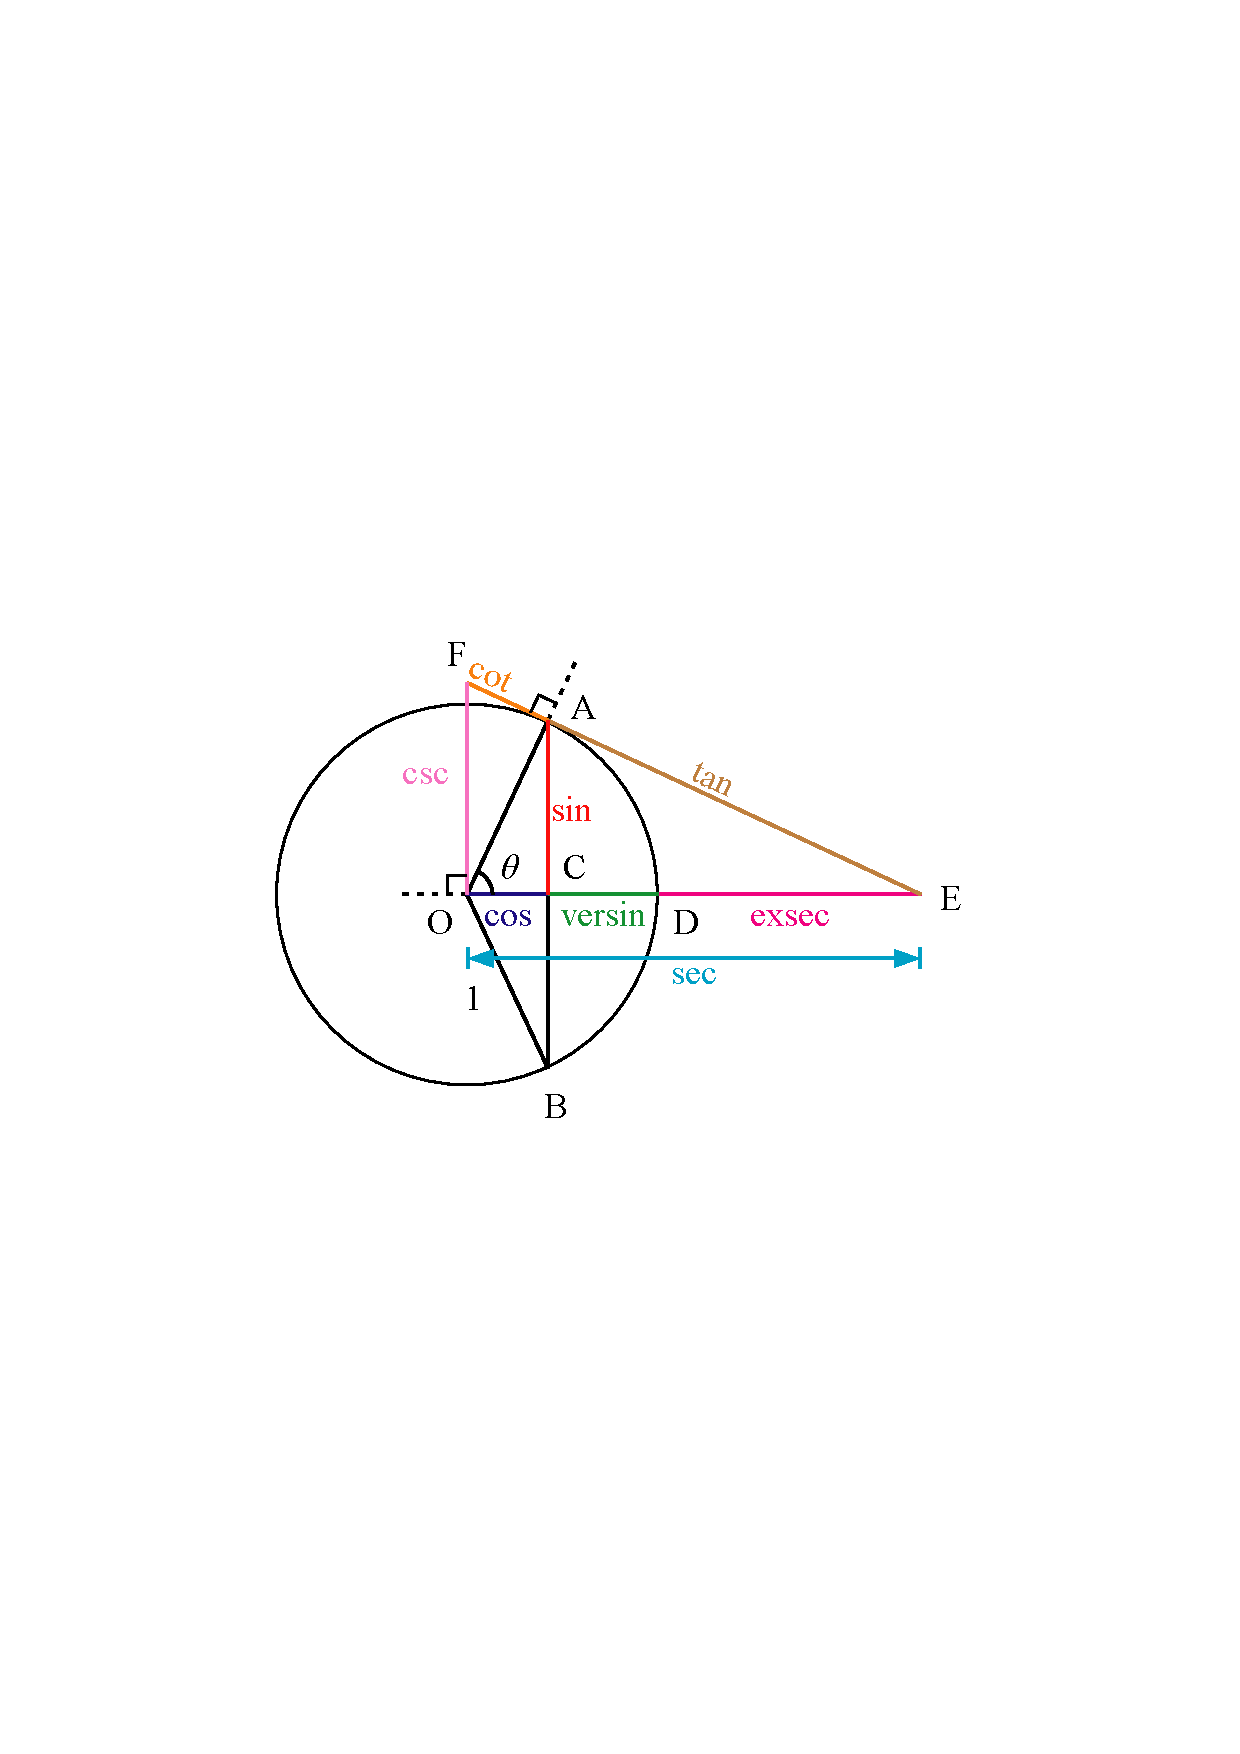
\includegraphics[width=9cm]{einheitskreis.pdf}
			
	
	
			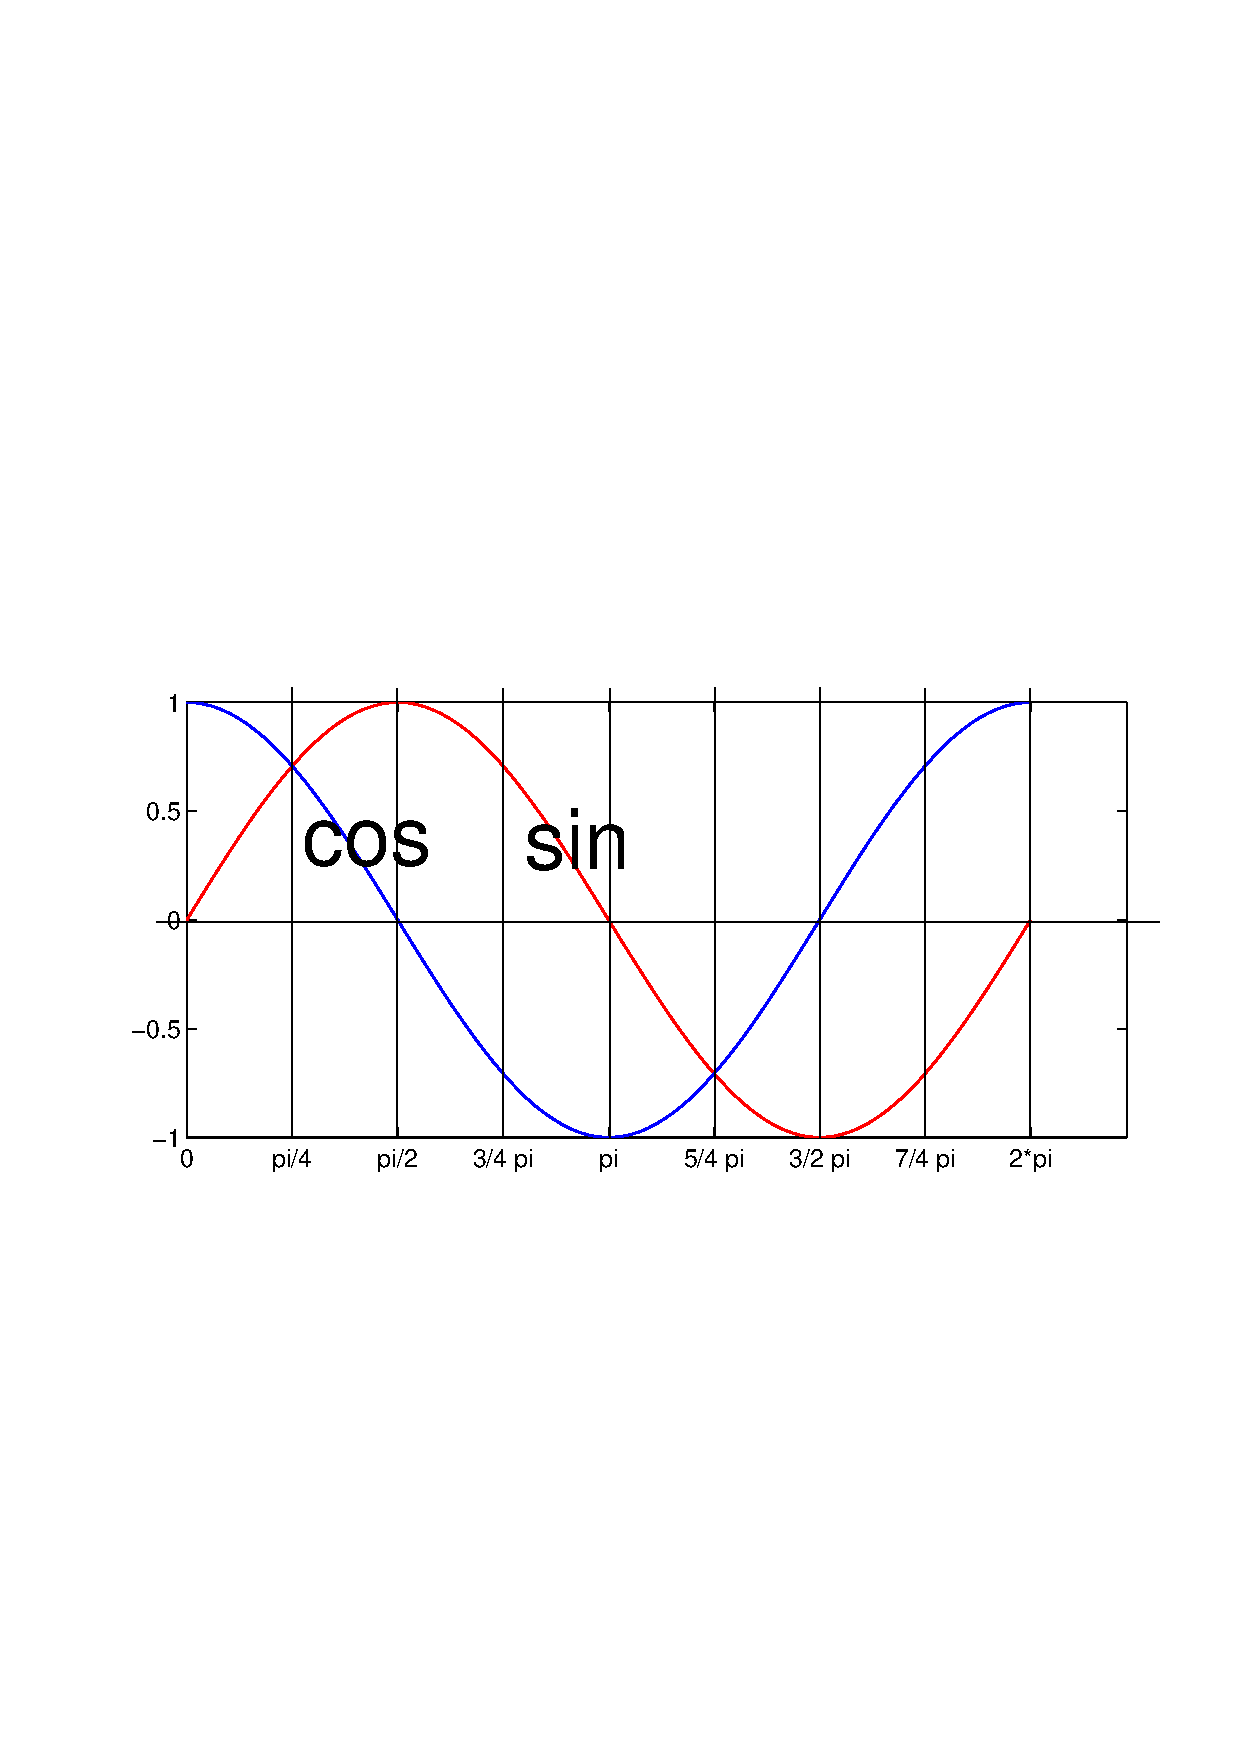
\includegraphics[width=9cm]{sincos.png}
			
			\vspace{4mm}
			\renewcommand{\arraystretch}{1.6}
			\begin{tabular}{r|ccccccc}
			\textbf{Winkel}     &\textbf{0}    &\textbf{30}            &\textbf{45}    &\textbf{60}    &\textbf{90}     &\textbf{180}  &\textbf{270}\\\hline
			\textbf{Bogenmass}  &$0$           &$\frac{\pi}{6}$        &$\frac{\pi}{4}$&$\frac{\pi}{3}$&$\frac{\pi}{2}$&$\pi$          &$\frac{3\pi}{2}$\\\hline
			\textbf{Sinus}      &$0$           &$\frac{1}{2}$          &$\frac{\sqrt{2}}{2}$&$\frac{\sqrt{3}}{2}$&$1$  &$0$            &$-1$\\
			\textbf{Cosinus}    &$1$           &$\frac{\sqrt{3}}{2}$   &$\frac{\sqrt{2}}{2}$&$\frac{1}{2}$&$0$    &$-1$           &$0$\\
			\textbf{Tangens}    &$0$           &$\frac{\sqrt{3}}{3}$   &$1$       &$\sqrt{3}$     &-              &$0$            &-\\
			\end{tabular}
% 			\begin{fmerke}[Bernoullische Ungleichung]
% 				$\forall n \in N: (1+x)^n \geq 1+nx$
% 			\end{fmerke}
% 		
% 			\begin{fsatz}[Young]
% 				$\forall x,y \in R, \epsilon > 0: 2\vert xy \vert \le \epsilon^2x^2+\frac{1}{\epsilon^2}y^2$
% 			\end{fsatz}
		
			\subsection{Hyperbolische Funktionen}
				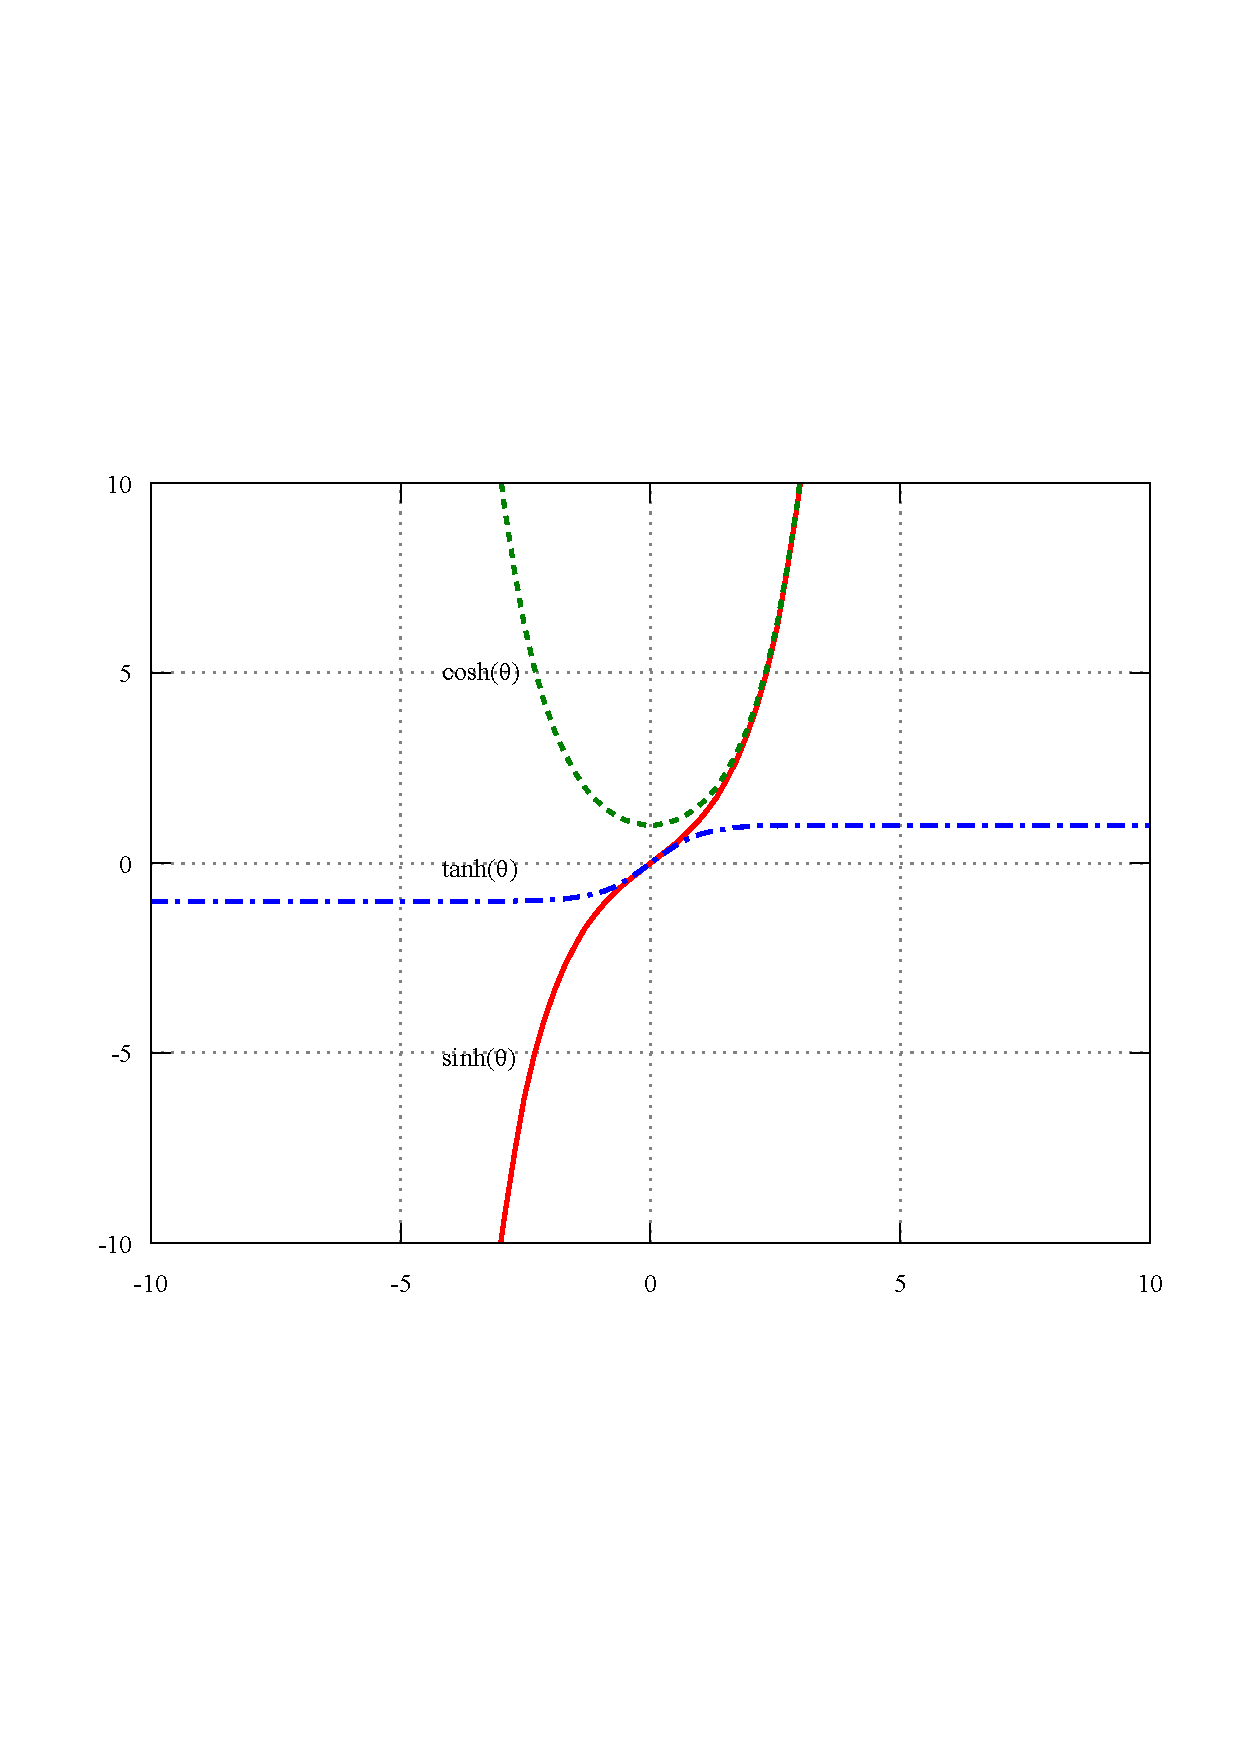
\includegraphics[width=9cm]{Sinh_cosh_tanh.pdf}
			\subsection{Exponentialfunktionen}
				\includegraphics[width=9cm]{ex_ln}
		\end{multicols}

\section{Sonstiges}
	\begin{fmerke}[Partialbruchzerlegung]
		\paragraph{Idee} Gebrochenrationale Funktion zerlegen
		\vspace{-3mm}
		\paragraph{1} Polynomdivision durchführen
			\vspace{-3.5mm}
		\paragraph{2} Nenner des Divisionsrests $q(x)$ faktorisieren, damit Rest umschreiben:
				\vspace{-2mm}
			$$\frac{p(x)}{q(x)} = \frac{A_1}{u_1} + \ldots + \frac{A_n}{u_n} \qquad \text{wobei } u_1 \cdot \ldots \cdot u_n = q(x)$$\\[-3.8mm]
			Beachte: Doppelte Faktoren $u$ müssen bis im Quadrat, Dreifache bis hoch 3 usw. vorkommen! ($\frac{A}{x-1} + \frac{B}{(x-1)^2} + \frac{C}{(x-1)^3} + \ldots$)
			\vspace{-3.5mm}
		\paragraph{3} rechte Seite der oberen Gl. auf selben Nenner bringen
			\vspace{-3.5mm}
		\paragraph{4} $A_1$ bis $A_n$ mit Koeffizientenvergleich und Auflösen eines LGS berechnen
	\end{fmerke}
	
	\begin{fmerke}[Spezielle Taylorreihen]
		\begin{align*}
			e^x &= \sum_{n=0}^\infty		\frac{x^n}{n!}					&&= 1+x + \frac{x^2}{2!} + \frac{x^2}{2!} +  \frac{x^3}{3!} +  \frac{x^4}{4!}\ldots \\
			\sin(x)&= \sum_{n=0}^\infty 	\frac{(-1)^n x^{2n+1}}{(2n+1)!} &&= x - \frac{x^3}{2!} + \frac{x^5}{5!} -  \frac{x^7}{7!} +  \frac{x^9}{9!}-\ldots \\
			\cos(x) &= \sum_{n=0}^\infty	\frac{(-1)^n x^{2n}}{(2n)!}		&&= 1- \frac{x^2}{2!} + \frac{x^4}{4!} -  \frac{x^6}{6!} +  \frac{x^8}{8!}-\ldots\\
			\log(1+x) &= \sum_{n=0}^\infty	(-1)^{n+1}\frac{x^n}{n}		    &&\text{für } -1 \leq x \leq 1
		\end{align*}

	\end{fmerke}

	\begin{fmerke}[Spezialfall Ausklammern]
		\begin{align*}
			(x^n - y^n) = (x-y)(x^{n-1}+x^{n-2}y + \ldots + x y^{n-2}+y^{n-1})
		\end{align*}

		\end{fmerke}
		
	\begin{fdef}[Signum-Funktion]
		\begin{align*}
			sgn{x} = \begin{cases}
							1	& \text{falls }	x > 0 \\
							0	& \text{falls }	x = 0 \\
							-1	& \text{falls }	x < 0\end{cases}
		\end{align*}
	\end{fdef}
	
	\subsection{Flächen, Volumenformeln}
		\begin{tabular}{rl}
			Kreis &$(x-x_0)^2 + (y-y_0)^2 = r^2$\\
			Kugeloberfläche &$(x-x_0)^2 + (y-y_0)^2 + (z-z_0)^2 = r^2$
		\end{tabular}
		
		\subsubsection{Masse von speziellen Gebieten}
			
			\begin{tabular}{rl}
				Zylinder	&$V=\pi r^2 h$\\
				Kegel		&$V= \frac{\pi}{3}r^2 h$\\
				Kegelstumpf	&$V= \frac{\pi h}{3}(r_1^2 + r_2^2 + r_1 r_2)$\\
				Pyramide	&$V= \frac{1}{3}Gh$\\
				Ellipsoid	&$V= \frac{4\pi}{3} abc$
			\end{tabular}	

		
		\subsection{Euklidischer Raum}
		% Kanonische Basis??
			\begin{fmerke}[Euklidische Norm]
				$\Vert x \Vert = \sqrt{\langle x,x \rangle}$
			\end{fmerke}
		
			\begin{feig}[Eigenschaften der Euklidischen Norm]
				\begin{tabular}{l l l}
					positive Definitheit: & $\forall x \in \R^n:$ & $\Vert x \Vert \geq 0, \Vert x \Vert = 0 \Leftrightarrow x=
					0$\\
					positive Homogenität: & $\forall x \in \R^n, \alpha \in
					R:$ & $\Vert \alpha x \Vert = \vert\alpha\vert\Vert x
					\Vert$\\
					Dreiecksgleichung: & $\forall x,y \in \R^n:$ & $\Vert x+y\Vert \leq \Vert x\Vert+\Vert y\Vert$
				\end{tabular}
			\end{feig}
		
			\begin{fmerke}[Cauchy-Schwarz]
				$\forall x,y \in \R^n: \vert \langle x,y\rangle \vert \leq \Vert x\Vert\Vert y\Vert$
			\end{fmerke}
		
			\begin{fregeln}[Euklidische Metrik] $d(x,y) = \Vert x-y\Vert$
			($d$: Distanz)\\
				\begin{tabular}{l l}
					positive Definitheit: & $d(x,y) \geq 0, d(x,y)=0 \Leftrightarrow
					x=y$\\
					Symmetrie: & $d(x,y)=d(y,x)$\\
					Dreiecksgleichung: & $d(x,z) \leq d(x,y) + d(y,z)$
				\end{tabular}
			\end{fregeln}
				
			\begin{fmerke}[Metrik]
				Eine Abbildung $d: M \times M \rightarrow \R$ heisst Metrik
				auf $M$, falls gilt:\\
				$d(x,y) \geq 0, d(x,y) = 0 \Rightarrow x=y$\\
				$d(x,y) = d(y,x)$\\
				$d(x,z) \leq d(x,y)+d(y,z)$
			\end{fmerke}
			
		\subsection{Konstanten}			
			\begin{fmerke}[Eulersche Zahl]
				$a_n = (1 + \frac{1}{n})^n < b_n= (1 + \frac{1}{n})^{n+1} \quad n\in \N$
			\end{fmerke}
		
			\begin{fmerke}[Goldener Schnitt]
				$g = 1 + \frac{1}{g}$ \quad $h = \frac{1}{g}:=$ Goldener
				Schnitt
			\end{fmerke}
	\end{appendix}
	
\end{document}
